\documentclass[zihao=-4,fontset=none]{Beautybook-CN}
\coverstyle={ % 封面键值列表
    cover-choose=cn, % cn (需新增项\entitle{#}); en ; enfig ; birkar
}
\mathstyle={ % 数学字体键值列表
    math-font=plain, %plain (默认数学字体); mtpro2
}
\RequirePackage{stys/settings-CN}
\usepackage{zhlipsum}
\begin{document}
\thispagestyle{empty}
\entitle{Live in XJTU Medical School} % cncover专用
\title{西安交通大学医学部生活指南}
\subtitle{复代数几何学笔记}
\edition{First Edition}
\bookseries{From students, for students}
\author{本书编委会}
\pressname{正在编辑中出版社}
\presslogo{inner_pics/Springer-logo.png}
\coverimage{inner_pics/coverimage.jpg} % cncover专用
%\coverimage{inner_pics/ivy-ge998908f8_1280.jpg}
\makecover % 封面生成命令

% 主题色调
\definecolor{bg}{HTML}{e0e0e0}
\definecolor{fg}{HTML}{203A43}
\colorlet{outermarginbgcolor}{bg}
\colorlet{outermarginfgcolor}{fg}
\colorlet{framegolden}{fg}
\colorlet{framegray}{黛绿!5}
\colorlet{headlinecolor}{靛蓝}
\chapoddimage{inner_pics/songodd.png}
\chapevenimage{inner_pics/songeven.png}
% set the contents of the outer margin on even and odd pages for scrheadings, plain and scth
\oddoutermargin{\cabin\leftmark} % Odd 奇数页
\makeatletter
\evenoutermargin{\cabin\@title} % Even 偶数页
\setlength\footheight{25pt}
\ofoot{} % 页脚信息
\makeatother
%
\thispagestyle{empty}
\begin{titlepage}
\thispagestyle{empty}
    \begin{center}
    
    %% Print the bookseries
    {\makeatletter
    \ifdefvoid{\@bookseries}{}{\bigskip\normalfont\fontsize{20}{20}\selectfont\@bookseries}
    \makeatother}

        \bigskip
        \bigskip

    %% Print the title
    {\makeatletter
    \fontsize{35}{35}\rmfamily\bfseries\selectfont\@title
    \makeatother}
    
    \bigskip
    \bigskip
    
    \bigskip
    \bigskip
    \bigskip

    %% Print the name of the author
    {\makeatletter
\vspace{8em}
    \fontsize{25}{25}\rmfamily\bfseries\selectfont 本书编委会(排名不分前后)
    \bigskip

    \begin{table}[h]
    \centering
    \fontsize{20}{20}\rmfamily\mdseries\selectfont
\begin{tabular}{llll}
lyc  & gzh   & lky  & xkr   \\
小鱼   & 徐小黑   & 小旋风  & 玉子烧战士 \\
小小旋风 & 西曦小朋友 & 选手小车 & 某人    \\
拉莫三嗪 & 小尾巴   & 唐抒欢  & 垃圾桶  
\end{tabular}
\end{table}
    % \fontsize{25}{25}\rmfamily\mdseries\selectfont{lyc \hspace{1em} gzh \hspace{1em} \hspace{1em} lky \hspace{1em} xkr \\ 小鱼 \hspace{1em} 徐小黑 \hspace{1em} 小旋风 \hspace{1em} 玉子烧战士 \\ 小小旋风\hspace{1em} 西曦小朋友 \hspace{1em}选手小车 \hspace{1em}某人 \\ 拉莫三嗪\hspace{1em} 小尾巴\hspace{1em} 唐抒欢\hspace{1em} 垃圾桶}
    \makeatother}
    
    \bigskip
    \bigskip

    
    \vfill
    
    
    \bigskip
    \bigskip
    
    {\makeatletter
    \fontsize{25}{25}\rmfamily\selectfont\@pressname
    \makeatother}
    \end{center}
    
    \end{titlepage}
    \let\cleardoublepage\clearpage

    \thispagestyle{empty}
    \begin{center}
        {\fontsize{20}{20}\rmfamily\selectfont    内\hspace{1em}容\hspace{1em}简\hspace{1em}介}\\ 
        \bigskip

        本书是由西安交通大学医学部的二十余位本科生编写的生活指南,内容涵盖学习、科研、升学、娱乐、校园活动等多个方面,是医学部创建以来第一部由学生自发组织、编纂的综合性指南。本书紧紧围绕“From students, for students”的初心,对稿件质量层层把关,致力打造权威科学、质量过硬的高标准指南,对本校医学部的人才培养和学生发展起到不可多得的指导作用。
        \bigskip
        
        This book is a guide to life written by more than 20 undergraduate students from the Medical School of Xi'an Jiaotong University. The content covers various aspects such as learning, scientific research, further education, entertainment, and campus activities. It is the first comprehensive guide organized and written by students since the establishment of the Medical School. This book closely adheres to the original intention of "From students, for students" and strictly controls the quality of manuscripts in order to create an authoritative and high-quality standard guide. It plays an invaluable guiding role in the development of students in our medical school.

        \bigskip

        {\fontsize{10}{10}\rmfamily\bfseries\selectfont 图书在版编目(CIP)数据}\\[-2ex]
        \tikz\draw[line width=1pt,black] (0,0)-- (.99\linewidth,0);\\[-.8ex]
        西安交通大学医学部生活指南/(中)本书编委会著 --西安; 正在编辑中出版社,2023.09 \\ 
        {\bfseries ISBN: } 978-7-03-002970-6\\ 
        I.西……\circled{1} 本……\\ 
        中国版本图书馆CIP数据核字(2023)第00022893号\\[-2ex]
        \tikz\draw[line width=1pt,black] (0,0)-- (.99\linewidth,0);\\[-.8ex]
        {\itshape 责任编辑: Zhonghao / 责任校对: Zhonghao\\ 
        责任印刷: Zhonghao}
        \vfill

        {\makeatletter
    \fontsize{10}{10}\rmfamily\selectfont\@pressname 
    \makeatother}出版\\ 
    {\footnotesize 陕西省西安市雁塔区小寨路街道雁塔西路76号西安交通大学医学院}\\ 
    \href{https://lycsplanet.com/}{lycsplanet}\\ 
    {\fontsize{10}{10}\rmfamily\selectfont 陕西省印刷有限公司} 印刷\\ 
    正在编辑中出版社发行\hspace{2em} 各地新华书店经销\\ 
    \bigskip
    *\\
    \bigskip
    {\footnotesize\begin{tabular}{ll} 2023年09月第一版 & 开本: $850\times1168\quad \quad1/32$\\ 
    2023年09月第一次印刷 & 印张: $18 5/8$\\ 
    \multicolumn{2}{c}{字数:46 742}\\
    \end{tabular}}\\ 
    {\fontsize{10}{10}\rmfamily\bfseries\selectfont 定价: 89.00元}\\ 
    {\footnotesize (如有印刷问题,我社负责调换)}


    \end{center}





 % 内封面页
%
\frontmatter % 前置材料
\pagenumbering{Roman}
\thispagestyle{empty}
\addcontentsline{toc}{chapter}{前言}
\chapter*{前言}
想写这个指南其实是大二还是大三暑假看见上交版本,觉得很好却再也没有其他学校,心想如果能有更多的指南该多好,要不快毕业时写一下吧,于是此时此刻我拉了很多善良的朋友们一起完成这个医学部指南,希望它能对大家有用,希望能有更多的人参与编辑工作,让它持续更新下去。我会将文档无偿分享,并放在github与我的个人网站上。

如何度过医学部大学生活呢,每个人都有不同的经历,其中有无数道关卡等待着大家,希望本篇指南能对大家起到抛砖引玉的作用\textasciitilde{}

此篇指南未经作者授权,任何组织或个人都不得违反版权法规,包括但不限于抄袭、转载、摘编或修改此指南的内容。本指南的使用限于非商业目的,未经许可不得扭曲、修改或广泛传播。本指南提供了观点和见解,但不构成具体的行动建议,作者对因使用本指南而产生的后果不承担责任。本指南的作者无法保证其内容不会导致对其他组织的误解或偏见,而且未经专业审查,因此其准确性不能得到保证。请大家根据个人情况自行分辨。



\hfill 
\begin{tabular}{lr}
    &----- lyc\\ 
&2023年 09月 13日
\end{tabular}

\let\cleardoublepage\clearpage % 前言
\thispagestyle{empty}
\tableofcontents\let\cleardoublepage\clearpage % 目录

\mainmatter % 正文
\pagenumbering{arabic}
\partimage{inner_pics/part.png}
\partabstract{\hspace{2em}本部分从多个角度提出医学生如何在课程学习、科学研究、升学出国等方面快人一步。专业课学习部分侧重于如何提高绩点,同时介绍了一些不错的学习资源。英语学习分为应试部分和应用部分。科研部分综合了多位优秀科研大佬的经验。升学与出国深造部分介绍了多种本科完成后继续接受教育的路径。除此之外,我们还邀请两位医学部优秀人才撰写了两篇特别内容,分别介绍如何润出医学部而转去其他专业,以及如何在基础医学科研领域拔得头筹。
		
	\hspace*{2em} \sffamily{This chapter provides insights on how medical students can gain an advantage in various aspects such as course learning, scientific research, and further study abroad. The section on course learning focuses on improving GPA and introduces valuable learning resources. The English section is divided into exam preparation and practical application. The scientific research section incorporates the experiences of accomplished researchers. The chapter on further study and studying abroad introduces multiple options for continuing education after completing the undergraduate program. Additionally, two exceptional talents from the medical department have been invited to contribute special content to this book, outlining strategies for smoothly transitioning to a different field from the medical department and excelling in basic medical research. }}
\part{学习部分}

\chapter{专业课学习(GPA)}
\section{合适的学习路径}

对于大学课程的学习,我们基本可以分为三种学习路径:
\begin{enumerate}
	\item 平时\textbf{认真}听课,课后\textbf{积极}预习、复习,考前认真准备
	\item 平时\textbf{完整}听课,课后\textbf{没有}预习、复习,考前认真准备
	\item 平时\textbf{不}听课,课后\textbf{没有}预习、复习,考前\textbf{突击}准备
\end{enumerate}

经过五年的课程和考试的磨练,我们认为\textbf{第2种}学习路径是最为可取的。原因如下:
\begin{enumerate}
	\item 平时认真的学习,对考试的帮助难以定量。
	      \begin{itemize}
	      	\item 考试内容有相当比重的一部分来自于往年题和老师画的重点,考前认真准备完全可以覆盖。
	      	\item 很难坚持一个学期都认真学习,而一旦中间有一两节课落下了,后面就完全跟不上。
	      \end{itemize}
	      	      
	\item 平时认真的学习,不一定能帮助到未来的课程。因为这门课考过之后就很难有机会再捡起来,难以在脑中留下长时间的记忆。
	\item 平时如果不听课,就不能记录到老师随口画的重点,这对于考试是一个不小的劣势。
	\item 将课余时间用于更多富有意义的事,您将收获更加多姿多彩的大学时光。
\end{enumerate}
\section{必备的学习资源}

以下按照重要性,由大到小进行排序。

\subsection{往年考试题(必看!)}

\begin{itemize}
	\item 资源位置:
	      \begin{enumerate}
	      	\item 微信公众号\textbf{“学濂”}中“精选习题”栏目,见\ref{fig:xuelian}:
	      	      	      	      
	      	      \begin{figure}[htbp]
	      	      	\centering
	      	      	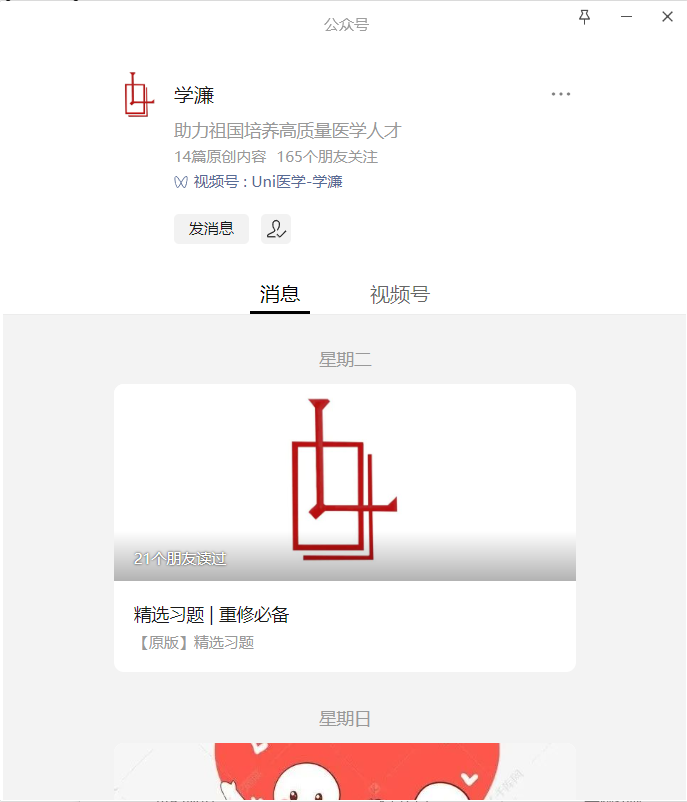
\includegraphics[width=1\textwidth]{media/image1.png}
	      	      	\caption{微信公众号\textbf{“学濂”}}
	      	      	\label{fig:xuelian}
	      	      \end{figure}
	      	      	      	      
	      	      优点:汇总了各种途径的往年题,并且有学濂自己编写的参考答案。
	      	      	      	      
	      	      缺点:参考答案有时出现错误。
	      	\item QQ群\textbf{“XJTU-MEDer”}中“密谈系列”
	      	\item 微信公众号\textbf{“ A HORCRUX”}中往年题
	      \end{enumerate}
	      	      
	\item 使用方法:考试前需熟练掌握往年题中涉及的知识点,最好能把简答题和论述题的答案记下来。
\end{itemize}
\subsection{学习资料}

\paragraph{\textbf{老师的PPT\textnormal{(推荐程度${\bigstar}$${\bigstar}$${\bigstar}$${\bigstar}$${\bigstar}$)}}}


\begin{itemize}
	\item 资源位置:班级群
	      	      
	      优点:一手内容,考试题的来源,可信度最高。
	      	      
	      缺点:内容太多,无法遍历;重点不突出,看完感觉和没看一样。
	\item 使用方法:一轮复习时可以过一遍,不求完全掌握,有个印象就好。
\end{itemize}
\paragraph{\textbf{“学濂”课堂笔记\textnormal{(推荐程度${\bigstar}$${\bigstar}$${\bigstar}$${\bigstar}$${\bigstar}$)}}}


\begin{itemize}
	\item 资源位置:微信公众号“学濂”中“课堂笔记”栏目
	      	      
	      优点:多数为同年级同学根据老师上课讲的重点整理,实用性高。
	      	      
	      缺点:经常在考试前一两天才发出来,没时间看。
	\item 使用方法:看完往年题后,有时间可以过一下。
\end{itemize}
\paragraph{\textbf{思维导图\textnormal{(推荐程度${\bigstar}$${\bigstar}$${\bigstar}$☆☆)}}}


\begin{itemize}
	\item 资源位置:哔哩哔哩up主“卡尔拉的洛克白”
	      	      
	      \url{https://space.bilibili.com/34127448/}
	      	      
	      优点:简明易懂,层次清楚。
	      	      
	      缺点:很多大纲内容没有涉及。
	\item 使用方法:在对课程毫无概念的情况下,这是一部不错的入门教程,可以帮你快速把握课程的大概内容。
\end{itemize}
\paragraph{\textbf{各种题库}}


\begin{itemize}
	\item \textbf{医考帮}(推荐程度${\bigstar}$${\bigstar}$${\bigstar}$${\bigstar}$${\bigstar}$)
	      \begin{itemize}
	      	\item 优点:考研题,难度较高,准确度高,学到的知识多;解析详细,评论区有许多奇妙的口诀,帮助记忆。
	      	\item 缺点:部分内容与本校大纲不符,需酌情选择试题;很多科目考研不考,需切换题库为执业医师考试或本科考试(个人推荐执业医师考试,因为评论区较活跃);今年起出现限制题库使用的情况,部分同学转战“蓝基因”app.
	      \end{itemize}
	      	      
	\item 人民卫生出版社的\textbf{《${\times}$${\times}$科学习指导与习题集》}(推荐程度${\bigstar}$${\bigstar}$${\bigstar}$${\bigstar}$☆)
	      \begin{itemize}
	      	\item 优点:难度适中,覆盖面广;有简答题及论述题。
	      	\item 缺点:数量太多,做不完;有错题;部分内容与本校大纲不符,需酌情选择试题。
	      \end{itemize}
	      	      
	\item 使用方法:在明确每一章大纲的情况下,做医考帮上的选择题,过一遍学习指导上的简答题及论述题。
\end{itemize}
\subsection{日常学习的教材推荐}

在学习的过程中,本人发现许多优秀的教材,可以起到辅助甚至替代人卫教材的作用,帮助您在日常学习中如虎添翼,一骑绝尘。

\paragraph{\textbf{全科目}}


\begin{itemize}
	\item \textbf{人卫五年制第九版教材}(推荐程度${\bigstar}$${\bigstar}$${\bigstar}$${\bigstar}$☆)
	      \begin{itemize}
	      	\item 优点:最权威,万法之宗。
	      	\item 缺点:太厚,看不完;缺乏记忆方法。
	      \end{itemize}
	      	      
	\item \textbf{人卫八年制第三版教材}(推荐程度${\bigstar}$${\bigstar}$${\bigstar}$${\bigstar}$☆)
	      \begin{itemize}
	      	\item 优点:有些地方比五年制教材解释得清楚,据说五年制教材是照着八年制抄的。
	      	\item 缺点:缺乏一些新的指南(如诊断标准)。
	      \end{itemize}
	      	      
	\item 建议:以五年制教材为主,有看不懂的地方就翻翻八年制教材,看看有没有详细的解释。
\end{itemize}
\paragraph{\textbf{生物化学、生理学、病理学、内科学、外科学(考研科目)}}


\begin{itemize}
	\item \textbf{贺银成考研讲义}(推荐程度${\bigstar}$${\bigstar}$${\bigstar}$${\bigstar}$${\bigstar}$)
	      \begin{itemize}
	      	\item 优点:家喻户晓、有口皆碑,是您案头不可缺少的好伙伴!众多精妙的表格和记忆方法,源于教材而超出教材。
	      	\item 缺点:与学校大纲有些许出入。
	      \end{itemize}
	      	      
	\item 傲视天鹰、医考帮等其他考研讲义,本人没有深入使用过,您可以自己尝试。
\end{itemize}
\paragraph{\textbf{药理学、医学微生物学、医学免疫学、解剖学、病理生理学、医学心理学、医学伦理学、妇产科学、儿科学、精神神经系统(执业医师考试科目)}}


\begin{itemize}
	\item \textbf{贺银成执业医师考试讲义}(推荐程度${\bigstar}$${\bigstar}$${\bigstar}$☆☆)
	      \begin{itemize}
	      	\item 优点:贺银成出的,把重点内容提炼出来了。
	      	\item 缺点:质量远远逊于考研讲义,基本是照抄课本。
	      \end{itemize}
	      	      
\end{itemize}
\paragraph{\textbf{药理学}}


\begin{itemize}
	\item \textbf{《图表药理学》}袁秉祥 / 臧伟进;人民卫生出版社(推荐程度${\bigstar}$${\bigstar}$${\bigstar}$${\bigstar}$${\bigstar}$)
	      \begin{itemize}
	      	\item 优点:以图表方式讲述药理,格式清晰易懂,内容深入浅出。本人在药理学课程完结后仍时常翻阅,深感其常看常新!
	      	\item 缺点:无。
	      \end{itemize}
	      	      
\end{itemize}
\paragraph{\textbf{病理生理学}}


\begin{itemize}
	\item \textbf{《病理生理学(第二版)》}黄宁 / 赵敬;科学出版社(推荐程度${\bigstar}$${\bigstar}$${\bigstar}$${\bigstar}$${\bigstar}$)
	      \begin{itemize}
	      	\item 优点:内容深刻,解释全面,逻辑通顺,私以为编者水平超过人卫版本。
	      	\item 缺点:有些内容在理解上有难度。
	      \end{itemize}
	      	      
\end{itemize}
\paragraph{\textbf{心电图(诊断学、内科学中重要章节)}}


\begin{itemize}
	\item \textbf{《明明白白心电图(第四版)》}柳俊 / 王莺;广东科技出版社(推荐程度${\bigstar}$${\bigstar}$${\bigstar}$${\bigstar}$${\bigstar}$)
	      \begin{itemize}
	      	\item 优点:以漫画形式帮您领会艰深晦涩的心电图知识,教会您如何快速判断心电图;少有的可以比肩国外教材水平的书。
	      	\item 缺点:无。
	      \end{itemize}
	      	      
\end{itemize}
\paragraph{\textbf{中医学}}


\begin{itemize}
	\item \textbf{《中医考研学霸笔记》}(推荐程度${\bigstar}$${\bigstar}$${\bigstar}$${\bigstar}$☆)
	      \begin{itemize}
	      	\item 优点:各种表格和总结,方便背诵。
	      	\item 缺点:内容远远超过大纲范围。
	      \end{itemize}
	      	      
\end{itemize}
\subsection{网课推荐}

\begin{example}
	宗旨:考研科目和执医科目以专门考试机构的网课为佳(如贺银成、昭昭、医考帮等),除此之外有几门较为推荐的网课我会写在下面。
\end{example}

\paragraph{\textbf{系统解剖学}}


\begin{itemize}
	\item 霍琨老师-人体解剖学-系统解剖学全集【59级全集·更新完结】(推荐程度${\bigstar}$${\bigstar}$${\bigstar}$${\bigstar}$${\bigstar}$)
	      	      
	      \url{https://www.bilibili.com/video/BV1jf4y1C7LM/}
	      \begin{itemize}
	      	\item 优点:手绘板书,深入浅出,讲解清楚,前无古人、后无来者。唯一一门建议不听学校老师的课,听这个吧!
	      	\item 缺点:无。
	      \end{itemize}
	      	      
\end{itemize}
\paragraph{\textbf{考研/执医机构网课比较}}\mbox{}\\
平心而论,各个做考研辅导的机构都有一定的底子,网课质量没有明显的优劣之分,更多是风格的不同,您可以选择适合自己的网课学习。
\begin{itemize}
	\item 贺银成(推荐程度${\bigstar}$${\bigstar}$${\bigstar}$${\bigstar}$${\bigstar}$)
	      \begin{itemize}
	      	\item 优点:非常经典;口音奇特,听多了会魔音入脑;有很多口诀。
	      	\item 缺点:无。
	      \end{itemize}
	      	      
	\item 刘忠保(推荐程度${\bigstar}$${\bigstar}$${\bigstar}$${\bigstar}$${\bigstar}$)
	      \begin{itemize}
	      	\item 优点:真正的大师,风华绝代,如果说我大学有崇拜过什么老师的话,就是保哥了;能帮您把很多知识点都穿起来;不仅教书,还教给您为人处世的道理;推荐生理学和内科。
	      	\item 缺点:视频太长,有一些“废话”;不建议用于考前复习,适合日常听。
	      \end{itemize}
	      	      
	\item 昭昭(推荐程度${\bigstar}$${\bigstar}$${\bigstar}$${\bigstar}$${\bigstar}$)
	      \begin{itemize}
	      	\item 优点:在白板上写字、画图,图文结合,方便理解;适合于零基础学习,深度可能不够。
	      	\item 缺点:节奏有点慢。
	      \end{itemize}
	      	      
	\item 医考帮(推荐程度${\bigstar}$${\bigstar}$${\bigstar}$${\bigstar}$${\bigstar}$)
	      \begin{itemize}
	      	\item 优点:内容重点突出,讲课有激情;推荐唐子益(内科)、徐琦(外科)。
	      	\item 缺点:无。
	      \end{itemize}
	      	      
	\item 医学教育网(推荐程度${\bigstar}$${\bigstar}$${\bigstar}$${\bigstar}$${\bigstar}$)
	      \begin{itemize}
	      	\item 优点:偏向执医课程,考研科目之外的可以看看,口诀很有用;推荐景晴(病理生理学)、汤以恒(药理学)。
	      	\item 缺点:不够深入。
	      	      \begin{example}
	      	      	汤以恒的\href{https://docs.qq.com/doc/DZXRuZXVGZktRSFhM}{药理学口诀}。
	      	      \end{example}
	      \end{itemize}
	      	      
	\item 刘不言(推荐程度${\bigstar}$${\bigstar}$${\bigstar}$${\bigstar}$${\bigstar}$)
	      \begin{itemize}
	      	\item 优点:推荐生物化学课,我本人没听过,但听过的都说好。
	      	\item 缺点:无。
	      \end{itemize}
\end{itemize}
\chapter{英语}
以下按照是否以提升考试成绩为目标,分为应试部分和应用部分。
\section{应用部分:}
\subsection{态度}
\begin{itemize}
\item \textbf{兴趣是最好的老师},语言学习不在于学习这门语言本身,而是利用它找到自身感兴趣的话题然后在感兴趣的话题中学习利用它,自然会产生对语言的兴趣,从而才能坚持学习。
\item \textbf{坚持一定会有收获},每个人都至少会一门语言,那说明每个人都有语言的天赋,一定是可以学好语言的,一定要给自己信心不断坚持。
\end{itemize}
\subsection{听}
\begin{itemize}
\item 各类podcast(如NPR或其他个人播客) 建议有一定英语基础后再听。
\item 浏览大量英文视频 如Youtube或无中文字幕英美剧。
\item 先听VOA慢速英语,可以完全听懂再转换到常速新闻,能听懂标准的说法再去接触网上有俚语/网络用语的视频或音频。
\end{itemize}
\subsection{说}
\subsubsection{真人练习}
\begin{itemize}
\item \href{https://www.cambly.com/english?lang=zh_CN}{Cambly}平台:使用体验不错,建议打折时购入,先免费体验20分再决定花钱与否 。
\item Hellotalk、Meetup等平台
\end{itemize}
\subsubsection{AI练习:}
\begin{itemize}
\item 利用Chatgpt:下载Vioce control for chatgpt  这个Chrome插件。
\item Call Annie 需要IOS美区账号才能下载APP, 其实也有web端可以不用美区账号。
\end{itemize}
\begin{example}
    建议可以两种都尝试一下,真人可以随时给你提出错误,改正完善,以及和真实的不同国家的人对话也可以感受一下,AI反应也很迅速,没有任何交流障碍,最重要的是免费真的很香。
\end{example}
\subsection{读}
\begin{itemize}
\item 外刊

虽然非常多人推荐,但个人体验是没有产生兴趣,完全无法坚持阅读 (补充:建议先试试看!没必要篇篇都读,可以挑选自己原本就感兴趣的领域。很多人推荐也是个人用过觉得很好的三本:基督教科学箴言、The Atlantic、The Economist,难度升序排列)。
\item 订阅感兴趣的newsletter阅读 \url{https://feedx.net/} 或者\url{https://substack.com/}两个网站都可以订阅 或者各种博主自己的newsletter.
\item 各种类型的英文电子书  \url{https://annas-archive.org/} 可以在此网站找到大多数电子书。
\item 各种英文社交平台如 Reddit ,Twitter等等。
\end{itemize}
\subsection{写:}
\begin{itemize}
\item 找寻语言交换伙伴,我在reddit找到的,各种语言交流社群都会有。
\item \href{https://slowly.app/}{Slowly} 找寻不同国家笔友。
\item 练习雅思托福作文,利用AI评分改进。
\end{itemize}
\section{应试部分}
\subsection{托福攻略}

\subsubsection{写在前面}
托福虽然是应试考试,但是打铁还需自身硬,英语能力必然是托福高分的必须,不过我们也可以通过学习托福来提高自己的英语能力啦$\thicksim$

\subsubsection{资源}
\begin{itemize}
\item 托福往年题必备(虽然托福改革了,但是听力阅读依旧有借鉴意义)。
\item b站up主:野性猛哈哈520 (托福阅读真题,推荐练习,运气好考试遇原题)。
\item 口语:改革了,没得独立口语了,好好练tpo叭。
\item \href{https://pan.baidu.com/s/10RPth1ll1xcbwxcw_V7Oaw}{托福四科真题}(提取码:jb2e)

\begin{theorem}
    这部分真题中写作参考性较低(因为改革了)。
\end{theorem}
\item 听力:很难搞到原题,以上链接中有一部分,可以作为考前模拟,感受一下托福听力真题的难度,但小站托福没有的tpo可在知乎 英语喵English 处找到
\end{itemize}

\subsubsection{碎碎念}
\begin{enumerate}
\item 托福考试对考生的听力要求很高,从听力这一个part就可以体现,听力内容为学科讲座,其中生物类主题最为简单(可能和咱们专业与生物医学相关有关),所以实战中很难遇到生物类考题(ETS你真的{\fontspec{Symbola}\char"1F605}),下一个level是天文类和地质类,最难的是人文艺术类,现在的组合模式基本都是天文地质加人文艺术。听力篇幅较长,一篇基本在5分钟左右,语速快,且听完所有内容后才能开始答题,考试对学生的要求就是能听懂,纯靠蒙基本很难答对。可去学习听力记笔记法,不过经实战我觉得有利有弊,能听懂的文章记的笔记可以起到提示作用,听不懂的部分记得笔记还是没一点用,还会占用专注度,不如认真听拿的分数高,还是建议大家在时间允许的情况下认真练托福听力,考完后听力水平会有质的飞跃,阅读和听力在考完这两个part就可出分,建议听力基础薄弱又急于出分的同学转战雅思。
\item 如果你的目标分较低,比如90分,不要过于担心,托福很容易在短时间达到该目标分,托福的卷都发生在高分段{\fontspec{Symbola}\char"1F602}

\item 考试时间不要拖太长,冲刺大概一个月就够用。
\begin{enumerate}
\item 背单词(不用多说,背单词没有捷径,背个大概70\%就可以去考),背完单词基本阅读就没啥问题,很简单。
\item 听力:用tpo,可以听写原文,不过太浪费时间,听写你没听懂的部分就可以,注意语调和连读的适应
\item 口语:每天一篇tpo,练改革后的部分,跟读英语广播或者其他听力资料练习美式语音语调。语音语调还是蛮重要的。
\item 速成背模板法,写作要有逻辑,按照英文写作结构来写,切忌英文拼写错误和语法错误,多选择替代词,不要一个单词用到底,体现你的英文功底,篇幅不能短,但也并不是写的越多分越高(亲测{\fontspec{Symbola}\char"1F62D}{\fontspec{Symbola}\char"1F62D}{\fontspec{Symbola}\char"1F62D}),但会给点辛苦分叭。建议一天一篇练习。
\end{enumerate}
\end{enumerate}
\subsection{雅思攻略}

\subsubsection{写在前面}
\begin{enumerate}
\item 与托福(纯粹学术导向)不同,雅思考试涵盖的生活应用场景明显更多(A类的写作和后几篇阅读还是很学术的,但听力除了最后一篇以及口语就是纯纯生活应用了)。这直接导致了以下两点:雅思会相对更好考到目标分数,以及雅思考试的不确定性更高。
\item 我自己其实是几乎裸考(只在考前做了两套题)的雅思到8.5,但有志愿地帮助学妹准备雅思考试并达到目标分数,下面的内容虽然我没有亲身实践过,但算是验证过。(p.s. 如果你六级能考到600+,雅思裸考7分是可行的,可以跳过下面的内容了)
\end{enumerate}
\subsubsection{资源}
\begin{enumerate}
\item 剑雅官方真题(4-18):雅思的一个好处在于,真题是非常容易获取的。真题带音频,听力和阅读用这套书就可以了,足够用了。答案里会附着写作范文,但一般是7分左右的文章,从模仿价值来看不如下面会讲到的顾家北老师书中的文章,但可以作为“我要写成什么样才能拿到7分”这种问题的最佳参考。建议先做最新的17,18,然后从10开始向后做起,如果还有时间和精力再做10之前的(倒序)。
\item 顾家北:分为写作书和词伙书(这个可能是顾老师创造的概念,简单来讲就是通过含义、词根、应用场景等各个角度寻找单词、词组之间的联系)。写作书非常有用,(真的是手把手教你)即使完全没有英文学术写作的基础,也可以通过这本书学会如何写出像样的雅思作文。词伙书个人认为对于追求7分左右的同学有些趣味性大于实用性了,但如果你想追求更高分,可以参考里面的同义替换等等。
\item 雅思哥app:主要用来练口语。有着很全的口语考题和(由无数烤鸭贡献的)本考季考题出现频率。非常推荐。
\item 官网:资源有限,但上面的 IELTS Progress Check (官方免费模拟考)很有用。毕竟一次两千多块钱,还是确保准备充分再上考场啦!
\end{enumerate}
\subsubsection{Miscellany}
\begin{enumerate}
\item 虽然我前面说了雅思和托福的区别,但共同之处还是有不少的。看到这里的同学们可以把上面关于托福的内容对照着看看。
\item 现在很多英联邦国家的学校也承认托福成绩,相应地,北美也有很多学校承认雅思成绩(比如我就是用雅思成绩申到的JHU夏校和现在在Notre Dame的RA职位)。大家实际上可以根据自身的特点选择考哪一个(比如有的人和机器对话会比和人对话更自在,为了避免社恐影响口语发挥,建议考托福)。
\end{enumerate}
\subsection{四六级攻略(待补充)}
\chapter{科研}
\begin{example}
    如何找导师、如何在寒暑假期间参加科研交流、如何探索基础医学科研领域,请查看\hyperref[sp2]{特别篇(2):基础医学的科研与深造}与\hyperref[basexp]{特别篇(4):XJTU基础医学生存指南 > 关于科研训练}。
\end{example}
\begin{enumerate}
    \item 最重要的

    主动才会有故事,如果你想做任何事情,\textbf{请主动争取},科研同样,甚至你可以在大一初始就开始接触(写到这本人就开始后悔我怎么这么躺)。
    \item 如何寻找

    你可以直接主动在课下询问老师是否可以加入课题组学习,或者在学校网站搜寻心仪导师直接邮件询问
\end{enumerate}

\begin{example}[title=小雷的建议]

    \begin{enumerate}
\item 越早进实验室越好。
\item 多学多看多听,不要狂妄自大,而是要问自己是否真的能够独立自主进行每一个过程。
\item 多读paper,尤其是cns中的super one.
\item 多和pi聊天,吸取他们的科研方法。
\item 多看大佬,看大佬如何发paper,如何定义自己的问题。
\end{enumerate}
\end{example}
\chapter{升学}
\section{考研(待补充)}
\section{保研}
\begin{example}
    更多内容,可查看\hyperref[basebaoyan]{特别篇(4):XJTU基础医学生存指南 > 关于保研}
\end{example}
\subsection{本校保研}
\begin{enumerate}
\item GPA够
\item 拿到毕业证
\end{enumerate}
\subsection{外校保研}
\begin{enumerate}
\item 拿到保研资格
\item 参加夏令营
\item 陶瓷跟老师啊吧啊吧啊吧
\item 手里有可以啊吧的东西,文章,比赛,读过的文献
\item 英语好
\end{enumerate}
\chapter{出国深造}
\section{短期留学}

\subsection{简要介绍}

医学专业比较特殊,每年学校国际处会在每学期开学初(一般是3月和9月)发布一些\textbf{长期项目}((不过医学专业相对较少):比如去其他国家的学校,待一段时间,进行学习,并且具有学分效力。这些一般对学分成绩要求比较高,对雅思托福也有要求,对年级也有限制,比如大三以前,并且是时间一学期起步。不同学校设置有不同的专业,需要以国际处官网里不同学校的附件为准)和\textbf{短期项目}(比如去国外大学待一个月,这种对英语和学分成绩基本没有要求,但也不具备任何的学分性质。医学专业也有,每年具体情况要以国际处官网为准)。

\subsection{短期项目}
疫情开放以后,医学专业慢慢也有了相关的短期国际项目。

好处:可以出去一个月,感受国外的学术氛围和讲课方式,认识不同学校不同国家的朋友;同时,短期项目对考核要求不会很严,毕竟只有一个月嘛,所以可以在这期间,好好感受这个国家的风土人情、生活方式、自然景观、城市面貌!个人觉得还是非常值得的,也是珍贵的回忆。
\subsection{基本申请流程}
\begin{enumerate}
    \item 在国际处的外事服务系统(要校园网) 找到你想去的学校的对应项目,进行\textbf{“海外学习项目申报”},然后填写信息(学分 专业年级这些) 进行申请。这个需要辅导员、书院领导、教务处、国际处层层审批。
\item 审批通过后,就可以交学费、准备\textbf{签证}了。
\begin{theorem}
    签证一定要越早办越好!!! 实在不知道怎么弄,可以花钱找个中介帮忙办,省心很多。不然等签证真的很漫长也未知。
\end{theorem}
\item 签证下来以后,再去外事服务平台,申请一个\textbf{“因公出境审批”} 你就获得了出去的资格啦。
\begin{example}
    \begin{enumerate}
        \item 关注国际处的微信公众号“西安交通大学国际处暨港澳台办”,随时在开学初关注每年的项目信息。
        \item 留学扫盲请谷歌搜索飞跃手册,涵盖数个学校,非常有用。
    \end{enumerate}
    
\end{example}
\end{enumerate}
\section{长期留学}
\subsection{美国留学(待补充)}
\subsection{日本留学}

\subsubsection{语言要求}
\begin{itemize}
\item 日语需要n2通过
\item 托福需要80+
\end{itemize}
\subsubsection{申请相关}
\begin{itemize}
\item 日本申请为套瓷制,直接联系导师。日本为直接申请博士,但是日本读博士时间较长,正常毕业需要四年半到六年半之间,类似于国内的学硕硕博连读
\item 日本博士申请需要先申请博士前研究生,类似于国内的预科
\item 博士前研究生需要半年到两年的学习时间,这期间可以完成博士期间的课题,之后需要通过博士入学考试,才能正式成为博士,该考试通过率较高
\item 日本留学年花费大约在十万至十五万之间,虽然可以打工,但是读书期间较忙,需要做好无法打工的资金准备
\item 在本科期间最好参与一下大创,并且全程参与实验设计等,这样将来写研究计划书会很有帮助
\end{itemize}
\section{出国行医}
\subsection{美国行医}

因美国行医信息繁杂,受篇幅所限,无法面面俱到。本节的目的是为对赴美行医感兴趣的同学提供基本的入门知识,和进一步了解的信息渠道。

\subsubsection{美国行医的基本路径}

\textbf{参加USMLE考试}

Step1${\rightarrow}$Step2 CK${\rightarrow}$临床实习${\rightarrow}$Step3${\rightarrow}$MATCH(住院医师)${\rightarrow}$主治医师

\subsubsection{中美行医对比}
见\ref{fig:compare},图源百歌医学。
\begin{figure}[htbp]
    \centering
    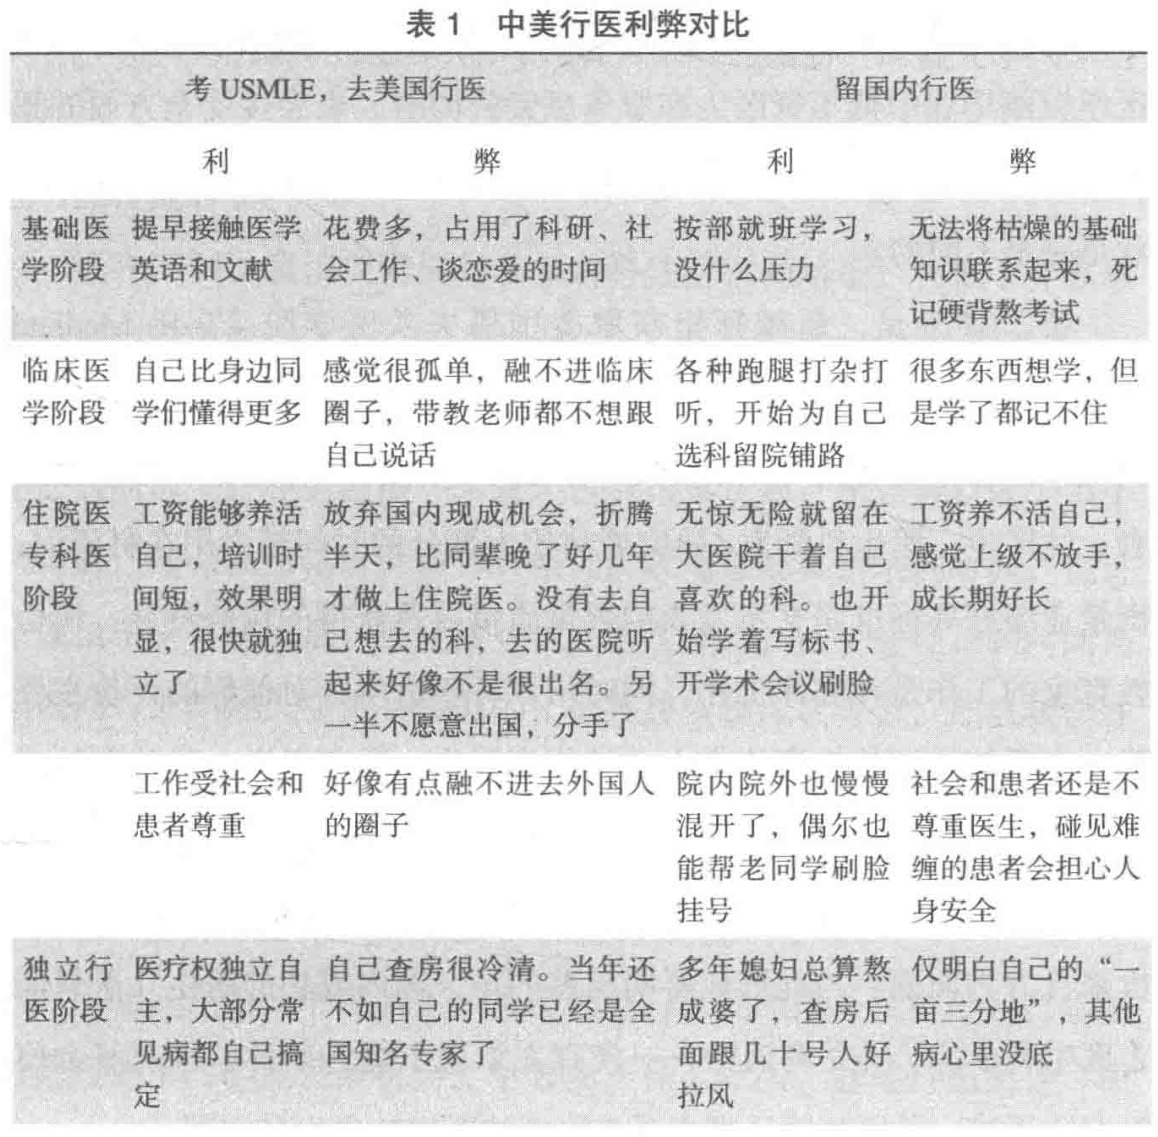
\includegraphics[width=\linewidth]{media/image2.png}
    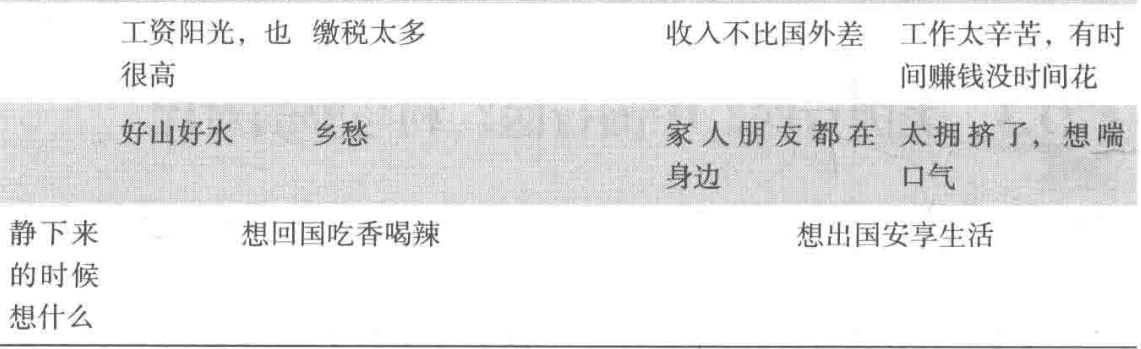
\includegraphics[width=\linewidth]{media/image3.png}
    \caption{中美行医对比}
    \label{fig:compare}
\end{figure}

在这其中,最吸引我的几点是:
\begin{enumerate}
\item 对于科研,想做就做,不想做就不做,没有人强迫您。是否做科研也不会对职业发展产生影响。
\item 有较好的work life balance,有时间享受生活(如内科hospitalist,上7天休7天)
\item 工资阳光,属于中产的中上层
\end{enumerate}
\subsubsection{FAQ}
\begin{enumerate}
    \item \textcolor{red}{Q:}参加USMLE考试(以下简称“考U”)需要什么条件?

A:在MATCH前,临床医学本科毕业即可。

\item \textcolor{red}{Q:}考U需要硕士/博士/博士后吗?

A:完全不需要。考U中有一个很重要的概念即YOG(Year of graduation),住院医项目倾向于毕业年限较短的选手。也就是说,如果您本科毕业就立刻去MATCH的话,YOG=0,是一个很大的优势哦(当然考试和推荐信也要有)!但是,如果您有志于赴美行医的同时从事科研,准备去面试大学附属/教学医院的住院医项目的话,那么上个硕士/博士,多发一些文章,说不定也是个优势。

\item \textcolor{red}{Q:}考U需要花多少钱?

A:大概总共30万人民币左右,但不需要一次性交完,一两年内陆陆续续花的。

\item \textcolor{red}{Q:}考U需要花多长时间?\label{mark-4.}

A:时间确实因人而异,我估计到MATCH需要两年吧。Step1(一年)${\rightarrow}$Step2 CK(6个月)${\rightarrow}$临床实习(6个月)${\rightarrow}$Step3(1个月)${\rightarrow}$MATCH(住院医师,根据科室而定,内科3年)${\rightarrow}$主治医师

\item \textcolor{red}{Q}:美国住院医/主治医生收入怎么样?

A:住院医(年收入),见\ref{fig:resident};主治医生(年收入),见\ref{fig:attending}
\begin{figure}[htbp]
    \centering
    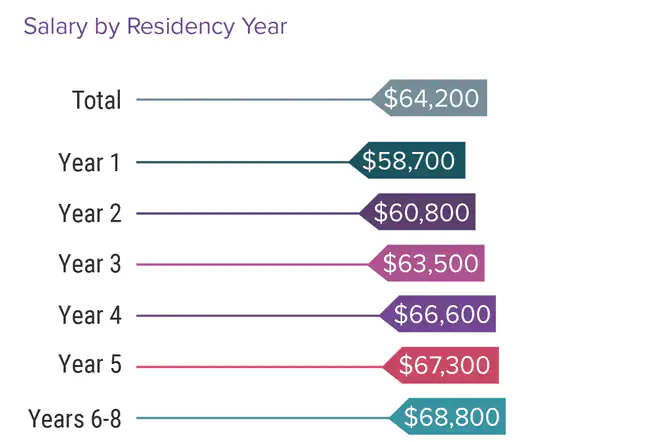
\includegraphics[width=\linewidth]{media/image4.png}
    \caption{住院医(年收入)}
    \label{fig:resident}
\end{figure}
\begin{figure}[htbp]
    \centering
    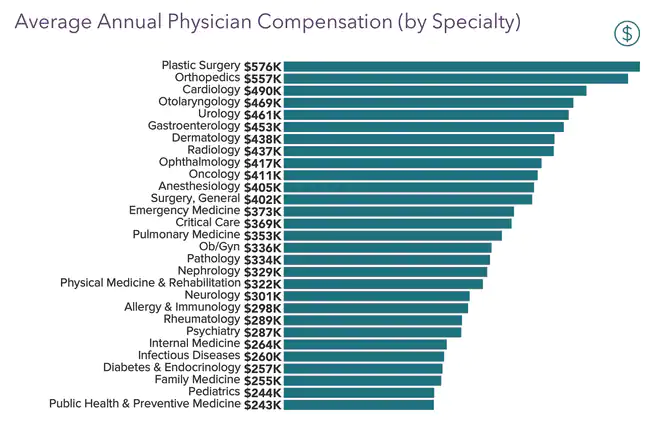
\includegraphics[width=\linewidth]{media/image5.png}
    \caption{主治医生(年收入)}
    \label{fig:attending}
\end{figure}
\end{enumerate}
\subsubsection{进一步了解}

\paragraph{公众号}
\begin{enumerate}
\item 百歌医学(推荐程度${\bigstar}$${\bigstar}$${\bigstar}$${\bigstar}$${\bigstar}$)
\begin{enumerate}[]
\item 微信公众号${\rightarrow}$加入考U群
\item 《赴美行医:故事、观点和指南》:\textbf{必看!必看!}帮您全方位了解考U的组成和学习方法。
\begin{theorem}
    其中有部分内容已经过时,如Step1 已改成pass/fail制,不需要准备很长时间(补充:虽然p/f了,但有一定可能Match系统还是能使用你的成绩的,这个没有定论,可以选择信或不信。);Step2 CS已取消,以OET代替。
\end{theorem}
\item 百歌会推荐他们的精讲课程,不推荐看这个。贵而且质量不如外国的课。
\end{enumerate}
\item 满逗逗的深夜食堂(推荐程度${\bigstar}$${\bigstar}$${\bigstar}$${\bigstar}$${\bigstar}$)
\begin{enumerate}
\item 已经当上主治的前辈,有ta个人的经验
\end{enumerate}
\item 夏可医学(推荐程度${\bigstar}$${\bigstar}$${\bigstar}$${\bigstar}$${\bigstar}$)
\item Shanghai USMLE Group,有一些经验分享会和考经
\item 知行和医USMLE(推荐程度${\bigstar}$${\bigstar}$${\bigstar}$${\bigstar}$${\bigstar}$)
\item 很优秀的清华八年制前辈,马上要麦外科
\end{enumerate}
\paragraph{学习资源}


\begin{enumerate}
\item \href{https://afratafreeh.com/\#tdsub}{AfraTafreeh {\textbar} Free Content For Medical Students}
\begin{enumerate}
\item 非常多的课程和书籍
\end{enumerate}

\item \href{https://en.imedicaldoctor.net/}{IMD}
\begin{enumerate}
\item 集齐众多题库和课程资源,40\$/y
\end{enumerate}

\item \href{https://dr-notes.com/\#tdsub}{Dr Notes - Ebook Library}
\begin{enumerate}
\item 非常多书籍、笔记
\end{enumerate}

\item 学长的\href{https://www.h4rvey.com/}{考u个人网站}
\end{enumerate}
\paragraph{其他了解途径}

小红书、微信讨论群(mitbbs等)、一亩三分地、reddit

\subsection{加拿大行医(口腔)}

加拿大医学学位和美国一样,都属于本科后教育,都需要先获得通识类本科学位,至于获得行医资格。
\subsubsection{大致步骤}
\begin{enumerate}
\item 参加通识考试 AFK(Assessment of Fundamental Knowledge)
\item 报考并准备 ACJ (Assessment of Clinical Judgement)和ACS(Assessment of Clinical Skills) (AFK,ACS和ACJ同属于一类考试(Equivalency process)中的三步,三步缺一不可。这三步考完之后,考生会拿到一个Equivalency process passed certification。)
\item  考过这个Equivalency process的考生,NDEB会自动帮考生获得written exam和OSCE的考试资格。NDEB会寄给考生一张NDEB certification。证明该牙医有资格成为加拿大范围的合法牙医了。
\end{enumerate}
\begin{theorem}
    但是想要获得行医资格,\textbf{大前提都需要先获得永久居民PR} 。
\end{theorem}


参考一下印度留学生的路径:在印度读了的牙医本科同学,申请到加拿大牙学院读一个master(一个master班里有一半是印度同学),学法语,2-3年后毕业申请移民,考NDBE考试,这样身份和执照考试两个问题都解决了,就可以在加拿大行医了,这也是一条经过很多印度同学证实可行的路。所以McGill 的master项目每年都有很多印度留学。

具体的详细申请 我可以放一些链接 供大家参考

\href{https://mbd.baidu.com/ma/s/1TDlTG3E}{https://mbd.baidu.com/ma/s/1TDl6TG3E}

\url{https://weibo.com/ttarticle/x/m/show\#/id=2309404857469091577934&_wb_client_=1?s_trans=3720409971_&s_channel=4}
\section{如何写简历}
\begin{itemize}
\item 模板:学校有与\href{https://cv.qiaobutang.com/school/sign/wechat}{乔布简历}合作;英文简历推荐overleaf.
\item 首先大量观看其他优秀简历,xhs或其他平台有很多真实简历,进行扫盲;不需美观,黑白简洁即可。
\item 从上到下,基本结构为简单个人信息,教育经历,发表文章,科研/实习经历,社团/课外经历,技能证书奖项。
\item 各项经历需要突出自己的贡献,学会用数字量化,利用\textbf{STAR法则}(建议谷歌搜索,详细学习)清晰讲述自己从这段经历的收获。
\item 修改简历:我可以帮助简单修改简历,免费的话仅限女性,我的联系方式在结尾;或者寻求学校就业老师进行简历修改;关注或参与仙交职协社团,偶尔会有简历修改活动。
\end{itemize}
\chapter{特别篇(1):润出医学部}

医学学弟学妹们好,为了帮助大家更好地了解并完成入学选拔,我们特此定制了一份简易的新生选拔白皮书。

我们人为的把选拔学院分为:未来技术学院、钱院、越杰与人工智能。并从这些学院中寻找到了一些学长学姐,征集了他们关于学院与选拔的想法。

注意,以下所有的内容皆为一家之言,不官方也不严谨。我们指导,获取信息的最好方式是兼收并蓄,建议各位同学遍读百家,然后做出自己的决定。

\section{钱-计试}

\subsection{学院介绍}

\begin{enumerate}
	\item 师资力量
	      	          
	      配备一流的教学条件、聘请一流的教师、选用一流的教材,实行国际化教学模式。
	      	          
	\item 培养方案
	      	          
	      强化科研训练。为每位学生配备学业导师,对学生的学业与科研训练进行一对一的培养。从三年级开始将学生分至相关方向,除继续学习有关课程外,参加由导师领导的研究生讨论班,协助参与部分研究工作。加强国际交流。从国内外聘请著名教师为试验班学生讲授基础主干课程;聘请国内外著名专家学者为试验班的学生进行讲座和座谈。
	      	          
	      方案可以在入学后登录\href{http://ehall.xjtu.edu.cn}{西安交通大学教务办事服务大厅}查询。计试的方案相对普通计算机会少很多杂课。
	      	          
	\item 学校支持
	      	          
	      选送优秀学生到国(境)外知名高校学习相关基础课程和专业课程。学习时间分为暑期学校(一般为6周), 一学期和两学期。交大认可在国(境)外高校取得的学分。选送方式为学校安排和学生自己联系相结合。学校为选送学生提供相应的奖学金(含交通费用、学费和资料费),并负担部分生活费。(具体根据《西安交通大学基础学科拔尖学生培养试验班学生赴国(境)外学习管理办法》的相关规定执行。)
	      	          
	      学校给予计试的支持可以算是相当丰厚的了。在出国留学方面,书院鼓励学生出国,访学交流的费用报销很高,基本可以出国交换不用自费。在国内升学方面,计试有比较高的保研倾斜,前几届计试基本都是全员保研,而计试每年又有不少同学出国升学或者就业,甚至有保研指标溢出的情况出现。本科期间,计试学生有更多机会在低年级进入本校老师的课题组进行科研尝试,训练学术技能。
\end{enumerate}

\subsection{专业介绍}

\begin{enumerate}
		
	\item 班级情况
	      	      
	      班级大概有四十多名学生试验班的学生培养实行分流制。主要是针对学无兴趣和学习能力不足的学生进行分流。如规定的本科必修课程中有不及格者或一年所修的专业主干课程中有3门次以上(含3门次)的课程成绩为70分以下者将分流到原专业或理学院内其他相关专业。(具体根据《西安交通大学“基础学科拔尖班”学生管理规定(暂行)》的相关要求执行)。
	      	      
	      计试全名为计算机试验班,在报名时专业名称为计算机科学国家拔尖计划(计算机H)。计试一般每年高考招生15个,少年班10个,大一入校选拔15个,总共四十人,经过大一大二两年淘汰之后剩下三十人,其中会在大一结束时继续补录。
	      	      
	\item 保研政策
	      	      
	      试验班的学生本科毕业时,学校对于这些学生保送我校读研究生的指标予以倾斜,对于其中特别优秀者,学校将推荐到国外著名大学继续深造。
	      	      
	      计试并没有像钱班那样有“全员保研”的承诺,但计试有比较大的保研倾斜。前几届计试基本只要不被淘汰就可以全员保研。而且计试的学生出路选择相对多元,每年出国升学,本科毕业工作的同学不在少数。
	      	      
	\item 竞争压力
	      	      
	      真的非常大但不得不说,想要提升自己的能力没有痛苦的蜕变就不会有让人满意的结果,比如第一步先要保证不能被淘汰出去。
	      	      
	      计试是西交计算机专业,在科学技术方面最好的班,计试同学普遍比较刻苦(或者卷度较大)。由于计试人数更少,因此班内同学的竞争压力也远大于大类。例如22级学分绩在大类可以排名至前百分之十五的同学, 在同级计试只能排到百分之六十。
	      	      
	\item 就读体验
	      	      
	      就读体验在一个真正可以提升自己能力的班级里,即使压力大,却也收获颇丰。
	      	      
	      计试有专门主管教学的老师。唐老师亲自修改计试的培养方案,删掉了很多杂课,在大一就加入不少专业 课,所以整体体验下来,计试的学习相对压力更大,但是学习内容也更加充实,不必再做很多无用的内卷。同时计试的辅导员(所有不同届的计试辅导员都是一位老师)十分给力,会经常慰问学生,了解情况,心理压力等等都可以随时和辅导员沟通。同时因为计试有别于普通行政班的特殊性,日常交流学业或技术问题更加方便,班级内部凝聚力和学术氛围比较强。
	      	      
	\item 对比(与普通班)
	      	      
	      \begin{enumerate}
	      	\item 保研情况
	      	      	      	      
	      	      前几届全部保研,最近是按比例,比例挺大一半以上了至少,肯定是比普通班好很多的。
	      	      	      	      
	      	      西安交通大学计算机专业(不加计试)的保研率大约为0.2至0.3。计试最近几年都是全员保研(除个别人)。去向方面,普通计算机类一般没有出国,外保大约10人,可以保研至清北华五大约五人。计试最后三十人近两年直接就业较少,留在本校约二十人,保研至上交清华浙大5\textasciitilde{}7人,申请QS前五十大约五人。
	      	      	      	      
	      	\item 培养方案差异
	      	      	\begin{itemize}
	      	      	    \item 2022届普通版还要学大化工图,这个计算机试验班就不学。但今年好像普通班也改了,但总的来说还是这个班培养方案更精简一些吧。
	      	      	      	      
	      	      \item 课内学业方面,在大一大电类的同学可能会接触到若干无用而且可能压分的课程--工图,大化,生物和大计等等。其中尤其是工图,很多同学在工图上耗费时间非常多,但是工图成绩普遍偏低。计试在大一没有这些课,大一上的大计换成程序设计,大一下的课程换为离散,数据结构和计导。
	      	      	      	      
	      	      \item 在后续课程中,计算机普通班需要学习三门电路课,而计试则将数电模电二合一,总共两门。总体来看,计试的培养进度较普通计算机快了半年,其中少了一些杂课。从四年课程上来看,差别不明显。
	      	      	\end{itemize}      	      
	      	      
	      \end{enumerate}
\end{enumerate}
\subsection{选拔情况} 
\begin{enumerate}
	\item 笔试
 \begin{itemize}
     \item 数学和英语2022年数学是高中内容(有几年出的题是大学内容的题),英语和四级类似。
	      	      
	     \item  选拔笔试就是入学的数学英语考试。其中数学以高中知识为基础,基本没有超纲题,有少量经典高数例题, 数学备考建议先看一看高数教材(同济版或交大自用的工科数学分析),练手可以参考往年高中数学联赛一试题。
	      	      
	     \item  英语题型与高考有很大不同,与四六级有些许类似。大家要先准备好收音机(考试通过收音机放听 力),其次多练习下英语写作,考试时作文书写量比较大。本次英语考试的成绩也会决定英语分级情况。
 \end{itemize}
	      
	      	      
	\item 面试
	      \begin{enumerate}
	      	\item 面试模式
	      	      	      	          
	      	      笔试之后大约选拔出60人,通过最后的面试选拔15人。五位老师一次面五个人。
	      	      	      	          
	      	\item 面试问题
	      	      	      	          
	      	      英语问答,数学能力测试,询问奖项。
	      	      	      	          
	      	      计试面试形式很像自招时代的面试。22级选拔的面试流程大概如下:
	      	      \begin{enumerate}
	      	      	\item 五个人一组,进面试教室。
	      	      	\item 老师共有五位,其中一位老师主持面试。
	      	      	\item 首先五个人依次用英语回答一位老师的提出的问题(每个人问题不同)
	      	      	\item 接下来五个人依次抽取一道题目作答,作答前有大概三分钟时间思考/计算(提供草稿纸和笔)。思考完毕之后随时可以举手作答。
	      	      	\item 最后主持的老师会依次询问一些涉及计算机科学的其他问题。
	      	      \end{enumerate}
	      	      	      	          
	      	      主要面试环节到此结束,在走之前老师会再次登记每个人在高中获得的数理竞赛奖项,如果是信息奥赛方面的奖项老师可能会和你聊一会。 以我本人为例,我当时抽到的几个问题回忆如下:
	      	      \begin{itemize}
	      	      	\item 英语问题:Your opinion about the difference between cs and ai?
	      	      	\item 抽到的问题:\href{https://blog.csdn.net/lzq603/article/details/110092371}{红军协同对抗蓝军问题},问题本质还是信息安全。
	      	      	\item 最后询问的问题:在你眼中计算机科学的意义?
	      	      \end{itemize}
	      	      根据回忆,其他同学抽到的问题类型非常多,有的同学抽到的是计算题,但无论什么题型,本质还是计算机科学的某一具体领域。
	      	      	      	          
	      	\item 面试注意事项
	      	      \begin{itemize}
	      	      	\item 大方自信即可。
	      	      	\item 注意衣冠整洁,朴素大方。
	      	      	      \begin{theorem}
	      	      	      	一定不要迟到!具体到面试当天可能时间会稍微延迟,但是绝对不要迟到。
	      	      	      \end{theorem}
	      	      	\item 英语作答时要勇于发音。虽然大家学的英语大部分都是哑巴英语,但在面试现场如果因为怯于发音而不敢作答是很大的减分项!有时间的同学暑假可以先学学雅思/托福。
	      	      	\item 语速放慢,用心作答,切忌嘴巴比脑子转的快。
	      	      \end{itemize}
	      \end{enumerate}    
	      	      
	\item 心得体会 
	      \begin{itemize}
	      	\item 准备心得
	      	      	      	              
	      	      只要认真准备数学英语做一做题目熟悉一下就可以,面试尽可能展示自己的优势即可。
	      	      	      	              
	      	\item 就读心得
	      	      	      	              
	      	      大学和高中的学习模式生活模式都会发生很大的改变,但只要肯努力,找对方法,就可以获得自己能力提升的满足感和踏实感。
	      	      	      	              
	      	      面试选拔的意义在于弥补笔试选拔的不足--考察学生的表达能力以及对未来在本专业发展的最基本构想。因此大家准备面试首先需要补充自己对计算机科学的基础认识(如果是从未系统接触过computer science的同学,可以从这门\href{https://www.bilibili.com/video/BV1EW411u7th/}{科普课}入手
	      	      	      	              
	      	\item 其次,大家要开始将自己的心态从高中生转向大学生,勇敢的表达观点并跟上面试官的思路。尤其是英语口语,大家一定要注意多加训练,一口流利的英式英语与清晰的思路可以护送你通过面试。
	      \end{itemize}
\end{enumerate}
\section{钱-能动}

\subsection{学院介绍}

\begin{enumerate}
	\item 师资力量
	      	      	          
	      能动学院师资力量比较丰富,有3名院士,研究方向很多。新生入学会分配学业导师,一学期可能有一两次谈话。
	      	      	          
	\item 培养方案
	      	      	          
	      大一通识教育,大二通识教育+专业课(流体力学、工程热力学),大三专业课(传热学等)。
	      	      
	      	      	          
	\item 学校支持
	      	      
	      有许多重点实验室,还有专业相关竞赛。分专业前学院会组织讲座、领导面对面咨询活动。
\end{enumerate}

\subsection{专业介绍}

\begin{enumerate}
			
	\item 班级情况
	      \begin{itemize}
	      	\item 人数:22级每个钱班大约40人,每班分配1个班主任
	      	      	      
	      	\item 来源:少年班、高考录取、入学选拔(22年入学选拔每个钱班15人)
	      	      	      
	      	\item 辅修:大一结束会选择辅修专业(三选一),辅修课程大三会上,毕业后会有荣誉证书。如果要拿辅修学位证,需完成辅修专业毕业设计。    
	      \end{itemize}	      
	        	      
	\item 保研政策
	      	      	      
	      全保研,前提是不被淘汰(3门低于70分/挂科),淘汰则与大类一起分流。
	      	      	      
	\item 竞争压力
	      	      	      
	      总体比较卷,均分、竞赛、科研、志愿、入党各个方面都有竞争,但也有个体差异。因为钱班学的课程比较多比较杂,所以压力会大一些。
	      	      	      
	\item 就读体验
	      	      	      
	      特色课程和综合工程训练挺有意思的,比如音乐课、陶艺课、3D打印。但部分基础课程感觉课时紧,学的内容比较多。像是化学原理这门课,半个学期学大化,半个学期学有机;程序设计也是在半个学期上完。
	      	      
	      钱院还有一些隐性福利。比如有自己的答疑群,考前会组织讲座、答疑、帮扶,个人认为很有帮助,还能认识厉害的学长学姐;有组队背单词、学习伴侣等活动;出国交换能报销部分费用;女生住在彩虹楼等。
	      	      	      
	\item 对比(与普通班)
	      	      	      
	      \begin{enumerate}
	      	\item 保研情况
	      	      	      	      	      	      
	      	      全保研,前提是不被淘汰(3门低于70分/挂科),淘汰则与大类一起分流。
	      	      	      	      
	      	      保外校比大类难,因为名额较少,内部竞争激烈。
	      	      	      	      	      	      
	      	\item 培养方案差异
	      	      \begin{enumerate}
	      	          \item 大一的基础课程(高数、线代、工图、大化、大物、程序设计)四个钱班一起上;公共课程(近代史、德 法、国防教育)是两个钱班一起上;英语课大一上是本班小班授课。以上课程的老师是分配好的,不需要抢课。英语大一下要选课(如托福强化、国际演讲、学术写作等)。工图、英语、大化、程设这些科目和大类的培养方案及考试内容不太一样(如大化是把大学化学和有机化学合在一学期上),高数、线代、大物、近
	      	      	      	      
	      	      \item 代史、德法、国防教育和大类考试是一样的。英语四级是大一上考,大类好像只有a班是大一上考四级。此外钱班大一下还有化学和物理实验。总体来说,课程安排更紧凑,要学的内容更多。
	      	      	      	      
	      	      \item 大二也上基础课程,但钱班大二没有英语课;需学一门社科类课程(四选一);大二下会涉及专业课。大三会上专业课及辅修课程。
	      	      	      	      
	      	      \item 通识课本科四年只用选两门,大一上钱班还会学特色课程(音乐/建筑/陶艺三选一)。大一两学期都有综合工程训练(机类和电类各选1门,在周末上,为期两周或四周)。
	      	      \end{enumerate}	      	      	      	      
	      	      
	      \end{enumerate}
\end{enumerate}
\subsection{选拔情况} 
\begin{enumerate}
	\item 资格审查
	      主要看高考成绩,以及竞赛获奖等。
	\item 笔试
	      除开学都要考的数学、英语外,钱班还要考物理。数学往年题型不一样(真题新生群里有),22年题型与高考类似,考察高中知识。英语与四级题型类似,注意有翻译题、听力题,要自带收音机。物理22年是填空+大题,难度高于高考,去年考察了光学,建议看看所有的选修。
	      	      	      
	\item 面试
	      \begin{enumerate}
	      	\item 面试模式
	      	      	      	      	      	          
	      	      去年钱班面试分为英语素养,科学素养,人文素养三部分,五人一组坐一排,面对若干老师。
	      	      	      	      	      	          
	      	\item 面试问题
	      	      	      	      	      	          
	      	      英语是做自我介绍(1min左右),老师会根据自我介绍的内容用英文提问。科学素养是每个人抽一道题,题目与生活较贴近,考察物理化学知识。比如:冲泡速溶饮料是先加水还是先加粉?老师可能根据回答追问。人文素养考察时事政治,比如:终南山违建别墅、“七有五性”是什么。
	      	      	      	      	      	          
	      	\item 面试注意事项
	      	      \begin{itemize}
	      	      	\item 要提前准备英语自我介绍(我还准备了为什么报考这个专业及这个学院、自己报考的准备与优势、对本专业的了解、西迁精神等话题)。注意仪容仪表、语气眼神,尽量表现得自信大方。
	      	      	\item 人文素养可能会考察到盲区(比如我就考了“七有五性“),老师会逐步引导你,尽量表现出对时事的了解与政治素养。
	      	      \end{itemize}
	      \end{enumerate}    
	      	      	      
	\item 心得体会 
	      \begin{itemize}
	      	\item 报考前建议找学长学姐了解钱班的利弊,比如钱班保外会比大类困难,学的内容很多。同时可以了解下这个专业的研究方向、就业前景,上专业所在学院官网(比如西安交通大学能源与动力工程学院)了解专业培养方案。钱班培养方案会有不同,具体可以找学长学姐咨询。
	      	\item 建议暑假背4级单词,保持英语语感,如果大一上考四级则有优势。
	      	\item 扩展信息渠道,多上教务处官网了解比赛、出国交换信息,也可以进一些咨询群(许多信息老师不会发到班群里,需要自己搜集,否则跟别人会有信息差)。
	      	\item 可以接触下腾飞杯、数模竞赛等,就算没拿奖也能为以后参加积累经验,对未来方向确定也有帮助。
	      \end{itemize}
\end{enumerate}

\section{钱-物理试验班}

\subsection{学院介绍}
西安交通大学物理学院前身为始建于1928年的交通大学物理系,1930年并入交通大学科学学院。1952年因院系调整,物理系改为物理教研室。1956年随校整体迁至西安。1984年重建物理系。2020年成立物理学  院。

在近90多年的办学历史中,学院汇聚和造就了以裘维裕、赵富鑫、殷大钧、胡刚复、叶蕴理、周同庆、方俊鑫、吴有训、程守诛、吴百诗等为代表的一大批在国内外享有极高声誉的教育家。学院坚持“基础课程教学一流、基础科学研究一流”的发展理念,以科教融合、创新发展、造就引领未来物理专业拔尖创新人才为宗旨,为国家培养了大批优秀人才。 物理学(国家拔尖计划)是2009年首批进入国家“基础学科拔尖学生培养试验计划”的人才培养基地之一,突出“理工交融、潜心基础、勇攀高峰”的拔尖人才培养特色,目前已招收了14届学生。

\begin{enumerate}
	\item 师资力量
	      	      	          
	      学院现有教职员工160人,其中教授43人,副教授57人,国家级万人名师1人,国家级领军人才3人,优秀青年基金获得者4人,其他国家级青年领军人才4人,教育部“跨世纪优秀人才培养计划”2人,教育部“新世纪优秀人才”6人,教育部全国高校教指委委员3人,省级教学名师4人,陕西省各类人才20余人;工程技术人 员21人(含高级工程师9人),行政人员9人。
	       	          
	\item 培养方案
	      \begin{enumerate}
	      	\item 科学选拔,动态管理
	      	                
	      	      每年招收50名左右学生,分别从高考生、少年班学生及各专业优秀生中选拔,通过“笔试、面试”两个阶段,和“特色笔试、数理思维、人文素养、创新潜能”四个模块,考查学生科研兴趣、学习天赋、创新潜质等素养。实施动态评估,建立差异化的进出机制。
	      	      
	      	\item 理工交融,个性化培养
	      	      
	      	      结合学校优势工科,设置工程基础课程模块、交叉学科选修模块。鼓励学生跨学科、专业进行基础知识学 习,进入各国家重点科研平台,完成创新实践培养环节。制定了灵活的课程免修、缓修、及补修制度,试行完全学分制。高年级学生允许跨专业修读专业课程,允许优秀学生提前选修物理专业研究生课程。实施暑期小学期制,进行学科竞赛、短期国际暑研,国外专家短期授课或讲座等。
	      	      
	      	\item 汇聚名家,打造一流师资
	      	      
	      	      试验班瞄准顶尖教育,集合优势资源,汇聚名师大家,为学生进行小班授课,实施个性化培养。长期聘请来自北京大学等国内顶尖高校的国家教学名师和知名教授担任试验班专业主干课程主讲;聘请我校外籍教授、及国家/省级教学名师等讲授核心课程。从大二开始为学生配备优秀科研导师,进行学业指导和科研训练。每年邀请诺贝尔奖得主、两院院士等国内外知名学者定期来校为试验班学生讲座、座谈,参与人才培养。
	      	      
	      	\item 双院双导师制,国际化培养
	      	      
	      	      试验班以“教学特区”的方式进行管理,体现因材施教。基于“学院+书院”双院制,实施灵活管理政策,突破常规模式。学生管理实行导师制与班级管理相结合,一对二配备指导教师:学业导师指导学生学习规划和志趣培养;科研导师带领学生进入前沿课题研究。与美国加州大学伯克利、圣母大学等10余所国际名校签订联合培养学生协议,遴选、资助学生前往国外进行为期一学期至一学年的学分互认课程学习,参与科研合作交流。
	      	      
	      	\item 力推科研训练,塑创新能力
	      	      
	      	      构建实践培养体系,打造创新实践平台,围绕学生综合素质和学术创新能力等核心要素,开展多样化、多层次的科研训练。试验班学生积极参加国内外学科竞赛、大学生数学建模、挑战杯等课外学术竞赛等,多次获得全国团队特等奖、一等奖以及国际、国内的各类个人奖项。近五年,试验班学生本科在校期间已在Phys. Rev. Lett、Phys. Rev.系列及Nature子刊发表高水平SCI学术论文50余篇, 承担国家级“大学生创新训练项目”40余项。
	      \end{enumerate} 	          
	      	              
	\item 学校支持
	      	      
	      学校比较重视对试验班学生的培养。
\end{enumerate}

\subsection{专业介绍}

物理学(国家拔尖计划)是2009年首批进入国家“基础学科拔尖学生培养试验计划”的人才培养基地之一, 突出“理工交融、潜心基础、勇攀高峰”的拔尖人才培养特色,目前已招收了14届学生。

“基础学科拔尖学生培养计划”是国家教育体制改革试点项目,旨在培养基础知识扎实、专业知识出众、科研思想活跃、国际视野开阔、发展潜力明显,未来成长为相关基础学科领域的领军人物,并逐步跻身国际一流科学家队伍。
\begin{enumerate}
			
	\item 班级情况
	      	      	      
	      分两个班级,每个班约25人,两个班的专业课基本是一起上的。
	      	      	      
	\item 保研政策
	      	      	      
	      不确定,疫情后因为出国受阻,有几届是全保,但是从22届以后就不是全保了,每一届的保研政策不确定,但是保研率会比普通大类高。
	      	      
	\item 竞争压力
	      	      	      
	      相对钱班和其他几个试验班,竞争压力较小,除非没好好学,不太容易被淘汰,保研也比较容易。
	       	      
	\item 就读体验
	      	      	      
	      暂无。
	      	      	      
	\item 对比(与普通班)
	      	      	      
	      \begin{enumerate}
	      	\item 保研情况
	      	      	      	      	      	      
	      	      保研率远高于普通班。
	      	      	      	      	      	      
	      	\item 培养方案差异
	      	      	      	      	      	      
	      	      普通班会细分专业,比如光电、理论、材料物理等,但是物试不会细分专业。物试更偏向培养物理领域的科研人才,比较注重科研。
	      \end{enumerate}
\end{enumerate}
\subsection{选拔情况} 
\begin{enumerate}
	\item 笔试
	      数学、英语题目同开学考试题,会加考物理。物理题目知识范围会涉及大学物理(比如考过多普勒效应,但是给出了公式),解题所用的数学知识基本是在中学范围内的。
	      	      	      
	\item 面试
	      \begin{enumerate}
	      	\item 面试模式
	      	      \begin{enumerate}  	      	          
	      	      	\item 5人一组,每组15分钟左右。共有5个老师进行面试,每个人依次回答面试问题,每个人的面试问题不同。
	      	      	      
	      	      	\item 首先是英语考察环节,先是一个简短的自我介绍(可能会因为时间问题取消),然后老师会用英语进行提问,你会和老师就这一问题进行交流。老师的语速很慢,并且英语占分不高,所以大家不必太过担心。
	      	      	      
	      	      	\item 接下来是专业素质考察,你会从一堆纸条里抽一个物理方面的问题,涉及力学、电磁学、光学、近代物理等,范围非常广泛。
	      	      	      
	      	      	\item 最后是一些关于个人生活的问题,这些问题都很容易回答,大家从容应对就好。
	      	      \end{enumerate}   
	      	\item 面试问题
	      	      \begin{itemize}	      	          
	      	      	\item 英语考察环节:
	      	      	      
	      	      	      问:你觉得张衡最伟大的发明是什么?
	      	      	      
	      	      	      答:一个能探测地震的仪器(相信大部分同学不会说地动仪这个单词)。
	      	      	      
	      	      	      问:请说说它工作的原理?
	      	      	      
	      	      	      答:\textasciitilde{}
	      	      	      
	      	      	\item 专业素质考察环节:
	      	      	      
	      	      	      问:从古至今,计时方式不断改进,从日晷到摆钟再到原子钟,计时精度不断提高,请问日晷、摆钟、原子钟的计时原理分别是什么?
	      	      	      
	      	      	      答: 日晷计时原理是太阳高度角会随着一天中时间的变化而变化,因此影子会随着时间移动。 摆钟计时原理是利用摆锤的周期性振动,且振动周期不变的特点,摆锤越长,振动周期越长,根据此特点可以对摆钟进行调节。 原子钟是利用了原子吸收或释放能量时发出的电磁波来计时的,这种电磁波的共振频率是不会改变的。原子种的精度可以达到每100万年误差1秒。
	      	      \end{itemize}
	      	      	      	      	      	          
	      	\item 面试注意事项
        
	      	      不要紧张,语气放平缓,一定要谦虚友好。
	      \end{enumerate}    
	      	      	      
	\item 心得体会
	       
	      如果你热爱物理,欢迎报考物理试验班。在物试的这一年里,我能深刻感受到周围同学对物理学的热爱,希望每一位进物试的同学能够在物理研究领域发挥出自己的特长,寻找到人生的方向。
\end{enumerate}
\section{人智}

\subsection{学院介绍}

\begin{itemize}	
	\item  学院、研究所简介-西安交通大学-人工智能学院 (xjtu.edu.cn)
	\item 教师-西安交通大学-人工智能学院 (xjtu.edu.cn)
\end{itemize}
\subsection{专业介绍}

\begin{enumerate}
			
	\item 班级情况
	      
	      2个班 一个班大约30人 来自高考直接分高录进来、开学选拔、少年班。
	      
	\item 保研政策
	      
	      之前听说是保研一半多人。
	      
	\item 竞争压力
	      
	      人均大佬 竞争比较激烈,90+的比比皆是。
	      
	\item 就读体验
	      
	      听说大一大二大三难度递增,笔者因为大一就很菜被吊打所以主动跑路。
	      	      	      
	\item 对比(与普通班)
	      	      	      
	      \begin{enumerate}
	      	\item 保研情况
	      	      	      	      	      	      
	      	      保研一半多人属实不错了,还有出国的一些人,保研概率其实不错。
	      	      	      	      	      	      
	      	\item 培养方案差异
	      	      	      	      	      	      
	      	      和电类比的话,大一就要学离散数学;大一难度整体不低,有代码基础的话有优势。
	      \end{enumerate}
\end{enumerate}
\subsection{选拔情况} 
\begin{enumerate}
	\item 笔试
	      \begin{itemize}
	      	\item 主要考察的是数学,英语和物理这三科首先考的是数学,如果数学没有考到前百分之50左右你就不能继续考英语和物理,如果数学考过了之后,你将会继续考英语和物理,并且面试。数学其实考了一些竞赛的题,总体难度比高考难度要大一些,但是有一些题是基础题,所以最关键的就是把能做的题做对。然后尽可能的参考一下往年的题,其实难度波动不大。
	      	      
	      	\item 英语和四六级的难度比较相似,英语主要是听力比较难,阅读是能够读懂的。作文可能会来不及写,所以建议一定要提高速度。
	      	      
	      	\item 物理考了一些概念的题,考的很多题都是基本的模型。没有涉及物理竞赛题。
	      \end{itemize}     
	             
	\item 面试
	      \begin{enumerate}
	      	\item 面试模式
	      	      	      	      	      	          
	      	      5考官面对5学生。
	      	      	      	      	      	          
	      	\item 面试问题
	      	      	      	      	      	          
	      	      面试问的和军训相关的问题,也问了英语相关的问题,还有一些科学常识和你的竞赛经历。当时我抽到的是 微波炉加热的原理。(印象中还有其他的比如问你电磁炮的原理,各种科学成果发明的物理原理)。
	      	      
	      	      面试的时候会让你先用英文进行自我介绍,然后会问一些英文的问题,比如说当时问的是怎么看待打游戏这个事情,平衡游戏和学习。
	      	      	      	      	      	          
	      	\item 面试注意事项
	      	      	      	      
	      	      钱学森书院面试的时候,通常都是五个人一队一起进去面试,然后分从早到晚很多个队。一个队里面有时候录取2个人,1个人 有时候这5个人一个都不会被录取。面试占比百分之50,所以重在面试。
	      	                    
	      	      \begin{example}
	      	      	建议面试的时候不必纠结,多抢答问题展现积极态度(但是当时一起来的据说有的人一个题没抢也被录取了的,有的道道都抢但是乱答寄了)所以尽可能分析问题而不是编答案可能比较好(?)
	      	      \end{example}
	      	      
	      \end{enumerate}    
	      	      	      
	\item 心得体会 
	      \begin{itemize}
	      	\item 大一时候这个专业60多人,现在大三了还剩40多人在里面(细品)。\href{https://www.zhihu.com/question/368080680/answer/2993647435}{知乎回答}大多数比较片面,仅供参考。
	      	\item 总的来说人智大佬云集,如果你本就很牛,那么在里面一定会如鱼得水、大有作为。
	      	\item 里面的同学都非常优秀且努力,氛围其实很棒,也有很多少年班的大佬、科研大牛、超级卷怪(doge),可以给你带来好的影响。
	      \end{itemize}
\end{enumerate}
\section{未来-医工}

\subsection{学院介绍}
未来技术学院以“未来科技牵引、学科交叉支撑、产教融合驱动、开放探究教学”为建设理念,作为学校创新人才培养模式的“试验田”,探索构建多元驱动式贯通制一体化的跨界融合人才培养新模式。

\begin{enumerate}
	\item 师资力量
	      	      	          
	      组建校企合作“双师型”导师队伍,构建前沿性、前瞻性的课程体系,实施项目驱动的自主式、研讨式、探究式教学方法。以基础医学、临床医学教学团队教师为主体,以及中科院近代物理所、西部超导材料有限公司等国内知名研究机构和企业专家加入教学团队。促进产教融合。医工学团队由西安交大副校长、一附院院长吕毅教授担任责任教授,在刘昌、张明、赵永涛、仟正、吴荣谦、杨健、吴春生、郑彦臻、张德文、李虞锋、徐光华、樊林、高水平师资团队。
	      	      	          
	\item 培养方案
	      	      	          
	      五年制,目前老师说会发医学学位+个人选择的小方向工学学位证(该说法存在争议,但至少是医学学位   证),前两年基础课程,包括高数大物等,之后会学医学知识,包括解剖,分子与细胞等等课程,也会学习医学影像学这些课程。每周固定时间会到一附院或者实验室进行实地上课,并完成实验报告。
	      	      
	      	      	          
	\item 培养目标
	      	      
	      培养高素质医工交叉复合型人才,全面解决"医学需求和工业技术的不匹配,医生和工程师的沟通不通畅"的问题,发展新型的物理诊疗技术、设备及方案 改变固有的诊疗模式,培养具有完备的医学基础知识、能够与工程师无障碍沟通。
\end{enumerate}

\subsection{专业介绍}

\begin{enumerate}
			
	\item 班级情况
	      	      	      
	      医工这个方向专业为十个人。
	      	      	      
	\item 保研政策
	      	      	      
	      目前说是只要大一不低于两门70都保研。
	      	      	      
	\item 竞争压力
	      	      	      
	      由于每个人在之后学习过程中会有感兴趣的小方向,所以说十个人有可能读出来会有好多小方向,所以只需要在自己选择的路上好好学就可以了,竞争压力比其他专业小很多。
	      	      	      
	\item 就读体验
	      	      	      
	      我们可以和上一届的学长学姐们一起参与到他们的大创腾飞杯等比赛当中,所以互相交流,十分方便。另外,我们的专业课师资充裕,有一门实践课,有超过十个老师为我们轮流上课,分别介绍他们的研究方向。
	      	      	      
	\item 对比(与普通班)
	      	      	      
	      \begin{enumerate}
	      	\item 保研情况
	      	      	      	      	      	      
	      	      对比于普通班来说,保研难度大大降低。
	      	      	      	      	      	      
	      	\item 培养方案差异
	      	      	      	      	      	      
	      	      比较大,因为这是一个医学和工学的结合,所以说学的内容还是比较多的,而且需要自己选择好自己的方向,在自己感兴趣的领域内不断深钻。
	      \end{enumerate}
\end{enumerate}
\subsection{选拔情况} 
\begin{enumerate}
	
	\item 笔试
	      22年是笔试大概70个人,面试只去了30个左右有些人退出了,最终选出十个。
	      	      	      
	\item 面试
	      \begin{enumerate}
	      	\item 面试模式
	      	      	      	      	      	          
	      	      面试的模式是由五个老师,然后面试一个学生。进去之后一分钟的英语自我介绍,然后抽一套题回答问题,这些问题有人文方面的问题主要是传统文化文言文解读。
	      	      	      	      	      	          
	      	\item 面试问题
	      	      	      	      	      	          
	      	      \begin{enumerate}
	      	      	\item 知识方面的问题,会让你在三分钟内解决一道题。
	      	      	\item 常识性问题比如你的优势,缺点,为什么想加入本专业?
	      	      \end{enumerate}
	      	      	      	      	      	          
	      	\item 面试注意事项
	      	      面试注意自信,不要慌张即可。
	      \end{enumerate}    
	      	      	      
	\item 心得体会 
	      \begin{itemize}
	      	\item 在这里,师资力量比较充足,鼓励学生积极参与创业创新活动,投身到比赛当中去,学长学姐们也会耐心的帮助你,老师们也都很善解人意,尽量满足大家的需求。
	      	\item 但是对个人而言,想学好这个专业,就要先学好医学。如果自己对医学有恐惧心理,则不建议报考。
	      \end{itemize}
\end{enumerate}
\section{越杰-材料}

\subsection{学院介绍}

\begin{enumerate}
	\item 师资力量
	      	      	          
	      能动学院师资力量比较丰富,有3名院士,研究方向很多。新生入学会分配学业导师,一学期可能有一两次谈话。
	      	      	          
	\item 培养方案
	      	      	          
	      大一通识教育,大二通识教育+专业课(流体力学、工程热力学),大三专业课(传热学等)。
	      	      
	      	      	          
	\item 学校支持
	      	      
	      有许多重点实验室,还有专业相关竞赛。分专业前学院会组织讲座、领导面对面咨询活动。
\end{enumerate}

\subsection{专业介绍}
越杰这真写不出来,相当于就是有点奖学金的普通班,上课除了一些基础课和钱班一起,其他还别说真和普通班差不多,师资基础课和钱班差不多,专业课就普通班的专业课老师,培养方案和普通班没太大区别,英语课只上大一一年,会少一些,然后化学生物都要学,其他的话可能就课程顺序有点不一样,少的英语课还要多学几门其他课,如越杰材料,就要多学出国访学准备,数学物理方程,复变函数,生命科学基础等,普通班会多学有机化学,算法设计与问题解决等。
\begin{enumerate}
		      	      
	\item 保研政策
	      	      	      
	      保研要和专业所有不是钱班的一起排名竞争,但越杰班前两届保研率55\%,加上考研和出国留学,升学率有90\%。在越杰一共七个专业,只有留学奖学金评定的时候需要竞争,也就是竞争大一这一年,大二国庆就要评定奖学金了。
	      	      	      
	\item 竞争压力
	      	      	      
	      越杰已经毕业了两届,前两届被挂科出去或者主动退出转专业的人还比较多,每一届被踢出去的人基本上逐渐减少,2022届目前为止还没人被踢出去。	      	      
	\item 就读体验
	      	      	      
	      越杰基本上都是和专业竞争,而且退班条件是挂科,所以压力还是没那么大的。就读我是体验感很好,越杰班上同学之间联系会比普通班更多,有更多的活动,聚餐,开会,导师交流会等,班上所有人能见到的机会很多,平时上课基础课也基本上在一起,所以班上整体氛围还挺好的。
	      	      	      
	\item 对比(与普通班)
	      	      	      
	      越杰在某种意义上,就是有奖学金的普通班。学校支持就算是奖学金吧,进越杰有基础奖学金六万,每个月发1500,一年发十个月,二月和八月不发,任何科目不挂科就不会被踢出去,包括通识课,挂科被踢出去了就没这钱了,然后还有留学奖学金,最高两个人36万,最后五六个人3万,其他二十几个都是18万。
\end{enumerate}
\subsection{选拔情况} 
\begin{enumerate}
	\item 笔试
 
	      笔试数学+英语。
	      	      	      
	\item 面试
	      \begin{enumerate}
	      	\item 面试模式
	      	      	      	      	      	          
	      	      面试的话就是五个老师面试,五分钟英语自我介绍,25分钟问题回答,这部分可以用中文,用英语加分。
	      	      	      	      	      	          
	      	\item 面试问题
	      	      	      	      	      	          
	      	      没有具体需要回答的问题,会根据你前一个问题回答的方向,来提下一个问题,所以注意回答问题往自己熟悉的方向去回答,比如专业中的某一领域,某些知识你知道,那前面你就可以说你知道什么什么,然后他会紧接着问的。
	      	      	      	      	      	          
	      	\item 面试注意事项
	      	      每个问题回答充分,表达流利。
	      \end{enumerate}    
\end{enumerate}
\section{越杰-机械}

\subsection{学院介绍}

\begin{enumerate}
	\item 师资力量
	      	      	          
	      跟大类没啥太大区别,但大部分课都是指定的一个老师,且上课班级较多与拔尖班一起上,比如钱班,力试,计试,储能等(大一全年,大二上的课,除了高数和线代,别的课都是指定。其他学年还不太清楚) 当然,作为世界第一的交大机械,师资力量肯定是非常好的。
	      	      	          
	\item 培养方案
	      	      	          
	      就机械来说,课程上与大类并无太大区别(工图学的不一样)。有些课程学习时间不一样(大类大二上学化学,我们大一上就学了化学)。有一些特色课程,如表达与交流,出国访学准备。
	      	      	          
	\item 学校支持
	      \begin{itemize}
	      	\item 越杰主要的特色就是高额奖学金资助本科期间出国交流,校内校外双导师。
	      	      
	      	\item 基础奖学金6万,每个月1500(2月,8月不发),发四年。出国交流不是必须,且符合世界前50排名大学条件,短期项目(三个月以内)托福成绩达90分及以上、长期项目(三个月以上)托福102分及以上,可申请越杰奖学金项目报销。
	      	      
	      	\item 有较多机会与杰出校友近距离交流(大一期间举办过黄明生,桂生悦大佬的茶话会),且有较多班级特色的参观研学活动(参观西安港,中航西飞)。
	      \end{itemize}
	      	      
\end{enumerate}

\subsection{专业介绍}

\begin{enumerate}
			
	\item 班级情况
	      	      	      
	      7个专业,每个专业5个人。35个人均为新生选拔进入。	      	      
	\item 保研政策
	      	      	      
	      无保研倾斜,与大类学生一块竞争保研名额。
	      	      	      
	\item 竞争压力
	      	      	      
	      无保研倾斜,与大类学生一块竞争保研名额。主要是在英语上的压力较大。
	\item 就读体验
	      	      	      
	      越杰班从22届开始集中住宿,平常联系非常多,班级氛围非常活泼,班级凝聚力非常强(感触最深的就是广播体操。班里都在为共同的荣誉努力,最终也拿到了全校第一)。辅导员潘运亮很幽默,很风趣,很关心学生,能和同学们打成一片。 因为每天都是和不同专业的同学相处,无论是上课还是宿舍里,这样对于专业的了解会更全面,对于你未来的专业走向更好,其次是不同专业的同学可以更好的合作做一些项目,不需要额外去找自己不熟悉的同学。
	      	      	      
	\item 对比(与普通班)
	      	      	      
	      \begin{enumerate}
	      	\item 保研情况
	      	      	      	      	      	      
	      	      与大类竞争。有部分同学选择出国读研,随着疫情的放开,选择出国的比例肯定会大幅上升。国内学校的保研率也较高,因为大多数同学会选择本科期间出国交流半年或一年,这样在保研时导师更愿意选择你。
	      	      	      	      	      	      
	      	\item 培养方案差异
	      	      	      	      	      	      
	      	      大部分课程与大类专业相同,但会有一些必修的特色课程。比如表达与交流,出国访学准备等。大部分课程与大类没有区别,只是在学习的时间上有所不同,比如工图大类是大一上学习,而越杰班是大一下学习。其次是有少数课程越杰班要额外上的课程,大部分与出国有关,如出国访学准备,无专业课的区别。
	      \end{enumerate}
\end{enumerate}
\subsection{选拔情况} 
\begin{enumerate}
	\item 资格审查
	      报名后,会提交一个电子表格,包括你的高考成绩,竞赛成绩,社会经历等,进行初筛,来获得笔试资格。
	      \begin{example}
	      	开学考试每个人都必须参加,这个笔试资格是指如果你没有获得笔试资格,无论你开学考试成绩如何,都不纳入考虑范围。如果高考的专业是预选,那么直接获得笔试资格。然后根据开学考试的数学和英语成绩进行统一的筛选,来获得面试资格(大概会有140个人)。然后进行面试,根据综合成绩定最终人选。
	      \end{example}
	\item 笔试
	       
	      只考数学英语,全校统一试卷。进入越杰后,不管英语初始等级多少,均变为A级	      
	\item 面试
	      \begin{enumerate}
	      	\item 面试模式
	      	      	      	      	      	          
	      	      五位考官面试一个人。考官由教授和杰出校友组成。时长30分钟左右。首先用英语进行5分钟自我介绍。后续提问交流环节,不做硬性要求,中文也可。
	      	      	      	      	      	          
	      	\item 面试问题
	      	      	      	      	      	          
	      	      面试更像是在跟考官们聊天,更多的是了解个人情况。没有固定问题,基本不涉及专业知识。我去年问了一些比较正经的,比如为啥想学机械,为啥喜欢数学和物理。也问了一些比较家常的,比如喜欢哪个篮球球 星,为什么喜欢(在自我介绍中,我提到了喜欢打篮球);问我爸妈偏心我和我哥哥吗;问我和异性朋友经常交流吗,觉得异性哪些方面更吸引你。不会涉及专业问题,主要是问你的爱好,你的性格,在你的爱好领域内问一些你对它的看法,或者是你遇到困难如何面对,你如何描述你的家乡,你的父母,你受过的教育等等。
	      	      	      	      	      	          
	      	\item 面试注意事项
	      	      \begin{itemize}
	      	      	\item 看成是在与大朋友们正常交流即可,不必过于拘谨。
	      	      	\item 思路清晰,表达清楚,不要啰嗦。
	      	      	\item 举止谈吐大方,面带微笑(至少不要一脸严肃,不要把紧张都写在脸上),注意礼貌(推门进入后,可以先跟老师们鞠躬问好。起身离开时,可以再次鞠躬,说声老师辛苦)。
	      	      	\item 我去年面试的时候有个小插曲。引导志愿者听错了,让我进面试教室的时候,上一个人还没面试完。如果遇到这种情况,我觉得可以在关门的同时,鞠躬说声抱歉,不好意思。正式轮到你面试时,进去问完好之后,再对刚刚的事情致以歉意。
	      	      	\item 真诚,不要不懂装懂。不要害怕说错,要自信,因为你在他们眼睛里就是一个什么都不懂得小屁孩。如果正好碰到了面试官擅长的领域,你说错了,真诚的接受并表示会在此方面进行进一步的了解。
	      	      	\item 不要紧张,不要害怕,表达清晰流利,面试官都很和蔼的,问的问题不会故意刁难你。
	      	      	\item 如果你的英语水平很好,一定要勇敢的展示出来,会大大的增加面试分数。
	      	      	\item 衣服不至于穿西装过于正式的衣服,但衣服要得体干净。
	      	      \end{itemize}
	      \end{enumerate}    
	      	      	      
	\item 心得体会 
	      
	      自我感觉进入越杰是一个不错的选择。
	      \begin{itemize}
	      	\item 分设七个专业,使我们可以认识到不同专业的同学,我觉得相比于大类的学生一般只能认识同专业的人来说更好。假如之后参加一个比赛,需要机电合作的话,人员方面少了一些压力。
	      	\item 我感觉,如果我要在大类的话,我肯定不太会想着出国的事情,虽然出国确实能够使自己的阅历锦上添花。但是越杰降低了出国的门槛,提供较多的自愿,且只用托福达到一定分数,就可提供资金报销。
	      	\item 相对于其他两个计划,越杰选拔更看重面试,选进来的同学大都比较外向,再加上今年是第一次集中住宿,平常交流比较多,班级氛围非常好,班级凝聚力强。
	      	\item 缺点就是,相对于其他拔尖班,在保研方面没有倾斜。
	      \end{itemize}
\end{enumerate}
\section{越杰-能动}

\subsection{学院介绍}

\begin{enumerate}
	\item 师资力量
	      	      	          
	      交大能动学院的师资力量雄厚,难以列举,可自行百度,比较出名的有陶文铨、何雅玲、郭烈锦院士。
	      
	      能源与动力工程学院师资力量雄厚,拥有两院院士4人,长江学者、万人计划人才、国家教学名师若干,教授135人,副教授124人,实验技术人员43人,专职科研博士后64人。其中,能动越杰更是配备了最优秀的学业导师队伍。能动越杰2201班5人配备为王秋旺教授、曹良志教授、周屈兰教授、王江峰教授、屈治国教授。
	      	      	          
	\item 培养方案
	      	      	          
	      能动越杰班的培养方案与能动大类有一点差异,部分课程要求不同,越杰班的同学除开大类课程和专业课外还会有一些培养国际化视野、锻炼国际交流能力的课程。
	      
	      能动越杰实行单独的培养方案,与能动大类相比,调整了部分课程的难度、学习顺序,并添加了一部分利于对外交流的课程。
	      	      
	      	      	          
	\item 学校支持
	      	      \begin{itemize}
	      	          \item 越杰班基础奖学金6万,以每月1500形式发放,直到同学们离开越杰班为止(毕业或被淘汰,出现科目挂科即被淘汰),出国奖学金分为3万,18万,36万,按大一学年的成绩进行划档分配,成绩越优 异,出国奖学金越高。
	      
	      \item 学业导师+校友导师双导师制,密切关注学业动向。班主任+校友班主任,定期交流,解答学习和生活中的疑难困惑。基础6万元奖学金(每月1500元,每年除寒暑假各1个月共10个月),最高42万元奖学金,助力对外交流,接触世界科技前沿,把握时代命脉。
	      
	      \item 此外最最重要的还有非常认真负责的辅导员,胜似亲人。
	      	      \end{itemize}
	      
\end{enumerate}

\subsection{专业介绍}

\begin{enumerate}
			
	\item 班级情况
	      	      	      
	      越杰班由35个同学组成,分成电气、计算机、自动化、能动、机械、材料、工程力学7个专业,各专业5人。
	      	      
	      对能动来讲:能源与动力工程学院下有能源与动力工程、核工程与核技术、新能源科学与工程、环境科学与工程四个专业,大一入学统一按“能动类”分班,大一末分流。能源与动力工程专业分为A(热)、B(冷)、C(热流国际班)、D(汽车)四个模块,核工程与核技术分为A(核工程)、B(核技术)两个模块。此外还设有核工强基、智能钱、能动越杰等特殊班级。
	      	      	      
	\item 保研政策
	      	      	      
	      越杰计划没有保研政策倾斜,与大类同学一起竞争保研名额。
	      	      	      
	\item 竞争压力
	      	      	      
	      对越杰班:同学们刻苦努力,认真学习,积极参加课外活动,在整个班级形成了良性的竞争氛围,存在压力。
	      
	      从全校来看,新能源、能动B、能动C竞争压力相对较大,越杰班内部竞争压力相对较大。
	      	      	      
	\item 就读体验
	      	      	      
	      体验非常良好,越杰班的集体活动多样,公司参观学习、校友咨询会、班主任座谈会,各种活动丰富我们的日常生活,而且辅导员和老师都和蔼友善,为我们着想,让我们的校园生活舒心畅快。
	      	      
	      能动作为西交的招生大头,强者云集,各显神通。大一阶段均为基础课程,多实行大班教学。学习过程中,如遇难以解决的问题,可随时与同学进行讨论交流。此外,部分同学基础学科知识扎实、善于表 达,利于从中学习新思路来进行自我完善。西交的很多老师也极具耐心,可以随时与他们交流学习过程中遇到的问题,他们会不厌其烦地为你解答(我曾经在晚上11:30向老师提问,依然在10分钟内就得到了答复)。总之,在西交能动就读能交到很多良师益友,学有所获,不断充实提升自我。
	      	      	      
	\item 对比(与普通班)
	      	      	      
	      \begin{enumerate}
	      	\item 保研情况
	      	      	      	      	      	      
	      	      \begin{itemize}
	      	      	\item 越杰班的保研计划与普通班没有差异,同大类竞争保研名额。
	      	      	      
	      	      	\item 越杰班没有保研倾斜,且存在特殊的淘汰机制(单科低于60淘汰),需要考入的同学在本科期间始终保持饱满的学习热情和良好的学习习惯。目前刚刚毕业的越杰91班,能源与动力工程专业已淘汰3人,清华直博1  人,保研至西交1人。初代越杰由于不集中安排住宿,同学彼此间并不熟悉,淘汰率偏高。经过几年的改进,
	      	      	      
	      	      	\item 越杰2201班实现了全员安排至钱学森书院集体住宿,大大增强了班级凝聚力、提高了个人学习效率。2023年4月举办的校广播操比赛,越杰2201班以满分拿下冠军。大一结束,越杰2201班淘汰0人,书写了自越杰班 创办以来乃至自钱学森院创办以来的历史。
	      	      \end{itemize}
	      	      	      	      	      	      
	      	\item 培养方案差异
	      	      	      	      	      	      
	      	      越杰计划更加注重国际化交流,对于越杰班本科生的出国交流提供一定的资金支持,鼓励学生大二大三出国交流,培养国际化思维,成为国际化人才。
	      	      
	      	      2022级能动越杰要求最低修166学分,与普通班基本持平。具体差异主要分为四个方面。其一,越杰某些课程的安排时间与大类存在差异。例如,“大学化学”“大学化学实验”是普通能动大二上的必修课,是能动越杰大一上的必修课;“国防教育”是普通能动大一上的必修课,是能动越杰大一下的必修课。其二,越杰某些课程的学习难度与大类存在差异。例如,能动大类必修“机械制图”(俗称机类工图),能动越杰必修“工程图学”(俗称电类工图);能动大类必修“概率论与数理统计”,能动越杰必修“概率统计与随机过程”,比能动大类多4章内容。其三,越杰某些与大类相同的课程性质不同。例如,“能源与动力工程科学技术导论”是能动大类的选修课程,是能动越杰的必修课程。其四,越杰设置了一些特殊的必修课,例如“表达与交流”“出国访学准备“,以增强同学们的中英学术表达能力,为对外交流打下坚实的基础。
	      \end{enumerate}
\end{enumerate}
\subsection{选拔情况} 
\begin{enumerate}
	\item 笔试
	      笔试前需要同学自行报名参加越杰计划的选拔,通过初审的同学有资格参加越杰计划的笔试选拔,笔试即为所有同学都会参加的入学考试,考察数学英语两科,英语为四级题型,数学多为高考内容,但高于高考,多为高考压轴题或全国高中数学联赛初试或一试难度。
	      
	      科目为数学、英语,全校统一试题。英语同时会作为A、B、C班的分层标准。考入越杰班后,不论入校考英语最终分层为何,培养方案统一转变为A班对应的“通用学术英语“。笔试最终成绩位于约前50\%(2022 级)的学生,可获得面试资格。
	      	      	      
	\item 面试
	      \begin{enumerate}
	      	\item 面试模式
	      	      \begin{itemize}
	      	      	\item 笔试通过140人,然后这些同学中再通过面试选出35位同学。不知道面试模式会不会改变。
	      	      	      
	      	      	\item 去年笔者参加的时候为五位老师面试我一个人,其中四位男老师,一位女老师,面试时长总共大约30分钟,可能会提前结束,当时我只面试了二十几分钟。
	      	      	      
	      	      	\item 多位老师(2022级为5位)面试一位学生,时长30分钟,形式为问答。
	      	      \end{itemize}  	          
	      	      	      	          
	      	\item 面试问题
	      	      	      	      	      	          
	      	      首先要求你进行5分钟的英语自我介绍,然后剩余时间会针对你自我介绍里面的点对你针对性的提出一些问题,可能还会根据你的专业志愿问你一些该专业的一些基础的问题,可以提前了解一下。
	      	      	      	      	      	          
	      	\item 面试注意事项
	      	      \begin{itemize}
	      	      	\item 其实面试的时候不用害怕说错或不知道,当时老师问我能动的一些东西我啥也不知道, 乱说的,但是一定要表现得落落大方,敢说敢讲,可以把老师往你的优势那边引,让他们知晓你的长 处,避开你的短处。
	      	      	      
	      	      	\item 获得面试资格后,需要在面试前填好个人信息表并打印5份,进入考场后分发给每一位考官。个人信息表为特制表格,内容涉及除姓名外的个人基本信息、父母工作单位/政治面貌、高中考试成绩/排名、个人工作经历/荣誉等。填写时,在保证客观真实的前提下,可适当填一些符合越杰宗旨的内容,为面试赋能。
	      	      	      
	      	      	\item 进入面试前,在考场工作人员指引下,按机类/电类专业分别进行专业志愿顺序填报(移动交大APP报名时已进行过一次该工作, ,重新按不同顺序填报自己喜欢的专业)。
	      	      	      
	      	      	\item 如果英语口语能力不足,可进行汉语陈述,  。回答后续问题时,真诚应答并善于旁征博引,利于给面试官留下好印
	      	      \end{itemize}
	      \end{enumerate}    
	      	      	      
	\item 心得体会 
	      \begin{itemize}
	      	\item 当时选拔那两天一路走下来,感觉还是很神奇的,笔试我只是胡乱刷了几套题就去应考了,并没有很充分的准备,好在最后还是过了,当时宿舍就我一个过了笔试,很幸运,然后面试我是啥流程也不知道,连英语自我介绍都不知道,到了候场的时候学姐给我说我才知道,随便想了几个点就硬着头皮说完了5分钟,吞吞吐 吐,磕磕绊绊,很奇妙的5分钟,后面的提问和回答环节也比较放松,老师们也和蔼可亲,整个面试氛围轻松愉快,虽然可能有些问题我不知道会有一点小尴尬,但无伤大雅,找个台阶下就行。
	      	      
	      	\item 其实笔试加面试也就两三天的功夫,很快的,不用太紧张,准备一下笔试和面试的英文自我介绍就行了,要我说就是生死有命富贵在天,干就完了。
	      	      
	      	\item 越杰班虽然每年只招收35人,但考入并非难于登天。合理备考,增加考入几率;胸怀大志,助力日后学习。七个专业均为我校实力最为强劲的一批工科专业,配备上一流的资源、导师和政策支持,无论最后进入哪个专业,都一定会让本科的学习生活如鱼得水。
	      \end{itemize}
\end{enumerate}
\chapter{特别篇(2):基础医学的科研与深造}\label{sp2}
\begin{example}
    本篇是由\textbf{Michelinoceras}学长提供的关于科研实习/保研出国的建议,以神经科学为例。
\end{example}
\section{Foreword}

在前面四年里,一直被学弟学妹咨询:对临床不感兴趣(不擅长和病人打交道),转基础可不可以?个人建议永远是,先接触再判断。你永远不会因为不擅长临床工作便顺理成章地擅长做基础科研,基础科研永远是一个长期积累,长期重复的过程,是否有兴趣,是否可以坚持因人而异。

被问过的问题:
\begin{enumerate}
    \item 为什么选择从临床转去做基础(神经科学)?

我认为对神经科学的追问本身是一件顺理成章的事情。我们探索世界,与世界是什么这样问题同等重要的是,世界是如何被表征的?人何以为人?自由意志何以体现?在我看来,为这些泛哲学的问题找到物质基础本身就是一件伟大而浪漫的事情。
\item 基础学科的就业前景怎么样?

很卷,基本路径是:本科(4-5 年)${\rightarrow}$ 直博(5-7 年)${\rightarrow}$ 博后(4-8 年),显而易见耗时很长。另外,除了标准路径以外,最重要的还是文章发表情况,这取决于最后能否申请到不错的教职。所以并不建议计划立刻挣钱,补贴家用的同学选择此路径。不过套用老板的一句话:如果你在一条正确的道路上一直努力坚持下去的话,不会有很差的结果的。
\item 选择基础科研的好处

除了探索未知本身就非常迷人以外,基础科研本身也意味着更多可能性。与临床山头林立不同,学科交叉对基础科研十分重要,不同方向的研究背景对启迪科研思路非常有帮助,这也意味着在自由探索科学的过程中,我们也可以自由探索世界。以我导为例,她在国内读完本科后,在芬兰做了两年 RA,读完硕士之后,又搬到德国马普所读博,之后转战美国干了 2-3 段博后/研究科学家才回国,真的经历非常丰富(太羡慕了...)
\end{enumerate}

\section{基础方向博士申请}

博士申请基本必须:GPA,语言成绩,科研经历:文章/推荐信,以下按阶段提示一些重要时间点:

\subsection{大一}

以大四人的想法回看大一,我最大的遗憾是以为自己时间很多,有些事情当下不做,就是给未来挖坑...大一是课业压力最小的一个阶段,也是开始学习基础知识的阶段,对于有志于从事科学研究的同学,这个阶段有这些事情不做未来会追悔莫及的...
\begin{itemize}
    \item 数学/编程学习:数学对于从事科学研究方向的同学真的是重中之重。套用偶像级别科学家 Adam E.Cohen 的话: “我想给(年轻细胞生物学家的)第一句建议就是要学会编程。如果你无法编程,当你需要从数字资料中提取意义并进行数值分析时,你就死定了。”如果只是希望当一名医生,或许一般内容就够了,但只要你有志于成为一名医学科学家,高数,线代和概率是必修的,之后的机器学习和解码对于数据处理也是非常重要的\textbackslash \textasciitilde{}
    \item 英语学习:不说了,都是泪,大一想着语言考出来又用不了,后来交流需要成绩的时候,只有欲语泪先流...
    \item 自由探索实验方向:很多同学对大一进实验室的顾虑是:自己刚进大学,还什么都不会。但我可以负责任的说:无论你在哪个阶段选择进入实验室,都是什么都不会的状态。在实践中学习是每一个老师都认可的方式。
    \item 保住 GPA:大一大二真的是最好拿绩点的时间,到了临床专业课真的就是痛不欲生...选修课国内保研的时候不看,但申请国外学校的时候是一视同仁的,如果你只是对一门课感兴趣,但往年给分甚低,建议不要选课可以去旁听...我大一每周跑东区去旁听王嘉新老师的《存在与时间》导读课,王嘉新老师是哲学院男神(谁反对???)!
\item 社团活动/交流学习:大一不参加社团活动,不会大四参加吧???另外就是因为现在大一的同学在东区,真的抓住这个机会了解其他专业的朋友们都在做什么,未来学科交叉都是在这个阶段埋下的伏笔。
\end{itemize}

另外,在大一的寒暑假就可以参加一些国内的科学活动,与国内优秀的本科生加强交流(这种活动西交的同学真的少,感觉不如西农的同学们--没有拉踩,轻喷)

例如(以神经科学为例):
\begin{itemize}
    \item 北脑\href{https://www.cibr.ac.cn/Personnel/admissions/shortDetail/1159?language=cn}{冬}/\href{https://www.cibr.ac.cn/Personnel/admissions/shortDetail/665?language=cn}{夏}令营
\item \href{http://www.nibs.ac.cn/yjsjyshow.php?cid=8&sid=28&zid=41&id=2584}{北生所暑期训练}

\item \href{https://www.cls.edu.cn/EducationTraining/undergraduate/foster1132.shtml}{生命科学联合中心暑期培训班}

\item \href{https://www.westlake.edu.cn/admissions_aid/shorttermprograms/}{西湖大学夏令营}
\end{itemize}


\subsection{大二}

在经过大一一年的探索后,选择一个合适自己的实验室专心研究自己的独立课题,是申请博士很重要的一环,个人感觉不同方向周期不一样,类似我研究的神经环路方向,两年半是一个比较正常的实验周期,然后留出写文章的时间,可以刚刚在大五申请前,拿到文章的接收。对于实验室的选择,我的建议是选择年轻刚独立的老板,这种老板有很多尚未实现的 idea 没有人手去做,也会倾向于给本科生独立课题,对于一直跟着实验室学习的本科生也会给予更多支持。缺点是,刚独立在学术圈尚未积攒足够人脉,可能推荐信影响力有限(可以看看老板的出身,神经领域有专门的 neurotree)。另外就是没有师兄师姐带,要自己探索学习,不过这也给你更多和老板交流的机会。

大二的暑假已经可以开始选择套磁一些国内的顶级实验室,去学习交流,个人推荐中科院及西湖大学(没有自己的本科生,容易申请),有些统一的项目,但个人建议优先和老板套磁,这样建立 connection 的过程也帮助导师了解你,更愿意之后当你的学术领路人,帮你写推荐信:
\begin{itemize}
\item \href{https://www.westlake.edu.cn/admissions_aid/shorttermprograms/}{西湖大学科研实习}

\item 中科院参考各所官网
\end{itemize}

另外就是西交小学期是真的烦,我的建议是不选课,最后大四一起补...

\subsection{大三}

大三是拼命卷绩点,科研和英语成绩的一年,另外,在对科研学习有一定了解后,可以试着参加一些学术会议,对整个领域大家的研究兴趣有一个 overall 的了解,另外也可以参加一些研讨班(要是你被同意参加 cold spring harbor 的 workshop 并且得到大佬的赏识愿意给你写推荐信...什么 Harvard, Stanford, MIT..不都是囊中之物...)
\begin{itemize}
\item \href{https://www.cns.org.cn/}{中国神经科学年会}
\item \href{https://www.cshl.edu/}{CSH}
\item \href{https://www.csh-asia.org/}{CSHA}
\item \href{https://neuromatch.io/}{Neuromatch}
\end{itemize}

另外我个人觉得大三暑假是一个很适合出国做 RA 的时间,还不用 GAP...只要找人帮你打卡在大四上期末考前回国,而且把期中考试的课程提前修完就行(大二、大三),如果你不追求国内保研,也可以选择大五再修...时间线是一二月份联系导师,三四月份办签证,七月拿到 J1 签证赶紧润,一般非官方自己联系的 RA 机会会要求半年起步,正好干到 12 月圣诞节回国考试。

\subsection{大四/大五}

大四最后提升绩点,实验收尾+写文章的时间,另外准备保研夏令营和出国文书。

提供几个国内不需要保研资格,申请考核就可以去读博的项目:
\begin{itemize}
\item \href{https://life.tsinghua.edu.cn/info/1120/4043.htm}{清北 CLS}(一年三次,一般国外没申到好学校保底用)
\item \href{http://www.nibs.ac.cn/newsshow.php?cid=4&sid=14&id=2308}{清北北生所 PTN 项目}
\item \href{https://westlake.edu.cn/admissions_aid/graduate/zsdt1/202209/t20220905_22470.shtml}{西湖大学}
\end{itemize}

也可以选择大四暑假出国,这种要占大五实习时间,和同学搞好关系沟通好,回来之后帮他们实习(不过好处是待到来年一月,可以直接在美国线下面试)

大五下学期怎么学习?大五下还要学习,你疯了吧?辛辛苦苦四年学习科研,不就是为了这半年开开心心去 hiking, rock climbing, city walking, balabala\textbackslash \textasciitilde{}

\section{Postscript}

最后想说的是,每个人的大学有每个人的理解,不一定要把自己逼得很紧。记得我一次和同学出去登山,我问她之后的规划是什么。她很仔细想过之后回答我,她没有什么规划,她很享受现在的生活,只希望未来可以延续她此刻的幸福。

我真的很受触动,我们生活的目的是体验而不是到达什么位置。无论如何,这里将开启你一段值得憧憬的旅途,relax and enjoy!

\chapter{学习篇的最后}

最后推荐一本书《金榜题名之后-大学生出路分化之谜》,非常真实的现状,希望对大家有所启发。
% \pagenumbering{arabic}
\partimage{inner_pics/part.png}
\partabstract{\hspace{2em}本部分由多位爱吃爱玩的同学撰写,致力于帮助读者解答如何将大学生活度过得更加健康快乐、丰富多彩。校内生活章介绍了同学们推荐的社团、校内娱乐活动,如何建设良好的宿舍文化,以及大五实习阶段的一些建议。校外生活章介绍了西安及西安周围值得一逛的文娱活动。身心健康章介绍了如何在外界消极压力下保持身心健康。除此之外,我们还邀请两位医学部优秀人才撰写了两篇特别内容,分别介绍医学部内各个猫猫聚集的角落,以及基础医学生从入学到毕业的全方位指南。
		
	\hspace*{2em} \sffamily{This section, written by enthusiastic students who love food and fun, aims to help readers understand how to make the most of their university life by ensuring it is healthy, joyful, and diverse. The chapter on campus life introduces recommended student clubs, on-campus recreational activities, guidelines for fostering a positive dormitory culture, and suggestions for the fifth-year internship phase. The chapter on off-campus life introduces entertaining activities in Xi'an and its surroundings that are worth exploring. The chapter on physical and mental health provides insight on maintaining well-being amidst external negative pressures. Additionally, we have invited two outstanding medical students to contribute special content, including an overview of various gatherings within the medical department and a comprehensive guide for basic medical students from enrollment to graduation.} }
\part{废话部分}
\chapter{校内生活}
\section{社团生活}
\begin{itemize}
\item 志愿活动社团:如英仔爱心社、唐仲英爱心社、南洋青协、红十字协会、蒲公英爱心社等,可能有面试,若认真准备面试通过率较高,平时会有丰富的志愿活动,32工时/年的要求不在话下,假期有社会实践,毕业八学分的要求也妥妥拿下,还可以丰富社会经历,提高组织、沟通、协调能力。
\item 文化类社团:思辨学社、PSA英语公共演说协会、解说团、国学社等,这些社团由不同的部门组成,毋须担心“没有具备社长的才能怎么能加入社团”这样的问题,社团内平时的培训和锻炼会让你飞速提高。
\item 体育类社团:学生赛艇俱乐部、轮滑俱乐部、武术协会、雁塔校区羽毛球协会等,平时有训练,赛前有集训,都可以抵跑操(具体请咨询相关社团),很多学长学姐就是因为加入这些社团才开启了体育生涯第一春。
\item 艺术类社团:健身舞蹈协会、学生艺术团feeling音乐社、学生艺术团话剧团、轻音音乐社、学生艺术团各团...此类社团种类非常丰富,如果实在找不到自己感兴趣的建议自己创立一个社团(最近两三年很多新社团都建立起来了,在星级评定中也有新社团取得了很好的评分)。
\item 职协,创协,光会:隶属于就业服务中心的社团,公众号分别为仙交职协,XJTU创协,XJTUIO,笔者本人就在职协度过了一年的时光,是很美好也有很多收获的一年,推荐大家多多参与相关企业讲座,校友圆桌等等活动,创协顾名思义与创业,商赛相关,光会提供各种国际化,联合国等相关讯息。
\end{itemize}
\section{兴庆校区娱乐}
\begin{itemize}
\item \textbf{吃:}西南门出去过马路后步行一百米左右乐居场有很多美食(学姐推荐老米家泡馍),东南门出去过马路后北沙坡村也有很多美食(重庆老家耗儿鱼很不错,还有学姐最爱的螺小胖螺蛳粉!{\fontspec{Symbola}\char"1F970})
\item \textbf{喝:}康桥苑一楼贡茶,康桥苑三楼瑞幸咖啡,东南门对面的蜜雪冰城,太乙路地铁站附近有星巴克
\item \textbf{玩:}钟楼(建议八点前去,八点整可以欣赏钟楼的灯亮起的时刻),西影厂(注意只有白天开放),小寨(可以逛逛赛格、华旗国际等商场,也可以来体验这里的一些剧本杀、密室逃脱等,离小寨不远处就是我们的雁塔校区,也可以来逛逛),曲江池(免费,晚上来灯光绝美呀),大唐不夜城(是免费的,晚上有很多表演,具体表演时间安排可以看大唐不夜城微信公众号,其中不倒翁小姐姐的表演非常火爆,想排在人群前面看表演记得要提前半个小时以上到达表演地点哦),大唐芙蓉园(需要购买门票,有比较大型的表演),大雁塔(地铁直达){\ldots}{\ldots}这些都是离兴庆校区不远的一些游玩的好地方!当然,学校北门过马路后的兴庆宫风景也很棒,适合闲暇时间约上朋友一起散步。(唐抒欢)
\end{itemize}
\section{宿舍生活}

一个好的宿舍关系有多重要,已无需赘述。优秀的人之间会相互影响。笔者所在的班级,某个宿舍的四个女生,其中三位同学都曾获得国奖。而笔者一直以来却深受宿舍关系之害,这里把一些经验分享出来,是希望大家能少走弯路。也欢迎大家补充!

\subsubsection{作息习惯}
\begin{itemize}
\item 熄灯:在学期之初就约法三章,规定晚上什么时候熄灯,比如11点还是12点;规定好熄灯之后不能干的事,比如不能洗衣服、不能开麦打游戏、看手机不能外放声音等等;宿舍的人来自四面八方,作息习惯也不尽相同,需要去磨合。
\item 起床:个人建议不要用闹钟,尤其是那种特别响的那种。自己手机定个闹钟能让自己听见就行了。笔者就经历过某个周末早上被某舍友闹钟支配的恐惧。连着响了几个闹钟把我们几个全都吵醒,自己依旧不起床,当时真的动了s心了${\rightarrow}$\_${\rightarrow}$
\item 也有例外的情况,如果早上宿舍几个人一起去上课,可以协商定个闹钟。
\end{itemize}
\subsubsection{宿舍生活常见矛盾}
\begin{enumerate}

\item 打呼噜
\begin{enumerate}
    \item 建议买一对耳塞,硅胶的海绵的都可以,网上卖的挺多,也不贵,算是性价比比较高的方法了,不过戴久了耳朵会难受,而且隔音效果也不能达到百分百。

    \item 当然,如果对自己有自信的话,可以试试赶在舍友之前睡着。

    \item 要说治标又治本的方法,\sout{当然是把舍友做掉(\textasciicircum{}~\textasciicircum{})}可以让舍友去治疗。百度一下治疗的方法挺多的,有个人习惯矫正,有药物治疗和中医治疗,严重的话也可以考虑手术
\end{enumerate}

\item 半夜开黑打游戏
\begin{enumerate}
    \item 如果约法三章无效,就先开诚布公,好好协商,最起码要他们降低音量,或者去走廊上玩。

    \item 可以试试戴耳塞,但是效果通常很有限。

    \item 如果协商无果,那就去找导员和宿管阿姨调换宿舍。\sout{果然还是做掉舍友吧(=\textasciicircum{}\textasciicircum{}=)}
\end{enumerate}

\end{enumerate}

\begin{theorem}
    注意\textbf{不要冷战!不要冷战!不要冷战!}不要为舍友的行为生闷气,不然矛盾只会越积越大,最后甚至会到一种不可挽回的地步。发生矛盾要积极沟通,如果是舍友的问题要委婉提醒,如果是自己的问题要积极改正。总之,矛盾不过夜。
\end{theorem}

\subsubsection{宿舍卫生}
\begin{enumerate}
\item 尽量不要往宿舍带气味比较重的食物如螺蛳粉,榴莲等等。
\item 最好各自买一个垃圾桶,并且垃圾满了要及时倒,否则气味会很重而且容易招虫子。
\item 几人可以协商一下轮流打扫,或者具体到谁负责哪一部分的清扫工作。
\end{enumerate}
\subsubsection{报修}

宿舍水、电、家具问题(比如水龙头坏了、灯不亮)都可以扫这个\hyperref[fig:QR]{码}填一下信息,处理效率很高
\begin{figure}[htbp]
    \centering
    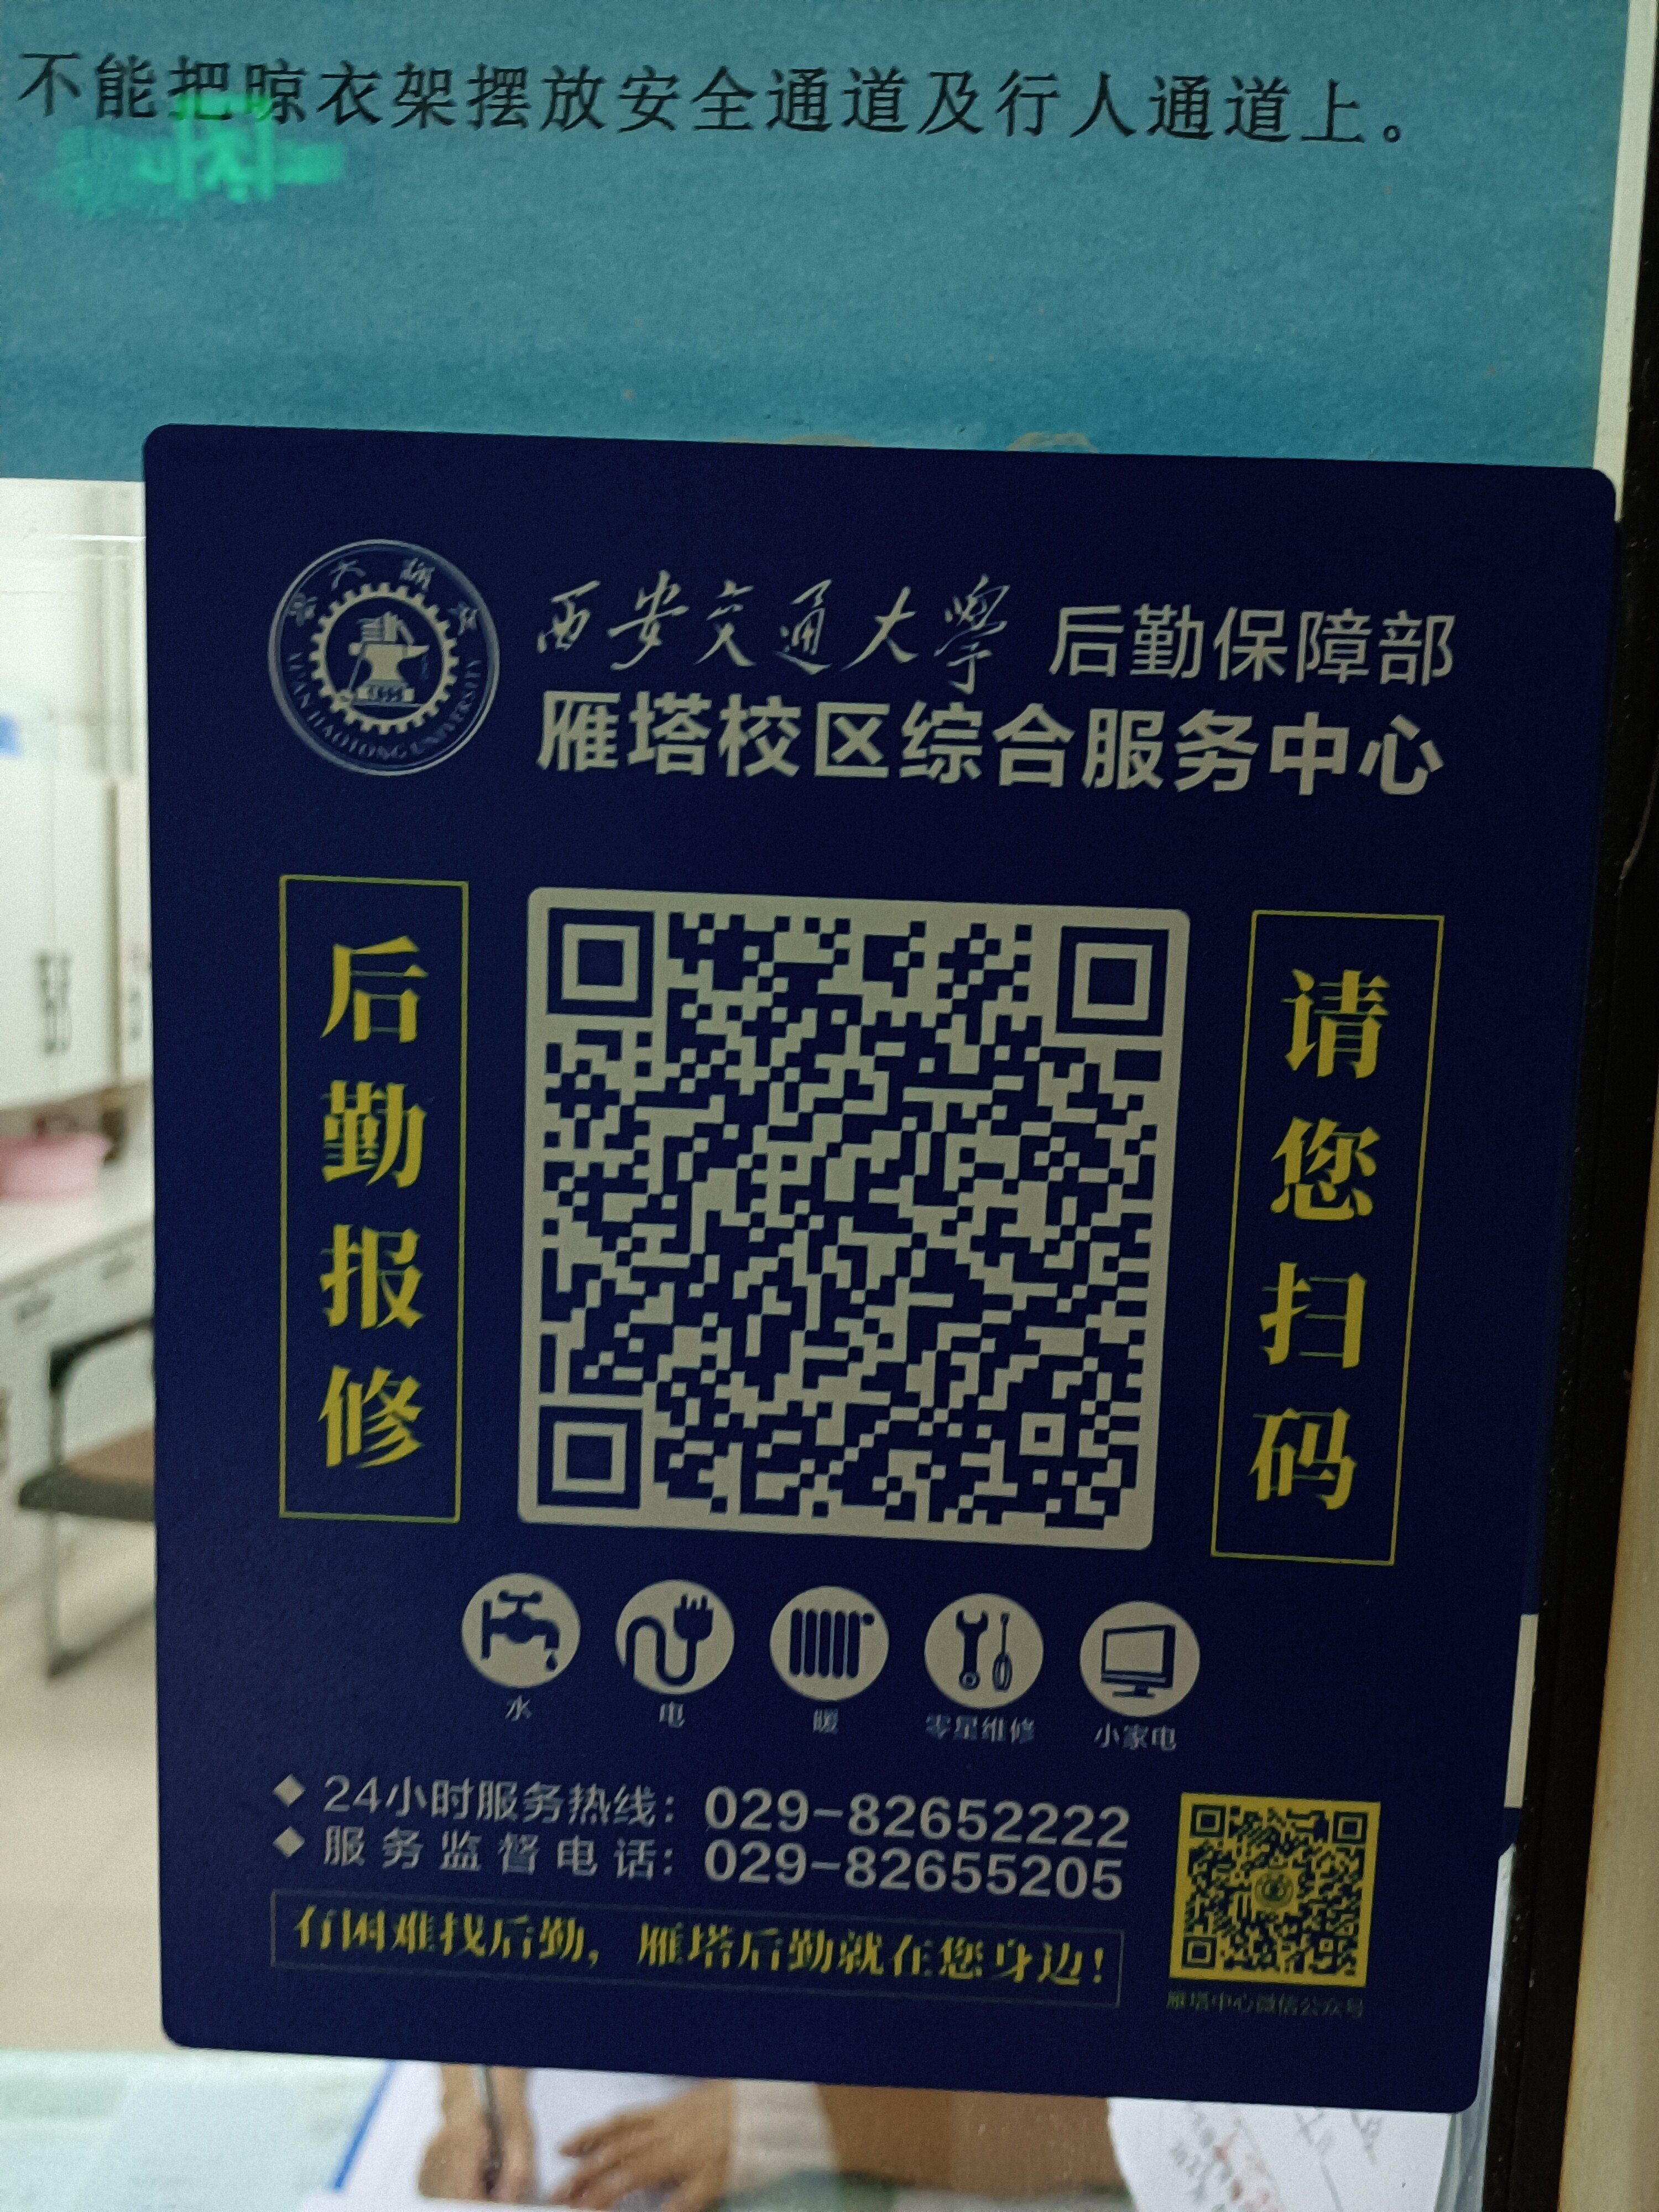
\includegraphics[width=1\linewidth]{media/image6.jpg}
    \caption{后勤报修二维码}
    \label{fig:QR}
\end{figure}


\textbf{据说今年好多高校可以自选宿舍和床位,还可以发“简历”招舍友,狠狠羡慕辽d({\H{O}}д{\H{O}}๑)}
\section{实习科室攻略}

\subsection{总体}


\begin{itemize}
\item 实习开始时间是五月底,有一周的院前培训,比较水。
\item 每三周轮转一个科室,每个科基本都有教学查房和小讲课,需要签到考勤,查的不是很严,出科六份大病历是标配,一般有出科考试,比较简单。
\item 实习部分科室只需跟随早上查房,值班一次或两次即可,部分科室比较严格,建议及时和上一轮科室同学打听,以免影响出科。
\item 实习取决于自己,考研保研还是实习哪个更重要,相信大家有自己的选择。
\end{itemize}
\subsection{各个科室}

\begin{itemize}
\item 精神:挺好
\item 社区:挺好,建议不要去儿保和检查
\item 急诊:嗯就老老实实去上班吧  
\item 产科:挺好
\item 妇科:挺好,但最好不要去wj组
\item 泌外:挺好,带教没什么事但cjq住院总可能查人,sb
\item 骨科:很好,带教不太管,住院总lt很幽默
\item 肝胆:四个病区各有千秋,一病区带检查较多,二病区胰腺病)大瓜PC+性别歧视),三病区肝移植,四病区肝外科糖尿病相关(住院总ybw在四病区,他其实还比较好说话)
\item 儿科:如果sf不当住院总,好炸了,老师们教学很认真,推荐血液组,想事少去神经,不推荐肾病组, 如果值班遇到sf,别理sb,自己去写交班本
\item 心内:老师人很好,可以水也可以学到很多东西,平价一天拉四五个心电图,跟老师搞好关系说不定可以去介入室看看。门诊值班量一天血压(水银的!),提前做好心理准备。
\item 感染:早交班部分老师会让现场签到,建议去。教学活动会经常临时换时间后推。跟查房时建议主动提手消,彰显存在感。
\item 内分泌:值班需要早5晚9查血糖(随年份不同可能有变动,现在早5已经取消了。)老师在查房时会讲知识点,想学是可以学到很多东西,可以提手消增加存在感,但需要把握挤手消的时间节点。交班手写,每个新病人和危重都要详细交,很可能要写2h左右。
\item 神内:非常水,老师基本不管,交班为电子版打印,内容较少。周内固定几天大交班不需要实习生念。假期值班也轻松,早上不用去交。但病历很长,不推荐攒到最后。
\item 呼内:比较水。因科室规模较大,不同组别不同分区可能有差异,推荐A区。需要排班去带病人做检查,带检查时下班时间不固定。
\item 儿科门诊:挺好,不排班就是假。
\end{itemize}
\chapter{校外生活}
大学生活从来都不仅仅在大学,探索这座城市,发掘爱好事物更是大学的一部分。无论你爱好自然,还是偏爱城市,喜欢独处,还是呼朋唤友,希望以下活动都能为你提供一些参考。

\section{一般活动}

电影,KTV,剧本杀,密室逃脱等等。以上不做推荐,根据个人需求,小寨有很多,可自行选择。

\section{交通方式}

\subsection{地铁}

纬一街站 (2号线) 、小寨 (2或3三线) 、古祥州站 (3号线)

特别提醒: 小寨站在旅游高峰期 (暑寒假及节假日) 时较为拥挤

\subsection{公交}
\begin{itemize}
    \item 交大一附院公交站: 5路、18路/K18路、19路、30路/K30路、106路、136路、146路、156路、196路。

    \item 西八里村公交站: 5路、18路/K18路、30路/K30路、106路、146路、196路、203路229路。

    \item 长安路雁塔西路公交站: 5路、12路、19路、136路、146路、156路、196路、215路/K215路、285路、401路。
\end{itemize}
\subsection{校区间通勤方式}
\begin{itemize}
    \item 雁塔校区一兴庆校区

校车: 20\textasciitilde{}30分钟

地铁: 6号线转2号线,30分钟

骑行: 35分钟

\item 雁塔校区一创新港:

校车: 55分钟

地铁: 2号线转5号线,90分钟
\end{itemize}


\section{书店}
\begin{itemize}
\item 嘉汇汉唐书城
\item 新华书店(小寨书店)
\item 西西弗书店(momopark店)
\item 曲江书城-新华书店
\item 茑屋书店
\end{itemize}
以上书店环境及其地理位置都很好,可以随意选择一个午后静静享受阅读的一天。

\section{展览}

不如去看展吧!既可以消磨时光又享受到了好看的展览,可以独自一人,也可以和朋友一起,谁能不喜欢看展呢?
获取最近展览信息可以关注以下相关公众号:
\begin{itemize}
\item 陕西历史博物馆:需要提前预约
\item 西安美术馆:需要提前预约
\item 陕西省美术博物馆:无需预约
\item 西安市城市影像博物馆(大都荟):无需预约
\item 西安博物院:需要提前预约
\item 陕西考古博物馆:需要提前预约(位置比较远,建议留出一整个白天,附近有香积寺古刹(非小红书上斋饭很好吃、手串很出圈的那个杭州香积寺),但是风景也很好,和网红打卡地古寺的氛围截然不同,寺院外有很多小商贩,市井气十足。
\end{itemize}
以上均为免费展览,其余展览信息可在某书实时搜索西安展览获取。

\section{美食}

西安作为碳水之都,有很多很多平价又好吃的美食,任何时间任何地点你都可以找到你爱的那一碗西安美食。美食的力量是无穷的,来自一个热爱美食人的呐喊{\fontspec{Symbola}\char"1F4AA}。

\subsection{推荐西安本地博主}


\begin{itemize}
\item 君在西安 这位up很能吃辣,饭量也很厉害,爱吃辣的朋友可以关注君。
\item 可爱的鹅儿er 推荐这位up,很可爱!而且去了好几次推荐的美食,都很喜欢。
\end{itemize}
本人实际都去过两位up推荐的店,好吃的。可以随意选择视频里感兴趣的餐厅,一般情况下不会踩雷。

\subsection{推荐学校附近美食聚集地}


\begin{itemize}
\item 红砖南路:小店很多,有早市也有适合夜市的烧烤、火锅、打边炉之类,一人食或多人均可。
\item 翠华路:陕历博旁边的腊汁肉揪面片,各种面,都好吃
\item 夏家庄:公交夏家庄站旁边的一条街,满满都是不同的店:面皮,各种面,自助火锅,东北菜,潮汕大排档……美的很{\fontspec{Symbola}\char"1F60D}
\end{itemize}

并不推荐商场内美食,一般人均都会70左右且口味一般,推荐性价比更高且味道更好的街边小店,西安的面不需要去网红店,随便找个距离最近的小店都会很好吃。

当然以上地方的店我没有一一尝试,去过其中一部分都还不错,所以列在里面。除了以上,也可以使用某点评软件接收美食安利,但需认真鉴别,祝大家都能在西安吃的幸福{\fontspec{Symbola}\char"1F606}。

\subsection{喝点什么}


\begin{itemize}
\item 各大著名奶茶品牌就不在此赘述了,每人口味不同,且不宜常喝不做推荐。虽然我常喝{\ldots} {\ldots}之所以提一下呢,是每每期末月时,都会点奶茶陪我度过难易度过的期末月,如果难过喝点甜的,就继续生活吧。
\item 各种茶包 正在测评中,茶颜茶包还可以,但略贵,可以尝试。此部分待完善。
\item 自制水果汁:健康又美味,购入微型榨汁杯,放入西瓜,倒入冰块(一元可在学校益禾堂购入,永远怀念离开的益禾堂),一杯非常适合夏天的冰镇西瓜汁就制作完成了。一根香蕉,一袋放在暖气片上的热牛奶,可加些燕麦,一杯非常适合冬天的香蕉燕麦牛奶就好了。
\item 咖啡:希望那俩家咖啡品牌永远8.8,9.9,就近就可选择这两个品牌,除此可购入咖啡液或其他,blendy性价比不错,本人非咖啡爱好者,只是为了防困,如果有同学愿意完善这一部分,请联系我的邮箱。(追求口感可以用速溶黑咖啡加鲜牛奶加东方树叶)
\end{itemize}
\section{脱口秀}
\begin{itemize}
\item 可乐喜剧:分为商演和开放麦,开放麦很便宜6.6元,当然质量无法保证,大多都是在打磨阶段,商演价格一百左右,内容就会好很多,可以都体验一下。 位于大悦城。
\item 唐蒜铺子 好评还可以,但本人没去过
\end{itemize}
\section{演出}
\begin{itemize}
\item 可以关注陕西大剧院x西安音乐厅的公众号与某宝店铺,经常会有80\textasciitilde{}100元的学生票与公益票,还是值得一看的。
\item 除了陕西大剧院,靠近北大街还有五四剧院和人民大剧院等剧院,还有青曲社等会进行很多相声演出。
\item 可以关注陕西文旅惠民公众号,经常会有演出的优惠票,可以便宜几十块钱。节假日还有200块钱的惠民卡,需要抢。
\end{itemize}
\section{足浴}
金色印象、泽西岛、水木和,小贵但身心都很放松。
\section{KTV}

学校附近有:音乐汇量贩KTV(可以调key,很8错)、魅KTV、魔方KTV、星聚会KTV、唱吧麦颂KTV(这些都是学校附近比较便宜的,非热门时间段小包基本不过百,魅可能略贵一丢丢)同学聚会,生日party,失恋放纵,考试月胜利结算、失败总结等,都很适合,属于大俗大雅。期待解锁更多KTV场合。

\section{户外体能活动}
\begin{itemize}
\item 爬山:
\begin{enumerate}
\item 翠华山:距离西安市区最近的山,可以公交车直达,适合新手
\item 华山:属于著名景点,人会很多,可以当做短途旅行
\item 终南山:秦岭最高峰,难度较大,部分人会出现高反
\item 骊山:位于临潼区,包含著名景点华清池(其实是演出比较出名),景区内不算太高,景区外有一条环山公路常有摩托聚会(真的很多摩托,超酷),聚会点为藤原豆腐店,适合打卡拍照
\item 南五台山:不算太高,适合新手,山顶风景很好,建议雨后多云去,说不定有云海。
\item 牛背梁:景区很大,难度适中,可以当做短途旅行
\item 太白山:著名景点需要提前预约,但风景秀丽周围还有温泉,缺点是有些远
\item 秦岭72峪口,朱雀森林公园,黑河森林公园都是秀美山水便不一一赘述,进山,是刻在每个西安人DNA里的\textasciitilde{}
\end{enumerate}

\item 划船:最直接的方式其实是加入赛艇俱乐部去咱们学校自己的赛艇基地hhh,其余都是景区里那种,较为休闲娱乐的,不做赘述
\item 放风筝:基本每年学校都会举办放风筝活动(宗濂书院宿安会),场地为学校操场,除此之外,西安春季(2-4月)的时候,在市区各种公园及杜陵塬、乐游原、渭河运动公园等地势平坦处都会有许多人放风筝,风筝样式也很多,大家可以自行挑选。
\item 滑雪:冬季西安周边有许多雪场,翠华山、竹林畔、更远的有鳌山,学校的轮滑俱乐部也会组织大学生滑雪活动,详情自行咨询。
\item 徒步穿越:西安山多驴友也很多,会有比较专业的团队组织徒步穿越,喜欢户外活动的小伙伴可以自行探索(本人参与过西安深呼吸户外俱乐部的活动,仅供参考)
\item 户外露营:据说露营的黄金期已经过去了,但周末租个帐篷去露营烧烤还是很快乐的,可以带上趁手的乐器,带本书,下午看书喝茶晒太阳,晚上篝火吉他看星空,又能勇敢面对下一周的狗x生活了!
\end{itemize}
\section{室内体能活动}
在此不做具体推荐,只是开拓大家娱乐的多面性
\begin{itemize}
\item 攀岩
\item 蹦床
\item 轮滑、滑冰、滑雪(目前西安新开一家规模较大室内雪场,感兴趣可前去体验)
\item 射箭
\item VR
\item 卡丁车
\end{itemize}
\section{二次元}

作为阳光的二次元当然要走出宿舍多多活动,\sout{不能当阴暗宅宅}

\subsection{漫展}
\begin{itemize}
\item 学校本身会举办樱花动漫节(当然在东区),很多同学都会出cos
\item 可以在B站会员购搜索西安举办的漫展 ,浅浅避雷一下大华这个场地,很远且破旧
\item 西安的联动活动还是比较多的(当然不比上海成都),基本会在商场或是餐厅进行,商场一般就是游戏直播,随机舞蹈,嘉宾签售等等,餐厅参考原神。
\end{itemize}
\subsection{吃谷(goods,周边)}

2023年可以说是西安谷圈元年,西安的谷店如雨后春笋一般四处开花,本人将持续更新探店
\begin{itemize}
\item 西谷万事屋:位于中贸广场,店面中等,日谷居多,有寄售,价格较合理
\item 谷咩:位于老菜场(城墙里,原来是菜市场现在改造成创意街区了,还有不少中古店),店面偏小,国谷较多,价偏高
\item 方所:其实是老城根的一家书店,有2层,IP较多但比较分散,基本为大热IP(有明日方舟稀有谷),不为买谷也是值得一去的书店
\item 民乐园2家
\item 龙首原1家
\item 各处商场的潮玩文创店也会有少量原神及热门bl作品的谷,这种就随缘吧
\end{itemize}
\subsection{三坑}

学校早前也有三坑交流群,不过好像已经沉寂很久(详情自行咨询学姐)
\begin{itemize}
\item 汉服:汉服就不赘述了,西安满街头都是汉服妆造,目前是汉服的天下
\item Lolita:实体店经历过一批倒闭潮,目前比较稳定的有赛格B2仲夏物语,海港城B2七岁半,老城根Gpark Daydream
\item JK:\sout{2023年还有人穿jk吗55555,}西安的线下店都不进行推荐,审美不算太好
\end{itemize}

\textbf{当然有条件的情况下推荐乘坐3小时高铁前往成都,那里才是阴暗宅宅的快乐老家\textasciitilde{}}
\chapter{如何保持身心健康}
\section{碎碎念}

其实这一部分是整个文档我最想写,认为最重要的部分,因为在这里我并没有身心健康,我知道处于非健康状态是怎样的,写下这些是希望更多的人能够尽量保持身心健康。

\section{身体健康}

不熬夜,饮食健康,适度运动,做好清洁卫生,其实谁都知道保持健康的重要性,也知道如何保持健康,只是每一点都做到似乎对于大学生很难,我也没有做到,只能说尽力改善调整自己的状态。去跑步,去流汗真的很快乐,几周没有喝奶茶也不是难做到的事情,重要的是去踏出第一步,去尝试总比停在原地好。

\section{心理健康}
\begin{itemize}
\item 其实每个人的心理健康程度不尽相同,每个人都是独特的,我只能讲我如何调节自身的,希望能做到抛砖引玉的作用吧。
\item 心理健康非常非常重要,如果发现自己有情绪不佳的状态,一定一定多加注意,不要一直放任其发展,我也曾经认为我不会发生心理健康问题,但它就是发生了,没有人能够信誓旦旦地保证未来,所以自己多加注意很重要。
\item 找寻原因,是为什么呢,是怎么一步一步到现在的,我这样问过自己,环境因素,学业因素,无法获得正反馈,无法从外部获得能量等等。
\item 如何改善,知道了原因,那接下来能做些什么呢,分步解决。环境因素对于我其实无法改善,根本解决方法\textemdash{}\textemdash{}毕业迅速离开toxic的医学部。学业因素,无法真正喜欢临床医学,那就换个方向探索,拿不到高gpa我就一事无成了吗,探索其他方向的实验项目,做学生活动,参与公益组织,读更多的闲书,花费更多时间用英语交流探索,探索这座城市的美食,我做了上述很多可能无用但让我感到充实有趣的事情,我知道我在慢慢走出,虽然没有完全但有在变好,我不知道恢复的时间需要多久,我只能讲只有去尝试,去探索才有变好的可能性。
\item 寻求帮助,其实我个人认为这是很难的部分,在我未曾陷入心理非健康状态时,也会冠冕堂皇得讲说出来就好了,应该及时寻求专业医生咨询,但不是这样的,很多时候很容易深陷情绪之中,很难去寻求帮助,只有在变好之后我才有勇气讲其实过去一年多我过得非常不好,真正帮助我的其实是我自己,但如果你真的很长时间情绪不佳,程度很深,请一定一定去寻求专业帮助,只是我是一直相信自己可以恢复,世界有很多美景,为什么要因为一时的环境而深陷其中,总有结束的时候,广阔天地,希望我们有勇气去探索。
\item 找到自己喜欢的方向,其实这点很难很难做到。我们一直在做题中度过,拿到好成绩似乎是唯一的评价标准,但生活不是这样的,除了gpa之外我到底喜欢什么是我认为我们每一个人都应该在大学思考的问题。怎么找到喜欢的方向,这个问题其实我也没有办法回答,只有多多尝试才有机会找寻到,比如我组织参与了很多社团活动才发现我其实是喜欢与人沟通交流的过程,比如我看了很多美剧或在英文网络闲逛,和国外的人交流后才发现我好像对英语已经会基本日常应用了,即使我并没有认真去学习去做题,比如我接触了编程之后,才发现我其实很喜欢能够通过编程可以让自己的想法变成实际的一个过程,能有一定创造性的工作或许很适合我,包括做一些人格测试,也可以发现像我enfp可能更适合做咨询和教育相关领域,那就可以多在这样的领域探索,每个人喜欢擅长的领域不同,这里推荐两本书,可以进行阅读更加了解自己,包括里面有一些方法个人觉得比较实用,可以实际应用一下。《斯坦福大学人生设计课》和《天生不同》,当然这只是我的个人经历,比较局限,希望这部分能有更多同学分享,如果可以请联系我。
\item 请多夸夸自己,也请毫不吝啬地多夸夸别人。其实这点也很重要,多给自己积极的心理暗示,而且不一定要是很厉害的事,比如我很会找好吃的地方,今天发现了一个新外卖很好吃,推荐给了同学大家都觉得不错,那说明我很会观察,很会挑选,很会安利,这很厉害啊,就很小的事情但同样值得夸赞。当然也多多夸赞他人,给予别人积极的外部反馈,其实我们每个人都有很多很多闪光点,只是很多时候因为评价体系的关系,我们自己都会忽略掉自己是很优秀的很棒的人,所以不用陷入学校单一的评价体系,找到自己合适的,去发展自己的长处吧\textasciitilde{}{\fontspec{Symbola}\char"1F44F}{\fontspec{Symbola}\char"1F60D}
\end{itemize}
\chapter{特别篇(3):雁塔校区的猫猫}
\begin{example}
    本篇由“学校东边第一个垃圾桶”编写,VX13309271992
\end{example}
\begin{theorem}
    请大家爱护猫猫,严禁伤害猫猫!!!
\end{theorem}
\section{宗濂大院}
在生活区,往里走右边的大院里,通常嘬嘬嘬一下毛米们就屁颠屁颠来讨饭了,随运气遇见,靠近不跑的可上手撸\textasciitilde{}
\begin{enumerate}
    \item \hyperref[img12]{黑漆漆}:抹布2022秋的孩子,黑压压的姐妹
    \begin{figure}[htbp]
            \centering
            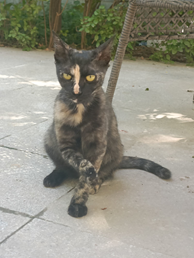
\includegraphics[width=0.4\linewidth]{media/cimage1.png}
        \qquad
            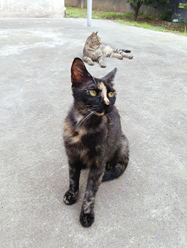
\includegraphics[width=0.4\linewidth]{media/cimage2.png}
            \caption{黑漆漆}
            \label{img12}
    \end{figure}
    \item \hyperref[img34]{黑压压}:抹布2022的孩子,黑漆漆的姐妹
    \begin{figure}[htbp]
            \centering
            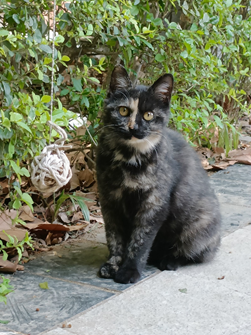
\includegraphics[width=0.4\linewidth]{media/cimage3.png}
        \qquad
            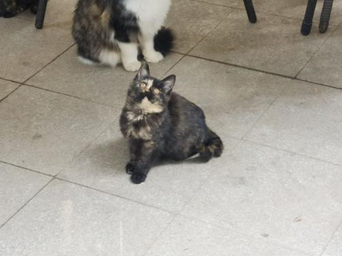
\includegraphics[width=0.4\linewidth]{media/cimage4.png}
            \caption{黑压压}
            \label{img34}
    \end{figure}
        \item \hyperref[img56]{百里}:蒲公英的孩子
    \begin{figure}[htbp]
            \centering
            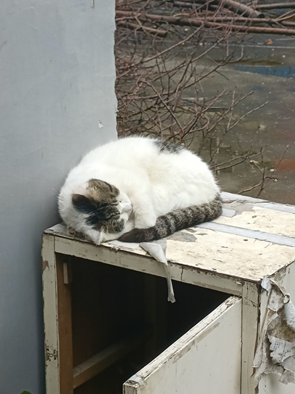
\includegraphics[width=0.4\linewidth]{media/cimage5.png}
        \qquad
            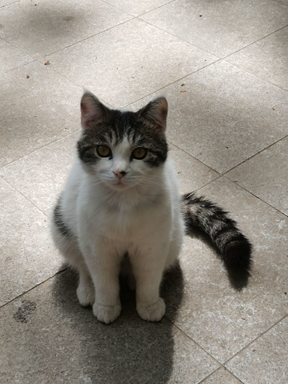
\includegraphics[width=0.4\linewidth]{media/cimage6.png}
            \caption{百里}
            \label{img56}
    \end{figure}
        \item \hyperref[img78]{大呆}:烦烦和横眉的孩子
    \begin{figure}[htbp]
            \centering
            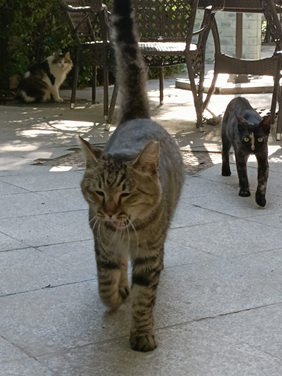
\includegraphics[width=0.4\linewidth]{media/cimage7.png}
        \qquad
            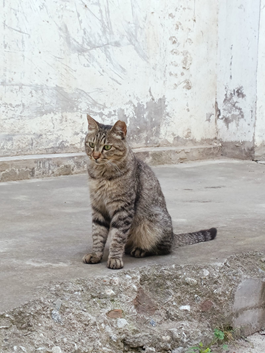
\includegraphics[width=0.4\linewidth]{media/cimage8.png}
            \caption{大呆}
            \label{img78}
    \end{figure}
        \item \hyperref[img910]{小呆}:蒲公英2023之子
    \begin{figure}[htbp]
            \centering
            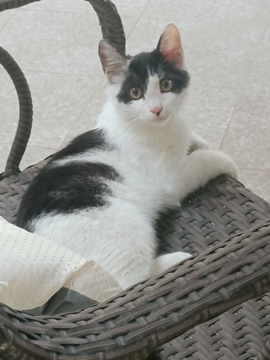
\includegraphics[width=0.4\linewidth]{media/cimage9.png}
        \qquad
            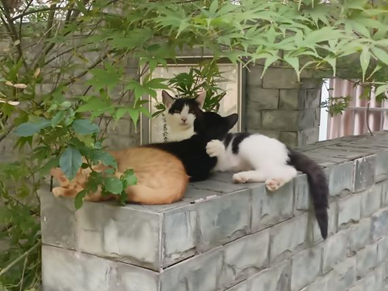
\includegraphics[width=0.4\linewidth]{media/cimage10.png}
            \caption{小呆}
            \label{img910}
    \end{figure}
        \item \hyperref[img111213]{蒲公英}:烦烦和横眉的孩子
    \begin{figure}[htbp]
            \centering
            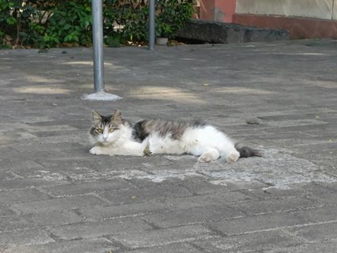
\includegraphics[width=0.4\linewidth]{media/cimage11.png}
        \qquad
            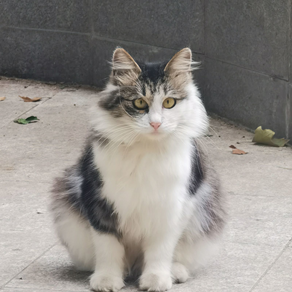
\includegraphics[width=0.4\linewidth]{media/cimage12.png}\\
            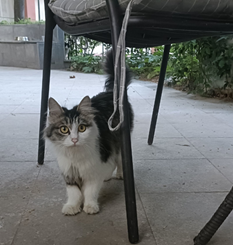
\includegraphics[width=0.4\linewidth]{media/cimage13.png}
            \caption{蒲公英}
            \label{img111213}
    \end{figure}
        \item \hyperref[img141516]{吐司与可可}:漆漆之子,生于2023.5.13
    \begin{figure}[htbp]
            \centering
            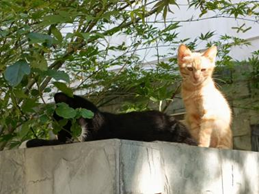
\includegraphics[width=0.4\linewidth]{media/cimage14.png}
        \qquad
            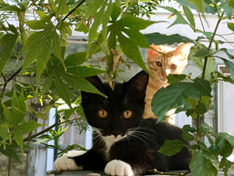
\includegraphics[width=0.4\linewidth]{media/cimage15.png}\\
            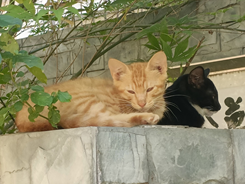
\includegraphics[width=0.4\linewidth]{media/cimage16.png}
            \caption{吐司与可可}
            \label{img141516}
    \end{figure}
        \item \hyperref[img17]{小花}:嗯......见得较少
    \begin{figure}[htbp]
            \centering
            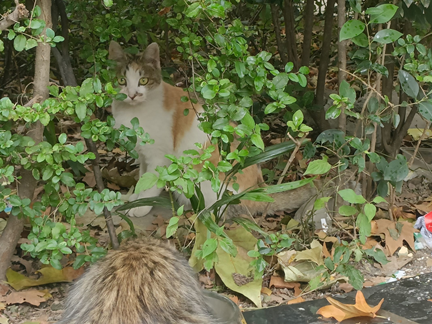
\includegraphics[width=0.4\linewidth]{media/cimage17.png}
            \caption{小花}
            \label{img17}
    \end{figure}
        \item \hyperref[img1819]{抹布}:老狸\&横眉之女,小咪、黑漆漆黑压压之母
    \begin{figure}[htbp]
            \centering
            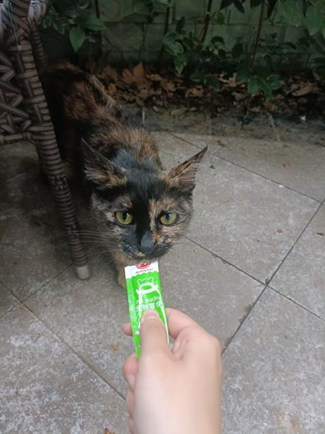
\includegraphics[width=0.4\linewidth]{media/cimage18.png}
        \qquad
            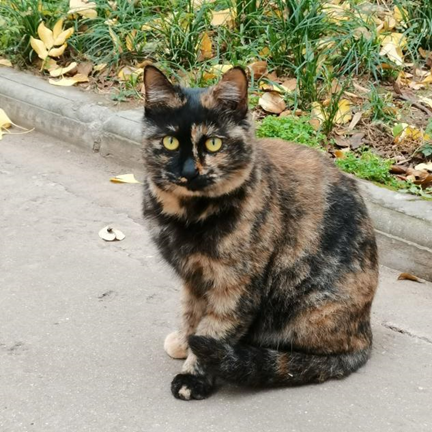
\includegraphics[width=0.4\linewidth]{media/cimage19.png}
            \caption{抹布}
            \label{img1819}
    \end{figure}
        \item \hyperref[img2021]{李白}:蒲公英的孩子
    \begin{figure}[htbp]
            \centering
            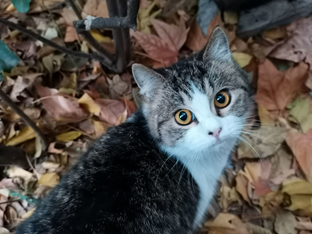
\includegraphics[width=0.4\linewidth]{media/cimage20.png}
        \qquad
            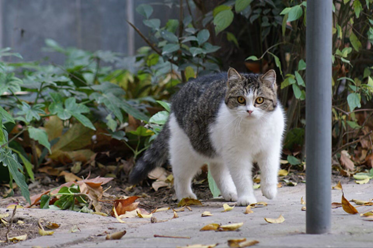
\includegraphics[width=0.4\linewidth]{media/cimage21.png}
            \caption{李白}
            \label{img2021}
    \end{figure}
        \item \hyperref[img2223]{黑背}:生了病的可怜宝宝QAQ
    \begin{figure}[htbp]
            \centering
            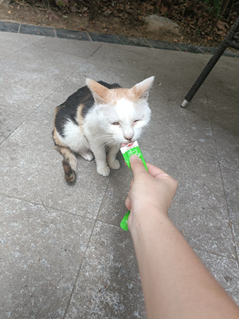
\includegraphics[width=0.4\linewidth]{media/cimage22.png}
        \qquad
            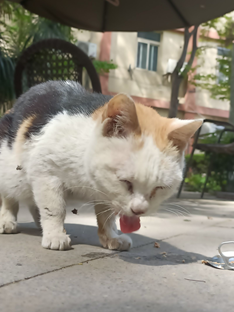
\includegraphics[width=0.4\linewidth]{media/cimage23.png}
            \caption{黑背}
            \label{img2223}
    \end{figure}
        \item \hyperref[img2425]{横眉}:院里大种公,聪明过人,已噶
    \begin{figure}[htbp]
            \centering
            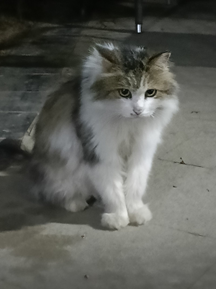
\includegraphics[width=0.4\linewidth]{media/cimage24.png}
        \qquad
            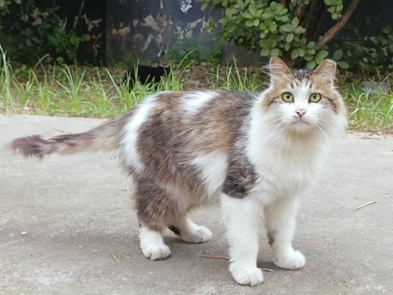
\includegraphics[width=0.4\linewidth]{media/cimage25.png}
            \caption{横眉}
            \label{img2425}
    \end{figure}
            \item \hyperref[img2627]{墨翠}:烦烦和横眉的孩子
    \begin{figure}[htbp]
            \centering
            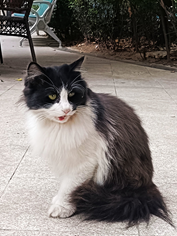
\includegraphics[width=0.4\linewidth]{media/cimage26.png}
        \qquad
            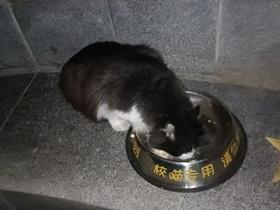
\includegraphics[width=0.4\linewidth]{media/cimage27.png}
            \caption{墨翠}
            \label{img2627}
    \end{figure}
\end{enumerate}
\section{财主}
在楼里或者楼附近刷新。
\begin{enumerate}
    \item \hyperref[img2829]{闹闹}:通常游荡在财主楼内,在二楼教室里随机刷新,头可以随便摸,有时候会出去拉屎
    \begin{figure}[htbp]
            \centering
            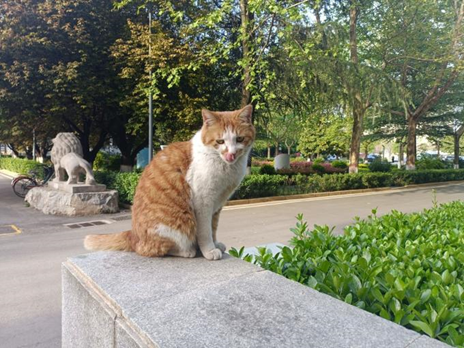
\includegraphics[width=0.4\linewidth]{media/cimage28.png}
        \qquad
            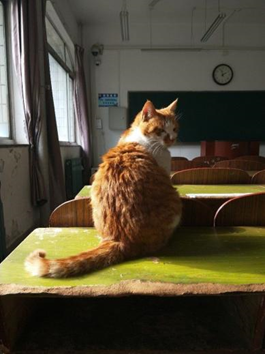
\includegraphics[width=0.4\linewidth]{media/cimage29.png}
            \caption{闹闹}
            \label{img2829}
    \end{figure}
    \item \hyperref[img3031]{庞丽丽(胖狸狸的谐音)}:财主后面游荡,特别亲人,手感嘎嘎好,随便摸
    \begin{figure}[htbp]
            \centering
            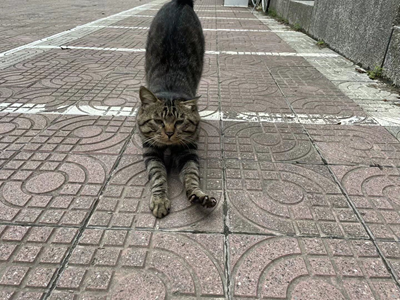
\includegraphics[width=0.4\linewidth]{media/cimage30.png}
        \qquad
            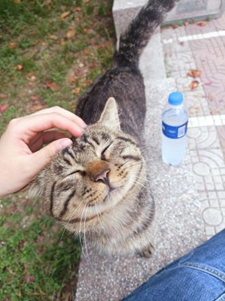
\includegraphics[width=0.4\linewidth]{media/cimage31.png}
            \caption{庞丽丽(胖狸狸的谐音)}
            \label{img3031}
    \end{figure}
        \item \hyperref[img3233]{咪咪}:本来是性感猫妈,绝育后变火辣大地雷
    \begin{figure}[htbp]
            \centering
            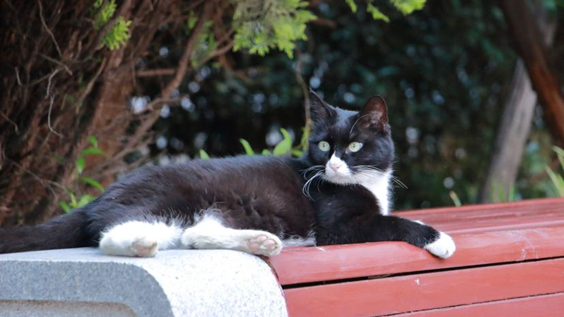
\includegraphics[width=0.4\linewidth]{media/cimage32.png}
        \qquad
            
\includegraphics[width=0.4\linewidth]{media/cimage33.png}
            \caption{咪咪}
            \label{img3233}
    \end{figure}
        \item \hyperref[img3435]{虎纹}:乖乖小美女
    \begin{figure}[htbp]
            \centering
            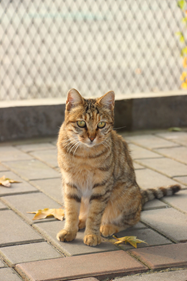
\includegraphics[width=0.4\linewidth]{media/cimage34.png}
        \qquad
            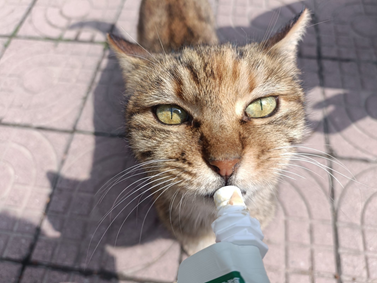
\includegraphics[width=0.4\linewidth]{media/cimage35.png}
            \caption{虎纹}
            \label{img3435}
    \end{figure}
    \end{enumerate}
\section{病理楼}
\begin{enumerate}
    \item \hyperref[img3637]{罗恩}:一只见了生人就跑的很快的小毛米
    \begin{figure}[htbp]
            \centering
            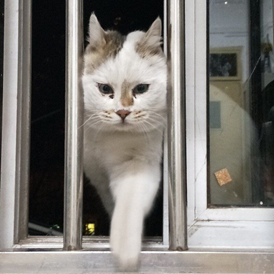
\includegraphics[width=0.4\linewidth]{media/cimage36.png}
        \qquad
            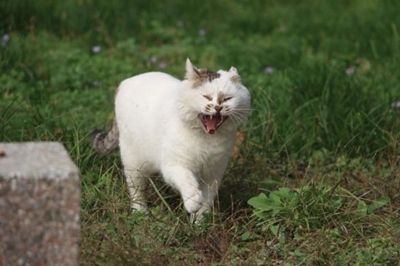
\includegraphics[width=0.4\linewidth]{media/cimage37.png}
            \caption{罗恩}
            \label{img3637}
    \end{figure}
    \end{enumerate}
\section{启德花园}
\begin{enumerate}
    \item \hyperref[img38]{蜡笔}:sunshine2023夏的孩子
    \begin{figure}[htbp]
            \centering
            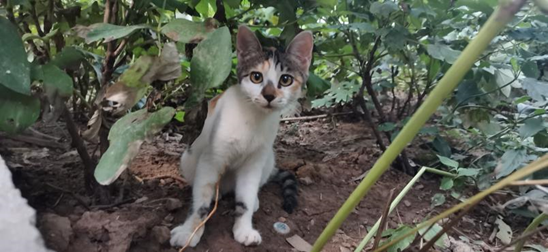
\includegraphics[width=0.4\linewidth]{media/cimage38.png}
            \caption{蜡笔}
            \label{img38}
    \end{figure}
    \item \hyperref[img3940]{大白}:乖乖白
    \begin{figure}[htbp]
            \centering
            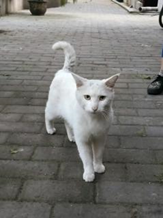
\includegraphics[width=0.4\linewidth]{media/cimage39.png}
        \qquad
            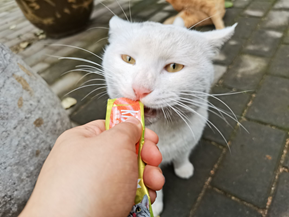
\includegraphics[width=0.4\linewidth]{media/cimage40.png}
            \caption{大白}
            \label{img3940}
    \end{figure}
        \item \hyperref[img4142]{sunshine}:面包、招财金宝、蜡笔的妈咪,暖黄色小毛米,西区颜值巅峰
    \begin{figure}[htbp]
            \centering
            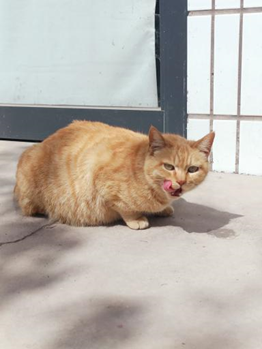
\includegraphics[width=0.4\linewidth]{media/cimage41.png}
        \qquad
            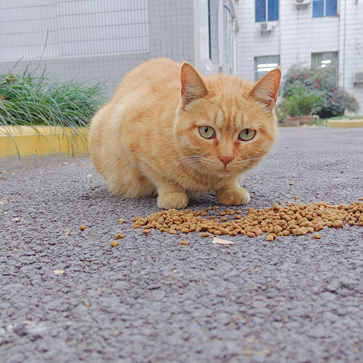
\includegraphics[width=0.4\linewidth]{media/cimage42.png}
            \caption{sunshine}
            \label{img4142}
    \end{figure}
    \end{enumerate}
\section{解剖楼}
\begin{enumerate}
    \item \hyperref[img4344]{面包}:sunshine的孩子,有口炎的可怜宝宝
    \begin{figure}[htbp]
            \centering
            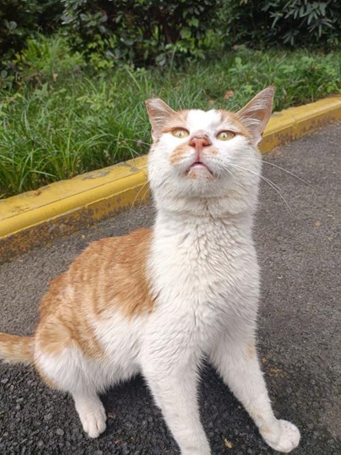
\includegraphics[width=0.4\linewidth]{media/cimage43.png}
        \qquad
            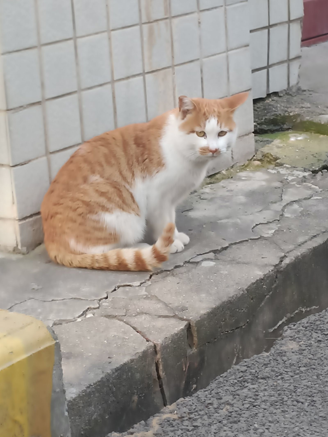
\includegraphics[width=0.4\linewidth]{media/cimage44.png}
            \caption{面包}
            \label{img4344}
    \end{figure}
        \item \hyperref[img4546]{招财\&金宝}:sunshine和大白2022的孩子,背上橘色多的是金宝,背上橘色少的是招财,招财23.3.21已逝
    \begin{figure}[htbp]
            \centering
            \includegraphics[width=0.4\linewidth]{media/cimage45.png}
        \qquad
            \includegraphics[width=0.4\linewidth]{media/cimage46.png}
            \caption{招财\&金宝}
            \label{img4546}
    \end{figure}
    \end{enumerate}
\section{停车场}
\begin{enumerate}
    \item \hyperref[img47]{MI家族·梅川酷仔}:蝴蝶结2023夏的孩子,梅MILY川MIVI酷MIKO仔MIU。梅梅是三花 ,川川是橘白,酷酷是全橘,仔仔是奶牛
    \begin{figure}[htbp]
            \centering
            \includegraphics[width=0.4\linewidth]{media/cimage47.png}
            \caption{MI家族·梅川酷仔}
            \label{img47}
    \end{figure}
    \end{enumerate}
\section{药学楼}
\begin{enumerate}
    \item \hyperref[img48]{点点鼻}:见到的较少
    \begin{figure}[htbp]
            \centering
            \includegraphics[width=0.4\linewidth]{media/cimage48.png}
            \caption{点点鼻}
            \label{img48}
    \end{figure}
        \item \hyperref[img4950]{刀哥}:小眼屎小三花的爸爸
    \begin{figure}[htbp]
            \centering
            \includegraphics[width=0.4\linewidth]{media/cimage49.png}
        \qquad
            \includegraphics[width=0.4\linewidth]{media/cimage50.png}
            \caption{刀哥}
            \label{img4950}
    \end{figure}
    \end{enumerate}
\section{西花园}
\begin{enumerate}
    \item \hyperref[img5152]{委屈屈}
    \begin{figure}[htbp]
            \centering
            \includegraphics[width=0.4\linewidth]{media/cimage51.png}
        \qquad
            \includegraphics[width=0.4\linewidth]{media/cimage52.png}
            \caption{委屈屈}
            \label{img5152}
    \end{figure}
        \item \hyperref[img5354]{小馒头}
    \begin{figure}[htbp]
            \centering
            \includegraphics[width=0.4\linewidth]{media/cimage53.png}
        \qquad
            \includegraphics[width=0.4\linewidth]{media/cimage54.png}
            \caption{小馒头}
            \label{img5354}
    \end{figure}
            \item \hyperref[img5556]{冷漠}:冷漠不冷,只是怂
    \begin{figure}[htbp]
            \centering
            \includegraphics[width=0.4\linewidth]{media/cimage55.png}
        \qquad
            \includegraphics[width=0.4\linewidth]{media/cimage56.png}
            \caption{冷漠}
            \label{img5556}
    \end{figure}
    \end{enumerate}
\section{护理楼}
\begin{enumerate}
    \item \hyperref[img5758]{乐乐}:橘头小猫,经常受欺负但又很坚强,可以叫它``不苦''
    \begin{figure}[htbp]
            \centering
            \includegraphics[width=0.4\linewidth]{media/cimage57.png}
        \qquad
            \includegraphics[width=0.4\linewidth]{media/cimage58.png}
            \caption{乐乐}
            \label{img5758}
    \end{figure}
    \end{enumerate}
\section{卫法楼}
\begin{enumerate}
    \item \hyperref[img5960]{扒窗台}
    \begin{figure}[htbp]
            \centering
            \includegraphics[width=0.4\linewidth]{media/cimage59.png}
        \qquad
            \includegraphics[width=0.4\linewidth]{media/cimage60.png}
            \caption{扒窗台}
            \label{img5960}
    \end{figure}
    \end{enumerate}
    
\chapter{特别篇(4):XJTU基础医学生存指南}

\section{说在前面的话}

去年这个时候,我一想到我的本科要读五年这件事就无比懊恼\textemdash{}\textemdash{}我的朋友们多数四年制正准备美美地步入人生的下一个阶段但我还要多读一年,拿着一个所谓的医学学位却只能干生物的活。但事实上,本科五年也是说过去就过去了,关于曾经无忧无虑的日子的记忆已经逐渐模糊,我似乎已经变成了一个二十多岁前途迷茫的废物。

从高考结束到进入西交,再到现在刚刚画完一个逗号,我经历过欣喜若狂,也经历过自我怀疑,我想过窝在舒适圈,也尝试过雷区......我当然还有很多欠缺,但这两年的经历也不只是让我徒增岁月。

我不知道,也不想知道别人是如何看我,仿佛成长过程中学会的第一件事就是原谅自己。这或许是最容易做到的事,但是无论是来自外部的还是自我的枷锁都不是那么容易摆脱,事实上我很清楚自己在这些年始终不在自己期待的状态里,我希望未来的我能够做到。

时间会推着人往前走,我在做出很多选择的时候都是匆匆,但我希望我尽可能做到不让自己后悔。即使现在的我还是充满着理想主义的愚蠢,但是回顾起这几年的大学经历,我发现其实我还是有不少话想说,说给自己听,也说给后来之人\textemdash{}\textemdash{}也许会有和我同频的人,我也由衷地希望我的感受和部分经验之谈能够对来者有所帮助。

所以我想记录一下自己的感受与经历,一来是总结,好奇若干年后自己再看到这段时期的经历是何感受;二来也是期待读者,我遇到了很多对我伸以援手的人,所以只要有可能,我也愿意传递这份善意。

\section{我与基础医学}

关于基础医学,网上能搜到很多信息,关于培养目标、关于发展方向、关于专业前途。但是在这里我并不想说这些(想了解这些的自己百度),我且简单说说自己在专业选择上的心路历程。其实多数人说到医学一般都是指临床和口腔,偶尔有些人会算上护理,而其他的医学专业,像基础医、公卫、法医这些,在大众普遍的意见中属于唱衰的专业。我第一次知道基础医学这个专业是在高三。当时班主任认为我可以试试申请北大医学部的博雅计划,当时天真的我觉得学临床太随大流了,我也并没有成为大夫的执念,于是当时就申请了北医的基础医\textemdash{}\textemdash{}不过当时我完全不知道基础医是啥,和临床具体有啥区别。高考结束后我知道我和北医没有什么关系了,我也基本上忘了曾经申请过一个叫基础医学的专业。当填报志愿开始后,我也仅仅是根据分数选学校,对于专业并没有什么执念。于是我就来到了西交医学试验班(非临床类)。我依然没有做太多功课,只觉得不太想当大夫,非临正好不用当大夫,大类里的几个专业看名字感觉也都还行,就阴差阳错地填上了阴差阳错地录取了。在此之前我也完全不清楚西交医学部原来和西交多少还不完全一样,直到报道之后第一次看到医学部的环境略略觉得有些失望(因为我的高中看着似乎更好看些),我也是那时才知道原来我是五年制本科。

所以说,提前搜集信息很重要,而那时的我显然没有这个意识。不过好在我一直是很看得开的人,既来之则安之,我就这么开始了在西交的冒险之旅。

我通知书上的专业是医学试验班(非临床类),里面包括了6个专业,即基础医学、法医学、预防医学、药学、临床药学、制药工程。我记得那个时候法医秦明火的一批,我也是认真考虑过法医的,选择基础也是后话了。

而且明显的,非临的规模比临床小多了,不过非常幸运的是,19级的非临属于启德书院,我住进了启德十号楼,开启了有电梯有独卫男女混住没有门禁的美好生活,甚至到后来还享受到了24小时供电。

其实大一的时候,非临和临床在授课内容上没有区别(甚至有的非临在大二和临床都没啥区别),具体内容我会在后面再讲。所以如果想转专业的话,非临转临床还是很简单的,起码完全不用补修啥的,我有护理的同学转去临床的就花了大把的时间补修。

在大一除了日常的学习和社团活动,学院还会有意识地召开一些专业介绍的内容。我们的专业介绍会应该是在大一下学期召开的,预法基药四个学院把大家集中到一起轮流介绍。当时经过一学期的了解,我对专业的选择主要考虑了三个方向:基础、药学和转专业。至于法医,还是考虑到了女生的从业问题而略略退缩。基础当时吸引我的点有三个。首先是未来方向,基础医学意在培养科研工作者,从业人员多在各研究所、高校以及企业、医院的研发岗,也可以考虑转行政、管理,当中学老师、考公,有能力的去行研、转码也不是没有可能,总之就是除了临床大夫其他基本都能干,就业相对灵活,但是本科不好找工作也是真的,选择基础医基本必上研,如果未来规划进高校则至少上博。二来是升学情况。西交基础医是2016年才开设的专业,我19年入学20年大一结束正好赶上第一届西交基础学生保研结束。我清楚地记得当时基础16级一共20人,保研3人,一清华两协和,几乎是当时能拿到的信息中看到的最亮眼的成绩。最后是吕妈妈的宣传(基础的副院长),当时承诺给基础专业的每个娃配两个导师专门指导科研,并且争取我们保研的时候给我们弄50\%的保研率。当时孩子哪见过这阵仗,被这美好的大饼深深吸引。

至于药学,我当时觉得比较好的在于它是四年制,相对课程较少并且在从业方面有更多选择(在非临这些专业里面显得主流些),而且也不是非要上博。但是当时我有几个能力较强的同学也选择药学,无论是转专业还是后期留在专业,我并没有完全的把握卷过于是药学被我列为第二志愿。

法医的话还是考虑了女生择业没有啥优势列为第三志愿。不过值得一提的是我的父母非常开明,当时关于专业选择他们完全由我决定,感谢我的父母。

分流的时候一共能填六个志愿,我的前三个选择如上述,后三个当时瞎填的我已经忘了。不过我们那年总体来说,非临的同学对药学、法医、基础的偏好性似乎更强。不过这种偏好好像也是每年都不太一样,据说我们上一级很多人选预防。非临的专业虽然从很多方面讲可能不如临床类(临床与口腔)热门,但也是各有特色。

至于转专业,我一直是处于没有想好的状态。西交的转专业政策还是宽松的,虽然说好像不同省份不完全一样,我们那时候好像说有的同学医学部录进来就不能转到兴庆的专业,不过好在我并没有这个限制。我们当时是要先完成分流,进入小专业后再从小专业转出。我大概记得19级非临应该是不到200人,我加上德育后综测不到88,排12名,分流后基础医学一共30人,我好像是排在第4。这个排名让我如愿地进入了第一志愿,并且基本上能拿到转专业的资格\textemdash{}\textemdash{}大家也不要把分流想得很可怕,大一一年认真对待每一次考试,无论是分流还是转专业我感觉问题都不大。

我当时有想转去东区学工科,但具体学什么也没有什么想法。在查找转专业相关信息的时候我发现一个现实的问题\textemdash{}\textemdash{}转去电气或者计算机这类的专业要考高数,而我在学了一学期比高二会考还简单的医学高数后非常有自知之明:和东区理工类转专业的友友们相比我完全没有优势。而那些只需要面试的专业,我似乎也没有多大热情,如果真的转去后我还要面临补修。虽然但是,我还是在转专业系统上填报了过控(我也并不了解这个专业),咨询了学长之后感觉有被劝退(我是感觉自己能力不行补修万一挂了就大寄,而且确实我的热情也不是很高,过控是很好的专业),最后在打电话通知我去面试的时候我还是选择了放弃\textemdash{}\textemdash{}毕竟学医也学了一年了感觉也还行。

不难发现,我在专业选择的时候还是处于一个啥都没想好的状态。这里并不是想讨论我当初是否因此做出了错误的决定,但我还是希望我的经历能够给学弟学妹们一个教训:无论是分流还是转专业一定要多多搜集信息,不要一味相信官方的介绍,多问问学长姐,多接触不同专业的同学,了解他们的学习内容和真正的发展方向,不要像我一样稀里糊涂,越早行动起来越好。

总之,大一结束,我正式成为基础医学91班的一员。

\section{学在基础}

虽然我们不能把分数和学习能力完全画等号,但是在分数之外我们好像也没有其他的,量化个人学习能力的方式。在西交其实更多会看综合成绩,即综测。综测主要由两部分构成,智育和德育成绩。智育成绩取决于考试成绩,具体计算方法为:

智育成绩=各科最终分数与各科学分的乘积之和/纳入计算的科目总数

德育成绩的计算另有一套完整的说明细则。

在不同的用途中,智育和德育在综测中的占比方式并不相同。在每学年的奖学金评选,包括分流,综测成绩的计算方式为:

\textit{综测=智育成绩80\%+德育成绩20\%}

在保研排名中,综测成绩的计算方式为:

\textit{综测=智育成绩90\%+德育成绩10\%}

下文我将简单介绍基础医学专业的课程情况,不过近几年部分课程的安排似乎有所变化,大家仅作参考即可。

\begin{example}
   \begin{enumerate}
       \item 医学史、卫生法规、SPSS统计软件应用、流行病学为专业选修课程,从中选择两门学习即可(推荐医学史和卫生法规)。SPSS是医用统计学的“配套实验课”,开卷考试且学会了用处也挺大。

\item 医用近代仪器分析、数据库基础及应用、大学计算机6、医用电子学、生物物理学为数学与基础科学类课程,从中选择两门学习即可(一般会选择大学计算机加另外一门)。

\item 完成大学体育目标教学为毕业要求,且大一不可选(即必须大一以后再申请考核),内容包括24式太极拳、长跑、200米游泳,毕业前必须选择一门通过考核。其中太极拳需要提供医院开具的证明才能申请;长跑项目女子1500m,男子3000m,也可以用陆上赛艇抵长跑。长跑需要平时去上课,老师会教一些技巧,不过如果能跑过也可以逃几节,最后只去考试。此法逃课是不合规的,但老师要求不严。雁塔校区游泳馆长期不开放,申请该课程需要去东区参加考核。

   \end{enumerate} 
\end{example}

\subsection{关于军训}

在正常情况下,军训是新生入学第一课(之前好像有因为疫情导致军训延后)。关于军训我强调的是,别把军训不当课。军训是必修,而且占两学分(没记错的话大一也没有高于两学分的其他课程),因此军训成绩会计算到分流以及保研的综测成绩中。试想如果自己的军训七八十分而同大类的同学有九十多分,难受的也只是自己。所以,认真对待,争取不要让军训拖自己的后腿。

一般军训只要不过分是不会挂的,但如果想要高分的话,除了认真完成训练要求,在军训期间的其他活动最好也要积极参与,比如演讲比赛之类的,如果能够获得一个小荣誉让教官记住你的话,大概率就能高分。

另外我个人感觉和教官搞好关系也能高分。

\subsection{关于公共专业课}

基础和有机化学算是大一比较重要的课程,我感觉很像高中化学延伸版,除了药学后面可能会更多接触这方面的内容,其他专业学完大概率就不再接触了。我现在基本已经把相关内容忘完了(悲)。个人经验如果高中化学就一般的可能学起来略吃力,但只要能做到跟上听课,考试前过几遍PPT就问题也不大(平时没有认真听课考试前过PPT也是可以的,我属于没太听课,也不复习不预习那一挂)。

复习资料除了老师的PPT,还可以找考试宝典。我记得19级启德书院院会出过考试宝典,但现在已经被我遗失了(甚至电子版都找不到,学濂也没有相关内容),或许有其他友友有保留,学弟学妹们可以多问问学长姐,愿意提供资料的同学也可以联系我,如果可以的话我会把该资料附上。

这里需要提一下基础化学的关放老师,人超级nice。

\subsection{关于公共数理课}

这个难度个人认为低于高中毕业会考,上课跟着能听懂就行,作业自己做并搞懂,即使会忘记也没关系,考试前再看看唤起回忆就行。如果全程不听课还不自己去课下理解,考前突击可能会来不及,再简单也还是会挂的。

\subsection{大学计算机}

虽然但是,我认为这个课挺难评。也许是我自己的问题,我感觉每节课上完就像没上一样。虽然回忆已经模糊但我隐约记得它教了建网页和PS,还有一点点VB?反正都是在我之后的学习中完全没起到作用的东西。

考前留一到两周背一背重点即可(PPT及考试宝典之类的东西)。

平时上机作业好好做(不行的话合作),及时交。

\subsection{关于思政课}

上课听听讲故事也是一种放松。同时老师可能会布置一些小任务,这个时候表现得积极一些,对你的平时分大有帮助。

如果有汇报任务的话我个人认为上台讲话的人分数会高些。

一般来说老师会划重点,考试前背重点即可。如果没有重点的话,背背总结资料、考试宝典、往年题之类的东西,别的课不好说,修这类课的资料打印店里多的是。提前个一两周背就行,背太早了会忘的。

\subsection{关于医学专业课}

细生是我接触的第一门专业课。刚进大学我还是对我的学习能力抱有幻想所以细生第一节课前我预习了。但是细生第一节课老师直接讲完四十多页的内容我人麻了,从此我没再预习,只是尽可能每周的复习进度跟上(其他课也一样,但基本上跟不上)。

专业课在教材和PPT之外还可以买一些习题。我比较喜欢用轻松学习系列,也有同学用人卫的,大家可以根据自己情况选择。当然,还可以听网课,一般听考研课就可以,也可以做一些考研题和往年题。这里推荐ZIANLUO和学·濂公众号,在这两个公众号上可以找到很多适合仙交er的专业课的资料。

仙交医学生还有个QQ群:XJTU-MEDer 777317357,也可以在里面找一些资料或者问问题。

\subsection{体育类}

课程种类很多,可以根据自己情况,问问学长姐推荐。

我选了两年乒乓球(主要我自己会打,不会的同学或许会感到难?),吴宝才老师很nice。

0.5学分,虽然不那么重要但是也别挂,尽力拿高点但也别为难自己。

不过说到体育这里提一下跑操,就是大一大二两年四个学期,每个学期每人要完成40次跑操,20次A类和20次B类,A和B的区别就是跑的时间段不同,多余的A类可以自动换算成B类,一次两千米(有限时但时间完全足够)。这个跑操要用西交体育记录,就是跑的时候打开西交体育里面跑操的板块他自己会记录,速度太快太慢或者不在规定区域内都不会被判定。如果热爱运动的同学自己跑就行,不太行的同学可以和几个同学合作(找几个人一人跑一圈跑的人拿所有的手机),手机允许的同学也可以手摇(但这个方法受手机限制,很多手机摇不了)。还有一种方法就是参加一些训练营,可以抵B类跑操,我就是这么搞的不然根本跑不完。学期末学校会搞一些运动类活动捞捞大家+3次跑操,可以参加此类活动。有一些社团的工时可以换为跑操(红会可以)。

这个跑操最后会算到你的体育成绩里面,有的同学跑不完其实也就是扣一些分数,问题不大。

\subsection{大学英语}

根据入学的英语考试会把大家分个A、B、C等级,好像多数人是B班(我是B班)。

说实话已经忘了英语课上我到底学啥了...但是不难是真的,上课主打参与,跟上老师说的啥,考前再看看PPT和书,应付学校的考试基本没问题。

但是如果要想好好提升一下自己,准备四六级甚至托雅,课上的内容其实帮助不大,需要大家课下努力。四六级的话其实对于仙交的各位相信即使裸考,过也是没有问题的。但在后续的升学过程中往往要求四六级越高越好,尤其是六级,如果不过的话基本上不可能保研到更高层次的学校。一般准备四六级,我认为自己背单词做例题就足够了,有心的朋友可以多多训练听力,多听例题或者其他英文表达(因为对我来说四六级听力是最难的...),那种四六就报班就不用了,最多去B站大学取取经就够了,重要的是行动起来。

托雅的话,时间充裕的话可以自己准备,如果急着出成绩也可以选择报班。和四六级相比的话托雅的一个比较大的区别是考试形式和侧重点的不同。这种我个人感觉可以通过做原题、看课程来训练。另一个比较重要的点就是口语。四六级我感觉基本不需要啥口语能力,但托雅对口语要求会比较高。但也不用犯怵,英语口语重点在于敢开口,表达尽可能简单,然后就是根据考试要求背题库,如果能找到互练口语的小伙伴就更好了。

\subsection{关于小学期}

第一个小学期学了英语和计算机。英语请的新东方老师来上课,会让你自己选上不同类型的课,但我感觉区别不大。还会发一本教材,具体教了啥已经没有印象了。据说有的老师会点名,不然的话可以翘(也别太过分)。计算机我们学了C\#,结课让小组合作做一个音乐播放器。感谢我们组里唯一一个男生,他完成了所有工作,我什么都不会(我就负责做了个展示)。

虽然据说小学期的考核有一个分数,但我至今不知道自己小学期是多少分。

第二次小学期是PBL,大型案例讨论分享会,气氛比较轻松。基础医学专业专门会加一个基础科研训练的内容,不过并没有老师监督或者是什么内容上的要求,需要自己联系导师进实验室,最后会要求上交自己的实验记录本检查。

之后就没再经历过小学期。

\subsection{其他课程}

至于一些选修课,按照各个课程老师的要求就好了,一般都不会太困难(也可以提前打听一下避坑)。虽然但是,也不要掉以轻心,所有的分数都是越高越好啦...

提一嘴,我觉得生物信息学相关的课挺重要的,如果学了建议好好学。

\subsection{关于临床实习}

如果对临床工作感兴趣的话实习也许很有意思,但实习是在大四下,这个时间就蛮尴尬(保研的保研考研的考研,我们那一级还赶上大四上因为疫情延迟的期末考试),所以要是没什么兴趣能翘就翘吧。一般是在一附院或者二附院实习,我不清楚二附院老师的要求(据说很水),一附院的话多数老师都很友好,如果表示自己有事忙的话大部分也会体谅(儿科除外),即使老师经常点名cue到也不用太担心,有空就去没空不去也没关系,只要入科出科都在问题也都不大,反正只要通过了实习的分数没有任何影响。
\begin{theorem}
    虽然说能水则水,但也不要玩得太过火,出科入科最好还是要在,不然补实习也挺麻烦的。
\end{theorem}

\subsection{基础医学教学与专业实习}

暂时不清楚是干啥的,等我知道了再来补充。

\subsection{毕设、专业实习}

我还没到大五下暂时不知道毕设和专业实习咋回事,不过一般毕设大五上就开始了。等我知道了再来补充。

\section{关于科研训练}\label{basexp}

相比于医学部其他专业来说,基础医学专业在科研方面的培养还是略有优势的。一方面是专业特点,基础医学本身定位就是培养科研岗人才,所以本专业学生在科研能力的提升方面就有一定的意识,另一方面,基础医学专业给每个学生配备了两个导师,只要你想,就可以提前进实验室进行针对性地训练,包括实验技能、实验方法、思维等。

虽然说学校提供了优质的资源和平台,但说实话能做到什么样子全凭个人了。一般要靠自己多联系导师,明确表示自己想做实验(甚至可以具体一点说想搞个大创或者参加啥比赛),毕竟自己不主动的话即使有了导师导师可能也不咋管你。有的老师可能会要求先进组学习一段时间,也有的导师可能会直接给一个项目或者是一个方向让你去思考设计,算是让你正式接触实验。

在做实验的过程中,做了什么其实没那么重要,更重要的是为什么这么做,接下来要干什么。我认为科研的训练应当更注重于思维的训练而不只是单单的联系实验操作(当然实验操作也很重要),这样才便于自己去全盘把握。要想做到这一点,一个最直接的办法就是问,问师兄师姐,问导师,或者和组员讨论,而不是自己不理解就一个人憋着(一点用都没有)。也可以多读读文献,听组会,看看其他人解决问题的思路。扩展眼界的话,还可以多听各个方向大佬的讲座、介绍、课程等。

实验记录本的书写也是非常重要的一环。刚开始进实验室的同学大多没有这个习惯,但其实很多时候学到的东西是会被遗忘的,更何况在很多湿实验的步骤中都有许多需要注意的点。因此记录将会成为一个非常好的习惯,就我自己而言,我的记录秉承的是能记的都写下来的原则,同时还要保证每个拿到我的记录本的人都能看懂(不要写得乱七八糟觉得自己能看懂就行,迟早有一天自己也会看不懂的...)。

关于做项目做实验,有的同学可能是以拿奖、发文章作为目标,但我想说的是,有的时候你做了什么比你做出了什么要重要得多。拿奖和发文章当然很重要,但说实话,一个获奖团队、一篇文章里面能挂多少名字大家懂得都懂。如果仅仅是在这个团队里一知半解地蹭到了一些荣誉其实对自身的成长并没有多大益处(除了德育分)。我的建议是尽自己的能力去做就好了,把参与的实验、项目当作自己的事情,把自己当做负责人去操心,不要害怕挑战,如果最后能有一些可以量化的收获那当然好,就算没有,我个人认为也比啥也不知道但是能拿上奖挂上名字要强太多。

除了稳打稳扎的基本功训练,我认为眼界的开阔也是很重要的。有条件的话非常建议基础的同学去搞一些暑研,看看外校的平台、PI们是如何处理问题的。这里推荐nibs、西湖、北京脑(我记得浙大相关院系也可以暑研),当然有能力的完全可以出国暑研,大胆陶瓷,多数PI们都是很友好很欢迎的,要是能去一个英语环境就更好了(你会发现一段时间过后自己的英语水平直线提高)。而且去外面暑研还有一个最直接的好处\textemdash{}\textemdash{}推荐信(一般比咱们学校自己老师开出来的推荐信认可度更好一些),甚至人家导师认可你直接收了你也不一定(这种情况一般是指保研、留学)。

\section{课外生活}

学习或许不应该仅限于知识。有的同学努力夯实专业知识,在智育成绩中遥遥领先;有的同学则侧重于广结善缘,可以在各个活动中看到ta的身影。并不是想说这两者哪种是更优选,只是对于不同的人有不同的选择。

我个人是倾向于尽可能多做尝试。或许是经过了高中阶段,我很抗拒再回到那个为了考试而学习的状态(甚至很抗拒考试)。因此我喜欢尝试,尤其是我不了解的领域,我也希望未来我依然能做出更多尝试。

\section{关于保研}\label{basebaoyan}

保研是一个漫长的过程。如果说考研需要在最后一年的备考中付出十二分的努力,那保研就需要在三年、四年始终保持十分的紧张,保持在成绩以及其他各方面的领先。我从一开始就想要争取保研(真的不想再去应对大型考试{\ldots}{\ldots}),因此也就格外关注保研相关的信息。

保研最重要的就是排名,这决定了你是否能够拿到学校的推免名额。西交排名看的是综合成绩,即前四学年的90\%的智育加10\%的德育成绩。这两项成绩都需要前期的积累,一方面是好好复习提高智育成绩,一方面是多参加科创比赛、志愿服务活动提高德育。这两个方面都很重要,尤其是在大家智育成绩咬得很紧的情况下,德育成绩就很有可能成为能否拿到名额的决定性因素。以我们班为例(基础医学19级就一个班...),智育排名前十名的分差在1分以内,这种情况下就只有德育分高的同学才能胜出。因此我建议大家最好在前期就尽可能做到德育智育两手抓。

其次我们还要准备好英语。英语是保研路上老生常谈的问题,如果是提供四六级成绩当然是越高越好,比如六级550+甚至600+;如果是提供托福雅思成绩,一般来说需要TOEFL${\geq}$90或 IELTS${\geq}$6.0(有的院校可能IELTS要6.5),但好在国内申请基本不要求小分,如果四六级成绩不理想完全可以准备托雅成绩(关键是考试时间灵活,不像四六级一年只有固定的两次...)。

需要强调的是,保研英语不仅需要优秀的书面成绩证明,还需要有较强的表达能力。我个人感觉四六级考试对口语的要求并不高,同时不注意的话我们日常可能也没有很多机会去练习口语,因此我们还需要加强这方面的训练意识,不管你英语的书面成绩如何,流利的口语表达一定会让你的面试增色不少。(我就是个英语渣渣,但夏令营前备考雅思有狠狠训练过口语所以还能撑撑场面...)

科创经历同样是保研过程中的一大重要因素。起码对于基础医学专业来说,有自己的科研经历非常重要。这里要强调的是科研经历一定要是自己的真正参与并理解的。有的时候我们参与的一些竞赛或者大创看起来很高级,获得了很多大奖,但在这个项目里自己却没有真正参与多少(发的文章同理),这样的项目、奖项其实没有多大作用,甚至可能起到负面作用(评审老师可太清楚咱的这些小九九了...)。这就要求我们在前四年积极地进入实验室学习。我们可以参加像大创、腾飞杯、互联网+等这些比较常见的项目,也可以参加一些比赛比如大学生基础医学创新研究暨实验设计论坛、IGEM等。在这个过程中我们不仅需要学习基本的实验技能,更重要的是理解实验思路,训练逻辑思维。

在准备好上述内容,并且能够基本确定拿到本校推免资格(每年5月左右教务处老师会给出智育排名,大家可以据此估计一下,保研率的话建议参考该专业上一级的情况,基本不会有太大变化)。准备好自己的材料后就可以进行夏令营的投递了。

要想成功保研一方面需要能确定拿到本校的推免资格,一方面要联系到外校确定能够接收(保本校的话直接联系本校老师就好)。一般我们需要在夏令营、预推免的时候联系外校。夏令营一般在5-6月开始报名,7-8月正式开始(一般需要线下地去到意向学校面试);预推免一般在夏令营之后举办(有的学校会在夏令营招满,不开预推免;有的学校会不开夏令营或者夏令营面试不具备效力,主要在预推免招生),时间一般在9月,形式一般和夏令营一致。如果在夏令营和预推免中都没能拿到意向学校的拟录取,九推就是最后的机会,一般在9月底到十月关系统。到了九推这个阶段如果还能拿到拟录取一般就是捡漏了,多数情况下大家会在夏令营或者预推免的时候确定意向。

当然,不同的院校会在招生时有不同要求,具体情况可以参考官网信息或者咨询学长姐。

说实话准备保研材料是非常消耗个人精力的。一方面担心大家分数咬得这么紧究竟能不能拿到名额,一方面又担心自己的经历过于单薄没有学校收我。但路是一步一步走的,重要的是作出决定并付诸行动。就像我如果没有一个一个项目一个一个实验地准备双语材料,我根本就不敢想象我有能力参加纯英文的面试(英语渣渣要吓死了)。保研是一个自我审视的过程,不停地否定,不停地纠结,但同时也在不停地修正。当然,我们成长的每一步都充满了煎熬与挣扎,尽最大的努力,不妄自菲薄,也不要自命不凡,踏实走好每一步,我们都能看到最美的风景。

\section{最后}

刚来到西交的时候谁还不是个华五落榜人(xs)。也许一开始有遗憾,但西交绝对是一个足够的平台,回顾在西交基础成长的这段时间,我学会了如何更好地看待这个世界,我学会了如何与不同的人交往,我学会了如何督促自己,我也学会了如何与自己和解。

人应该一直成长,而西交一定对得起大家最好的二十岁的时光。

\chapter{结尾}

这篇文档并不完整,有很多部分待补充,也有很多部分主观感受很重,所以如果您有相关意见或想要做出编写贡献,请联系我,我的邮箱是\href{mailto:liyachen0106@outlook.com}{liyachen0106@outlook.com}.

另外我也留意到医学内外科的性别比例失衡,也在课上无数次听见老师平淡地讲在医院求职的确是男性更有优势,尽管我本人很关注性别平等主题,但在本篇指南中我们也未能提供更多的女性视角,我能给予的唯一的话只有希望我们女性能更多争取自己应得的,减少默默无闻地奉献,更多去展示自己,更多去担任领导角色,不管是社团主席还是班级干部还是各项荣誉奖项,权利永远都是争取来的不是施舍的。

最后衷心祝愿大家都能度过美好的大学时光,找到自己的热爱,祝大家健康开心,前途似锦,just enjoy it\textasciitilde{}


\bottomimage{inner_pics/ivy-ge998908f8_1280.jpg}
\ISBNcode{\EANisbn[ISBN=978-80-7340-097-2]} %
\summary{本书是由西安交通大学医学部的二十余位本科生编写的生活指南,内容涵盖学习、科研、升学、娱乐、校园活动等多个方面,是医学部创建以来第一部由学生自发组织、编纂的综合性指南。本书紧紧围绕“From students, for students”的初心,对稿件质量层层把关,致力打造权威科学、质量过硬的高标准指南,对本校医学部的人才培养和学生发展起到不可多得的指导作用。}
\makebottomcover

\end{document} 